%%-----------------------------------------------------------------------
% Loading the packages and classes
%%-----------------------------------------------------------------------

\documentclass[12pt,oneside,a4paper,final]{book}%
\usepackage{a4}%                        %% Verwendet mehr Platz auf einer A4 Seite als Option a4paper in book
\usepackage[german, ngerman, english]{babel}%    %% Babel Sprachen
\usepackage[utf8]{inputenc}%          %% input encoder für umlaute usw.
\usepackage[T1]{fontenc}
\usepackage{amssymb}%                   %% AMS Symbole
\usepackage{amsmath}%                   %% AMS Math Funktionen
\usepackage{amsfonts}%
\usepackage[Sonny]{fncychap}%           %% Chapter Style
\usepackage[english,noprefix]{nomencl}%  %% Nomenclature (Symbolverzeichnis)
\usepackage{makeidx}%                   %% Index
\usepackage{graphicx}%                  %% Graphiken
\graphicspath{{img/}}
\DeclareGraphicsExtensions{.pdf,.jpeg,.png,.jpg}
\usepackage{psfrag}%                    %% Tex-Schriftarten und Formeln in EPS-Grafiken
\usepackage{color}
\usepackage{nicefrac}
\usepackage{ifthen}
\usepackage{fancyhdr}
\usepackage{subfigure}
\usepackage[xindy, acronym, toc]{glossaries}
\usepackage{cite}
\usepackage{listings}
\usepackage{color}
\usepackage[dvipsnames]{xcolor}
\usepackage{rotating}
\usepackage{todonotes}
\usepackage{csquotes}
\usepackage{framed}
\usepackage{placeins}
\usepackage{afterpage}
\usepackage{eurosym}
\usepackage{acronym}


%Define Acronyms like
\newacronym{tgm}{TGM}{Technologisches Gewerbemuseum}
% use on every place in your document \gls{mas} for TGM or - for plural - use \glspl for TGMs
% at the first usage of this, the acronym will be introduced, everywhere else it will only be the in the short form: ``Technologisches Gewerbemuseum (TGM)''
% TIPP: USE THIS FOR EVERY NAME/SOFTWARE-TOOL/MAIN PART OF YOUR WORK, like JAVA, - so that, e.g. JAVA is not written Java everywhere else in your thesis.
\newacronym{gis}{GIS}{Gotti is supa!}
%%-----------------------------------------------------------------------
% Using the Hyperref-Package for PDF-Online Version
%%-----------------------------------------------------------------------


\def\usehyperref{1}

\ifnum\usehyperref=1
\usepackage[pdftex=true,
  pdftitle={Diplomarbeit1},
  pdfauthor={AUTOR},
  bookmarksopen,
  colorlinks,
  citecolor=black,
  linkcolor=black,
  breaklinks,
  urlcolor=black
]{hyperref}%
\fi



%%-----------------------------------------------------------------------
% Rearranging Nomenclature
%%-----------------------------------------------------------------------

\renewcommand{\nomname}{List of symbols}
%\renewcommand{\nompreamble}{The following list only contains symbols
%  that are used continuously throughout the text. Local symbols are
%  not listed.}
\renewcommand{\nomgroup}[1]{
 \ifthenelse{\equal{#1}{A}}{\item[\textbf{General symbols}\bigskip]}{
 \ifthenelse{\equal{#1}{B}}{\item[\bigskip\bigskip\textbf{Chapter 2}\bigskip]}{
 \ifthenelse{\equal{#1}{C}}{\item[\bigskip\bigskip\textbf{Chapter 3}\bigskip]}{
 \ifthenelse{\equal{#1}{D}}{\item[\bigskip\bigskip\textbf{Chapter 4}\bigskip]}{
 \ifthenelse{\equal{#1}{E}}{\item[\bigskip\bigskip\textbf{Chapter 5}\bigskip]}{
 \ifthenelse{\equal{#1}{F}}{\item[\bigskip\bigskip\textbf{Appendix}\bigskip]}{
 }}}}}}}
\makenomenclature



%%-----------------------------------------------------------------------
% Makes Bibliography available in Winedt
%%-----------------------------------------------------------------------

%GATHER{bib_kiefer.bib}


%%-----------------------------------------------------------------------
% Definition of possible environments
%%-----------------------------------------------------------------------

\newtheorem{theorem}{Theorem}[chapter]
\newtheorem{acknowledgement}{Acknowledgement}[chapter]
\newtheorem{algorithm}{Algorithm}[chapter]
\newtheorem{axiom}{Axiom}[chapter]
\newtheorem{case}{Case}[chapter]
\newtheorem{claim}{Claim}[chapter]
\newtheorem{conclusion}{Conclusion}[chapter]
\newtheorem{condition}{Condition}[chapter]
\newtheorem{conjecture}{Conjecture}[chapter]
\newtheorem{corollary}{Corollary}[chapter]
\newtheorem{criterion}{Criterion}[chapter]
\newtheorem{definition}{Definition}[chapter]
\newtheorem{example}{Example}[chapter]
\newtheorem{exercise}{Exercise}[chapter]
\newtheorem{lemma}{Lemma}[chapter]
\newtheorem{notation}{Notation}[chapter]
\newtheorem{problem}{Problem}[chapter]
\newtheorem{proposition}{Proposition}[chapter]
\newtheorem{remark}{Remark}[chapter]
\newtheorem{solution}{Solution}[chapter]
\newtheorem{summary}{Summary}[chapter]
\newenvironment{proof}[1][Proof]{\noindent\textbf{#1.} }{\ \rule{0.5em}{0.5em}}

\renewcommand{\chaptermark}[1]{\markboth{\thechapter.\ #1}{}}
\renewcommand{\sectionmark}[1]{\markright{\thesection.\ #1}}




%%-----------------------------------------------------------------------
% Marking of overfull boxes and increasing of tolerances
%%-----------------------------------------------------------------------

% Für die Final-Version die nächste Zeile auskommentieren um schawarze Balken (TU-Logo im Titelblatt) zu ignorieren!
\overfullrule=10pt%                     %% Markiert überfüllte Boxen. z.b. hbox overfull (Evtl. nicht im pdf sichtbar!!!!)
\hfuzz=1pt%                             %% Toleranz bei hbox overfull erhöht 1pt entspr. ca. 1/3 mm


%%-----------------------------------------------------------------------
% Counter
%%-----------------------------------------------------------------------


\setcounter{secnumdepth}{3}%
\setcounter{tocdepth}{3}%



% Clear Header Style on the Last Empty Odd pages
\makeatletter
\def\cleardoublepage{\clearpage\if@twoside \ifodd\c@page\else%
    \hbox{}%
    \thispagestyle{empty}%              % Empty header styles
    \newpage%
    \if@twocolumn\hbox{}\newpage\fi\fi\fi}
\makeatother

%%-----------------------------------------------------------------------
% Avoid indents
%%-----------------------------------------------------------------------

\setlength{\parindent}{0pt}

%%-----------------------------------------------------------------------
%% Hyphenation for german abstract TODO
%%-----------------------------------------------------------------------

\hyphenation{Fa-mi-lie
             Ski-bil-dung
             Ar-beits-wal-ze
             neg-lec-ted
             se-par-ate
             di-men-sio-nal
             her-r\"uhren
             N\"a-herungs-l\"os-ungen
             wissen-schaft-licher
             Regelungs-technik
             re-con-fi-gur-abili-ty
             manage-ment
             manu-facturing
             not-wendigen
             Steu-er-ung
             }


%%-----------------------------------------------------------------------
% Colored grafix
% 1 = color
% 0 = grey
%%-----------------------------------------------------------------------


\def\colorsw{1}

%%-----------------------------------------------------------------------
% Additional remarks
% 1 = with remarks
% 0 = without remarks
%%-----------------------------------------------------------------------


\def\addnotes{0}

%%-----------------------------------------------------------------------
% Listing styles
%%-----------------------------------------------------------------------


\definecolor{Maroon}{rgb}{0.5,0,0}

\lstdefinestyle{XML}
{
	language=xml,
	frame=trbl,
	tabsize=2,
  basicstyle=\ttfamily\footnotesize,
  morestring=[s]{"}{"},
  morecomment=[s]{<!--}{-->},
  commentstyle=\color{ForestGreen},
  moredelim=[s][\color{Red}]{\ }{=},
  stringstyle=\color{Blue},
	tagstyle=\color{Maroon},
	backgroundcolor=\color{Yellow!5}
}

\lstdefinestyle{csharp}
{
	language=[Sharp]C,
	frame=trbl,
	%numbers=left, %Nummerierung
	%numberstyle=\tiny, % kleine Zeilennummern
	breaklines=true,
	showstringspaces=false,
	breakatwhitespace=true,
	escapeinside={(*@}{@*)},
	commentstyle=\color{ForestGreen},
	morekeywords={partial, var, value, get, set},
	keywordstyle=\color{Blue},
	stringstyle=\color{Maroon},
  basicstyle=\ttfamily\footnotesize,
	backgroundcolor=\color{Yellow!5}
}


%%-----------------------------------------------------------------------
% Define month
%%-----------------------------------------------------------------------

\def\monthdis{April 2015}

\makeglossaries

%%-----------------------------------------------------------------------
% Document
%%-----------------------------------------------------------------------


\begin{document}%
\selectlanguage{german}%
\renewcommand{\indexname}{Index}%
\topmargin15.0mm


\def\tpdefault{{\sf \center \vspace*{-4cm}
%\begin{center}
%\hspace*{-1.3cm}
%\rule{17cm}{0.02cm}
%\end{center}


\begin{figure}[h]
\begin{flushright}	
		
\includegraphics[width=0.3\textwidth]{graphics/title/tgmlogo2.png}
	\label{fig:tgmlogo}
\end{flushright}
\end{figure}


\vspace{2cm}


{\Large %\bf 
DIPLOMARBEIT\\ \vspace{0.7cm}}
 {\LARGE \sloppy
{\bf \sf  \textbf{Batch\_it}
\\}}
%
%
\vspace*{2cm}
{\normalsize Ausgeführt im Zuge der Reife und Diplomprüfung\\
Ausbildungszweig Systemtechnik\\ %unzutreffendes streichen
  \vspace{1.5cm}
  \normalsize unter der Leitung von\\
  \large Dipl.-Ing.~(FH)\ Mag.\ Dr.techn.\ Gottfried Koppensteiner \\
  \normalsize Abteilung für
  Informationstechnologie\\
  \vspace{1.5cm}
  eingereicht am  Technologischen Gewerbemuseum Wien\\
  H\"ohere Technische Lehr- und Versuchsanstalt\\
  Wexstrasse 19-23, A-1200 Wien\\
  }}}


\begin{titlepage}
	\tpdefault
	{\sf \center \vspace{1.0cm}
	\normalsize von\\
	\large 
	Paul Adeyemi, 5AHITT\\
	Jakob Saxinger, 5AHITT\\
	Nikolaus Schrack, 5AHITT\\
	Philipp Schwarzkopf, 5AHITT\\
	\vspace {2 cm}
	\bf \sf {Wien, im \monthdis} \\
		%	\vspace{2cm}
	%	\rule{\textwidth}{0.01cm}
	
	}



	\end{titlepage}

\begin{titlepage}
	{\color{white}.}
	\bigskip
	\vspace{14cm}
	%\vfill%
	\noindent%

	Abteilungsvorstand:\hfill Dipl.-Ing.~(FH)\ Mag.\ Dr.techn.\ Gottfried Koppensteiner\\
	\bigskip
	\bigskip

	Tag der Reifeprüfung:\hfill xx. xx xxxx\\
	\bigskip
	\bigskip

	Prüfungsvorsitzender:\hfill
	Univ.--Prof.~Dipl.-Ing.~Dr.techn.~xxx\\
	\smallskip

	Erster Gutachter:\hfill Dipl.-Ing.(FH)\ Mag. \ Dr.techn.\ Gotti Koppi\\
	\smallskip

	Zweiter Gutachter:\hfill 	Prof.\ Dr.techn.\ Wenn Vorhanden\\
		\smallskip
\end{titlepage}

\frontmatter%   %% front matter will be numbered in small Roman letters

%%-----------------------------------------------------------------------


%TCIDATA{OutputFilter=latex2.dll}
%TCIDATA{Version=5.00.0.2552}
%TCIDATA{LaTeXparent=0,0,Dissertation_SW.tex}


\chapter*{Vorwort}

Diese Arbeit wurde im Jahr 2012 im Zuge unserer Ausbildung in der Abteilung für Informationstechnologie am \gls{tgm}, HTBLVA Wien 20, durchgeführt. 


\bigskip

Dankesworte

\bigskip
\bigskip
\bigskip
\bigskip



Wien, im \monthdis \hfill Name, Name, Name, Name \vfill
%
\chapter*{Abstract}

The manufacturing technology has to meet the growing demands of the 21st century. The configurable mass production, which makes it possible to respond to individual customer requirements, brings great challenges. Manufacturing systemas are requiered to support the capability of made to order instead of made to stock. The order-related production requires a short processing time by remaining high quality and little or no extra cost compared to the conventional serial and mass production. \\\\
Nowadays manufacturing systems are often not able to cope with this requirement due to their rigid and therefore inflexible structure. Great efforts are needed to put the system in a new composition when parts of the manufacturing systems are removed or changed. Especially for the control units of manufacturing plant a lot of the program code must be re-implemented.\\\\
The aim of the thesis is to automate this implementation step on a batch process plant. For this, a laboratory facility has been designed and constructed. In addition, a control and visualization application using the zenon software was created. In the final step the model-based development of the control system could be implemented.\\\\
The PLC code was generated with an ontology-based information model, to represent the production system, and an activity diagram, to define the procedures. The ontology and the activity diagram were exported as an \ac{XML} file and with the zenon Wizard a program was written that creates parts of the control system automatically.%
\selectlanguage{ngerman}%
\chapter*{Kurzfassung}

%Der Bereich der industriellen Fertigung muss im 21. Jahrhundert wachsenden Anforderungen gerecht werden. Die Dynamik des Marktes erfordert eine konfigurierbare Massenproduktion, die es erlaubt auf individuelle Kundenwünsche einzugehen. Es wird von Produktionssystemen erwartet, dass sie „made-to-order“ anstatt von „made-to-stock“ Waren erzeugen können. Besonders die auftragsbe- zogene Einzelproduktion bringt große Herausforderung mit sich. Dabei wird eine kurze Durchlaufzeit bei hoher Qualität ebenso erwartet, sowie keine oder nur ge- ringe Mehrkosten gegenüber der herkömmlichen Serien- und Massenproduktion. Zusätzlich verringern sich laufend die Lebenszyklen von Waren, die wiederum eines flexibleren Produktionssystems bedürfen. Diese sind heutzutage allerdings wegen ihres starren Aufbaus oft nicht im Stande diese Anforderungen zu erfüllen. [4]
%Diese Anpassungsfähigkeit fordert ein schnelles Umstellen von Produktionssy- stemen. Hingegen ist es vielfach so, dass bei Änderungen wie dem Hinzufügen oder Entfernen von Teilen großer Aufwand nötig ist, um das System in neuer Zusammensetzung in Betrieb zu setzen. Besonders für die Steuereinheiten von Produktionsanlagen, die sog. speicherprogrammierbare Steuerung (SPS), muss ein Großteil des Programm-Codes neu implementiert werden. [5] Das Diplomprojekt hat sich zur Aufgabe gemacht, diesen Implementierungsschritt zu untersuchen und zu klären, in welchem Ausmaß und in welcher Art und Weise sich dieser Schritt anhand einer Implementierung auf einer Laboranlage automatisieren lässt. Diese Problematik der Automatisierung wird in den nächsten Abschnitten weiter beleuchtet. Dabei wird auf Motivation und Hintergrund der Arbeit eingegangen und der Stand der bereits realisierten Projekte erläutert. Ein Überblick über die Aufgabenstellung sowie ein Leitfaden durch die Arbeit schließen dieses Kapitel

%Die Idee ist, diesen Implementierungsschritt auf einer Laboranlage zu automatisieren. Der SPS Code soll auf einem Ontologie-basierten Informationsmodell, um das Konzept von Produktionssystemen zu beschreiben, sowie einem Aktivitätsdiagramm, um die Prozeduren zu definieren, generiert werden. Wenn es nun zu Änderungen der Produktionsanlage kommt, können diese im Modell angepasst werden und  durch eine Codegenerierung der nötige Anpassungsschritt der Implementierung automatisiert werden. Zusätzlich soll die Integrierbarkeit des Codes in einen Steuerungsapplikation mit Visualisiserung mittels der Software „zenon“ von COPA-DATA getestet werden.\\\\

%Das Projekt Batch\_it hat sich zum Ziel gesetzt eine Laboranlage zu konzeptioniert und aufzubauen. Als weiteres sollte für diese eine Steuerungsapplikation mit Visualisierung mithilfe der Software zenon erstellt werden. Im letzten Schritt sollte die modellbasierte Entwicklung der Steuerung umgesetzt werden. Hierzu wurde eine Ontologie benötigt, welche die Laboranlage abbildet, und ein Aktivitätsdiagramm, welches die Prozeduren definiert. Anhand dieser Daten sollte eine Codegenerierung für die Steuerung der Anlage implementiert werden. \\\\
Die Anlagen- und Verfahrenstechnik muss den wachsenden Anforderungen des 21. Jahrhunderts gerecht werden. Die konfigurierbare Massenproduktion, die es erlaub auf individuelle Kundenwünsche einzugehen, bringt große Herausforderungen mit sich. Produktionssysteme müssen in der Lage sein „made-to-order“ anstatt von „made-to-stock“ Waren zu erzeugen. Die Auftragsbezogenen Einzelproduktion erfordert eine kurze Durchlaufzeit bei hoher Qualität und nur geringe oder keine Mehrkosten gegenüber der herkömmlichen Serien- und Massenproduktion. \\\\
Heutzutage sind Produktionssysteme wegen ihres starren Aufbaus diesen Anforderungen oft nicht gewachsen. Bei Änderungen wie dem Hinzufügen oder Entfernen von Teilen sind große Aufwände nötig, um diese wieder in Betrieb zu nehmen. Besonders für die Steuereinheiten von Produktionsanlagen muss ein Großteil des Programm-Codes neu implementiert werden.\\\\
Das Ziel der Diplomarbeit ist es, diesen Implementierungsschritt auf einer Chargenprozessanlage zu automatisieren. Dazu ist eine Laboranlage konzeptioniert und aufgebaut worden. Als weiteres wurde für diese eine Steuerungsapplikation mit Visualisierung mithilfe der Software zenon erstellt. Im letzten Schritt konnte die modellbasierte Entwicklung der Steuerung umgesetzt werden. 
\\\\
Der SPS Code wurde auf einem Ontologie-basierten Informationsmodell, um das Produktionssystem abzubilden, sowie einem Aktivitätsdiagramm, um die Prozeduren zu definieren, generiert. Die Ontologie und das Aktivitätsdiagramm sind als XML-File exportiert worden und mittels des zenon Wizard wurde ein Programm geschrieben, dass daraus die Steuerung automatisch erstellt.\\\\

%Es beginnt mit einer Produktionsanlage, wobei es sich um eine Chargenprozessanlage handelt, die in einer Ontologie abgebildet wird. Die Ontologie und das Diagramm der Prozeduren beinhaltet die nötigen Daten, die gebraucht werden, um im weiteren Schritt den Code für die SPS zu generieren. Dieser Code ist nach dem IEC 61512 Standard genormt. Nachdem der Code in die SPS eingespielt wird, kann die Chargenprozessanlage gesteuert werden. 
%
\selectlanguage{german}%


%%-----------------------------------------------------------------------
% Define Header for Content chapter
%%-----------------------------------------------------------------------


\makeatletter
\def\tableofcontents{\chapter*{\contentsname\@mkboth{\contentsname}{\contentsname}}
  \@starttoc{toc}}
\makeatother

\clearpage%
\tableofcontents
\clearpage
\listoffigures
\clearpage
\lstlistoflistings %\listoftables
\clearpage 
\chapter{Akronyme}
\begin{acronym}
  \acro{SPS}{Speicherprogrammierbare Steuerung}
\end{acronym}

\clearpage
\markboth{Contents}{Contents}


%\addcontentsline{toc}{chapter}{\numberline{}\listfigurename}%
%\listoffigures
%\listoftables%
%\addcontentsline{toc}{chapter}{\numberline{}\listtablename}%
\clearpage%



\nomenclature[aa]{$t$}{time}
\nomenclature[bb]{$t_0$}{reference time}
\nomenclature[aa]{$m$}{mass}
\nomenclature[aa]{$\rho$}{mass density}

\markboth{\nomname}{\nomname}%
\addcontentsline{toc}{chapter}{\numberline{}\nomname}%
\printnomenclature


\mainmatter%   %% main part will be numbered in Arabic letter


% include chapters
% Chapter1
\chapter{Einleitung} \label{chapter:introduction}

% Inhalt
% Motiviert zum Thema und führt zum Thema hin.
% Erklärt wie man löst  
% Hintergrund und Ausgangspunkt (Heutzutage statische Systeme .. Dynamik… ) Wir wollen Methoden zur Verbesserung der Anlagen ausprobieren 
% Aufgabenstellung
% Leitfaden durch die Arbeit 		

% \section{Background and Motivation} 
% \section{Objectives of this Thesis}
% Ziel dieser Abschlussarbeit
% \section{Methodology for the Developement}  
% Methoden zur Entwicklung 
% \section{Thesis Outline}
% Abschlussarbeit Gliederung

% Mehr über die statische, hardgecodete \ac{SPS}'n schreiben und die das bei Änderungen sehr viel neu  gecodet werden muss -> automatische Codegenerierung. 

% Heutzutage sind Produktionsanlagen so konstruiert, dass die Reihenfolge der einzelnen Fertigungszellen fest miteinander verkettet ist. Es herrscht eine unbewegliche, statische Folge der Stationen in dem jedes Anlagemodul autark arbeitet. Wenn es bei einem Teil zu einer Störung kommt, steht der ganze Produktionsfluss ausnahmslos. Zusätzlich ist die Flexibilität der Einsatzmöglichkeit einer Produktionsanlage eingeschränkt. Neue Module in die Verkettung hinzuzufügen erfordert enorme Umbauten und Kosten. \\\\
% Weiters kommt dazu, dass der Code auf der \ac{SPS} neu programmiert werden muss, wenn ein Teil der Anlage anders verwendet werden soll. Dies hat einen Stillstand der Fabrik zur Folge. \cite{lb_SFC} Allgemein sind Produktionsanlagen sehr statisch gestaltet und können nur mit viel Aufwand geändert und angepasst werden. Bei Störungen kann nur schlecht reagiert werden was wiederum fatale Ausfälle in der Produktion nach sich zieht. \cite{wlepuschitz}

%Mithilfe von einem Modell, indem die Anlage abgebildet ist, und im weiteren Schritt einer Codegenerierung . Dadurch kann ein manueller Schritt, automatisiert und dadurch auch zeit gespart werden.

% Viele Produkte auf einmal
% Individuell 
% Kurzer Lebenszyklus
% Konfigurierbar
% Hohe Qualität
% Kurze Wechsel zwischen Produkten
% Geringer Umlaufbestand 
% kundenindividuelle Massenproduktion 

%QUELLE LEPUSCHITZ!!!
%The world of industrial manufacturing faces serious challenges due to the dynamics of the 21st century market. Even though the demand for mass commodities remains constant or even rises as a result of growing demand from emerging economies, the continuously decreasing life cycle span of products such as mobile phones combined with an increasing individualization significantly boosts the product variety [1]. In this context, manufacturing systems are required to support mass customization with the capability of “made-to-order” instead of “made-to-stock” [2]. The concept incorporates “the ability to provide individually designed products and services to every customer through high process agility, flexibility and integration” [3]. The principle of mass customization was anticipated by Alvin To✏er already in 1970 and detailed for the first time by Stan Davis in 1987 [4]. The automotive indus- try, once prototypical for mass production, was among the earlier adopters of mass customization around 1990 with Toyota o↵ering a five-day delivery for customers, who could decide from a range of modular options concerning their desired car [5]. Even though the possibilities and conceptual aspects were already described before the turn of the millenium, the importance of mass customization as a major manufacturing strategy in various domains ranging from the food industry to mobile phones emerged only during the last decade, thereby introducing new technological demands and challenges [6]. Put in a nutshell, production systems are forced to “produce a number of different, high-quality products via short production runs, short ch times, and low work-in-process” [5].
%Die Dynamik des heutigen Markts erfordert Produktionssysteme, die in der Lage sind eine große Produktvielfalt mit geringem Aufwand zu erzeugen, um rasch auf individuelle Kundenwüsche reagieren zu ko ̈nnen. Jedoch bie- ten die derzeit eingesetzten Produktionssysteme aufgrund ihres starren Aufbaus nicht genügend Flexibilität. Im Gegensatz dazu sind rekonfigurierbare Produktionssysteme aus modularen Komponenten aufgebaut, welche flexibel modifiziert beziehungsweise je nach beno ̈tigter Funktionalita ̈t dem System hinzugefu ̈gt oder aus dem System entfernt werden ko ̈nnen. Entsprechende Software-Konzepte sind daher fu ̈r die Beherrschbarkeit und Steuerbarkeit solch eines verteilten Systems notwendig.
%______________________________
%URSPRÜNGLICHE EINLEITUNG
%Produktionssysteme im 21. Jahrhundert müssen wachsenden Anforderungen gerecht werden. Besonders die auftragsbezogene Einzelproduktion bringt große Herausforderung mit sich. Dabei wird eine kurze Durchlaufzeit bei hoher Qualität ebenso erwartet, sowie keine oder nur geringe Mehrkosten gegenüber der herkömmlichen Serien- und Massenproduktion. Eine Produktionsanlage muss daher unterschiedliche, hoch konfigurierbare, Produkte auf einmal schaffen können. Zusätzlich haben sich Lebenszyklen von Waren verringert, welches ein schnelles umstellen der Produktionssysteme fordert.\cite{wlepuschitz_2014} \\

Der Bereich der industriellen Fertigung muss im 21. Jahrhundert wachsenden Anforderungen gerecht werden. Die Dynamik des Marktes erfordert eine konfigurierbare Massenproduktion, die es erlaubt auf individuelle Kundenwünsche einzugehen. Es wird von Produktionssystemen erwartet, dass sie "`made-to-order"' anstatt von "`made-to-stock"' Waren erzeugen können. Besonders die auftragsbezogene Einzelproduktion bringt große Herausforderung mit sich. Dabei wird eine kurze Durchlaufzeit bei hoher Qualität ebenso erwartet, wie keine oder nur geringe Mehrkosten gegenüber der herkömmlichen Serien- und Massenproduktion. Zusätzlich verringern sich laufend die Lebenszyklen von Waren, die wiederum eines flexibleren Produktionssystems bedürfen. Diese sind heutzutage allerdings wegen ihres starren Aufbaus oft nicht im Stande diese Anforderungen zu erfüllen. \cite{wlepuschitz_2014} \\\\
Diese Anpassungsfähigkeit fordert ein schnelles Umstellen von Produktionssystemen. Hingegen ist es vielfach so, dass bei Änderungen wie dem Hinzufügen oder Entfernen von Teilen großer Aufwand nötig ist, um das System in neuer Zusammensetzung in Betrieb zu setzen. Besonders für die Steuereinheiten von Produktionsanlagen, die \ac{SPS}, muss ein Großteil des Programm-Codes neu implementiert werden. \cite{Lepuschitz_PhaseAgent}  
Das Diplomprojekt hat sich zur Aufgabe gemacht, diesen Implementierungsschritt zu untersuchen und zu klären, in welchem Ausmaß und in welcher Art und Weise sich dieser Schritt anhand einer Implementierung auf einer Laboranlage automatisieren lässt. 
 Diese Problematik der Automatisierung wird in den nächsten Abschnitten weiter beleuchtet. Dabei wird auf Motivation und Hintergrund der Arbeit eingegangen und der Stand der bereits realisierten Projekte erläutert. Ein Überblick über die Aufgabenstellung sowie ein Leitfaden durch die Arbeit schließen dieses Kapitel ab. 
\section{Hintergrund und Ausgangspunkt}
Der Verein \ac{PRIA}, dient der Förderung des wissenschaftlich-technischen Nachwuchses durch Robotik und nimmt sich der Forschungsaufgaben in verwandten Fachgebieten der Robotik und Automation an.
Im Rahmen diese Instituts wird in dem Projekt \ac{BatMAS} an einem ontologiebasierten Informationsmodell geforscht. Dadurch sollen die Konzepte von Produktionssystemen  beschrieben werden. \ac{BatMAS} wird von  der österreichischen Forschungsföderungsgesellschaft (FFG) unterstützt. Dabei sollen intelligente Softwarekomponenten (Agenten) eingesetzt werden, die Aufträge dynamisch zuteilen um die Produktionsdauer zu verringern und damit den Durchsatz des Systems zu erhöhen.\\\\
Das Projekt Batch\_it greift diese Ansätze auf und hat sich zum Ziel gesetzt eine modellbasierte Entwicklung der Steuerung einer Produktionsanlage umzusetzen. Hierfür wird in einem Modell eine Produktionsanlage abgebildet, um eine automatische Codegenerierung basierend auf Modell zu ermöglichen. Wenn es zu Änderungen der Produktionsanlage kommt, können diese im Modell angepasst werden und durch einen Codegenerierung der nötige Anpassungsschritt der Implementierung der \ac{SPS} automatisiert werden.
\begin{figure}[h!]
		\centering
		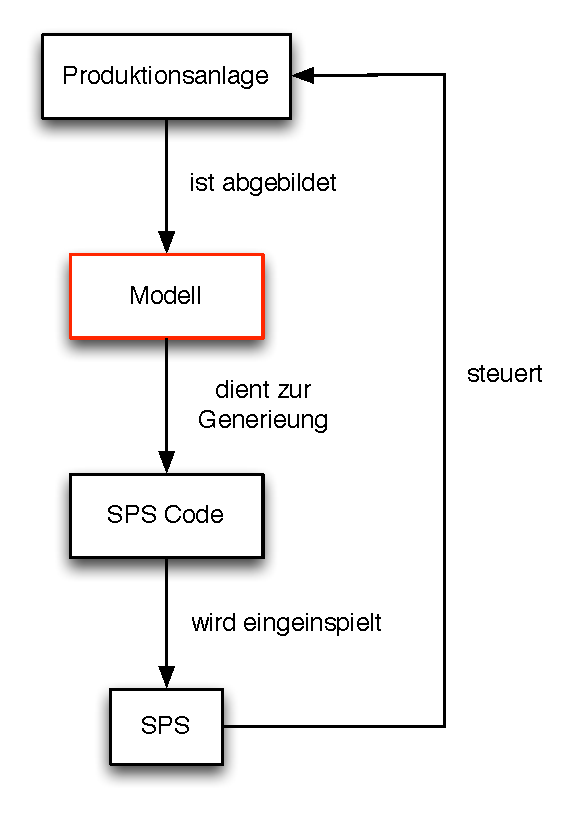
\includegraphics[width=0.37\textwidth]{graphics/konzept/konzept.pdf}
		\caption{Konzept für die modellbasierte Entwicklung der Steuerung}
		\label{fig:konzept}
\end{figure} \\
In der Abbildung~\ref{fig:konzept} ist zu sehen, dass die Produktionsanlage in einem Modell abgebildet ist. Aus diesem wird der \ac{SPS} Code generiert und im weiteren Schritt in die \ac{SPS} eingespielt. Daraufhin kann die Produktionsanlage gesteuert werden. 
%HSteuerungsaktivitäten und -funktionen, die es ermöglichen, endliche Mengen von Einsatzstoffen zu verarbeiten, indem diese unter Nutzung einer oder mehrerer Einrichtungen innerhalb eines endlichen Zeitraums einer geordneten

%Wir werden uns auf ist eine Norm für die chargenorientierte Fahrweise (Batch Control), die häufig als S88 oder SP88 bezeichnet wird. Sie ist eine Designphilosophie für Software, Ausrüstung und den Verfahrensablauf. 	

\section{Aufgabenstellung}
Im Rahmen des Projekts Batch\_it soll eine Visualisierung und Steuerung sowie eine modellbasierte Entwicklung der Steuerung für eine Laboranlage für Chargenprozesse, die sich durch eine chargenorientierte Fahrweise (Batch Control) kennzeichnet,  implementiert werden. Dies umfasst das Erstellen von Prozeduren nach dem \acs{IEC} 61512 Standard. Hierbei handelt es sich um Funktionen wie z.B. das Pumpen von Flüssigkeiten von Tank zu Reaktor oder das Heizen bzw. das Vermengen einer Flüssigkeit. Darüber hinaus werden daraus Rezepte nach dem \acs{IEC} 61512 Standard entwickelt. Zusätzlich werden Fehlerszenarien einer Produktionsanlage aufgestellt, die zur späteren Entwicklung einer Fehleranalyse dienen.Im weiteren Schritt wird eine Ontologie erstellt in der die Anlage abgebildet wird. Anhand dieser wird eine automatische Codegenerierung für die Steuerung der Anlage implementiert.
\section{Leitfaden durch die Arbeit}
In Kapitel 2 wird der aktuelle Stand der Verfahrens- und Anlagentechnik erarbeitet. Dabei wird die Hardware- und Softwarekomponente von Produktionsanlagen betrachtet und derzeitige Ansätze diskutiert. Im Rahmen dessen wird auf die konzeptionelle Planung einer Anlage und den Hardwareaufbau bzw. der Programmierung einer SPS eingegangen. Zusätzlich werden die Steuerungs- und Visualisierungsapplikationen für Produktionsanlagen ausarbeitet. Im letzten Teil des State Of The Art wird auf den aktuelle Stand der Technik in der modellbasierten Entwicklung der Steuerung eingegangen. Das Kapitel 3 gibt zunächst einen theoretischen Überblick des entwickelten Konzepts und erklärt ausführlich das Informationskonzepte sowie die Codegenerierung. Die Implementierung in Kapitel 4 zeigt die genauen Arbeitsschritte von der Planung der Anlage bis zur automatischen Entwicklung der Steuerung. 
Das Ergebnis wird in Kapitel 5 betrachtet bzw. interpretiert und im abschließenden Kapitel 6 wird eine Zusammenfassung und ein Ausblick in die Zukunft der Diplomarbeit gegeben. 
%Implementierung















%
% Chapter2

\chapter{State of the Art} \label{chapter:stateoftheart}

	% ##################################################################
	% Definition Prozessen, für die späterer Verwendung der Worte 
	% ##################################################################

	\section{Konzeptionelle Planung einer Anlage}
	Als essentiell geltendes Dokument der Vorplanung einer Anlage, ist das Rohr- \& Instrumentenfließschema eine Möglichkeit in der Anlagen- \& Verfahrenstechnik, ein vollständiges Abbild einer davon als Modell darzustellen. Die verwendeten Bauteile sind auf jedenfall namentlich beschrieben, können aber auch zusätzliche Informationen, die zum Verständnis der Verwendung beitragen, beinhalten.\\
	
	Ein Reaktor etwa, hat die hinreichende Bedindung eines Namens, sowie notwendige Parameter wie beispielsweise, welche Öffnungen als Ein- oder Ausgänge vorgesehen sind, ob sich ein Sensor oder Aktor darin befindet, oder ob er einen gewissen Nenndruck benötigt, um arbeiten zu können. Mit einfachen Verbindungslinien zwischen den Bauteilen, werden Rohre dargestellt. Diese können ebenso wiederum mittels Nenndruck, Rohrklasse oder gar einer Spezifikationsnummer beschrieben werden. Zusammenfassend werden somit im Allgemeinen in einem RI-Schema Apparate (z.B.: Tanks, Speicherbehälter, Reaktoren), Maschinen (z.B.: Pumpen, Verdichter) und Leitungen dargestellt.\\
	
	Die folgende Abbildung 2.1 \todo{Ist die Abbildungsnummer 2.1 noch aktuell?} stellt einen Aufbau einer simplen Anlage mit Hilfe des RI-Schemas dar.\\

	\begin{figure}[h!]
  		\centering
		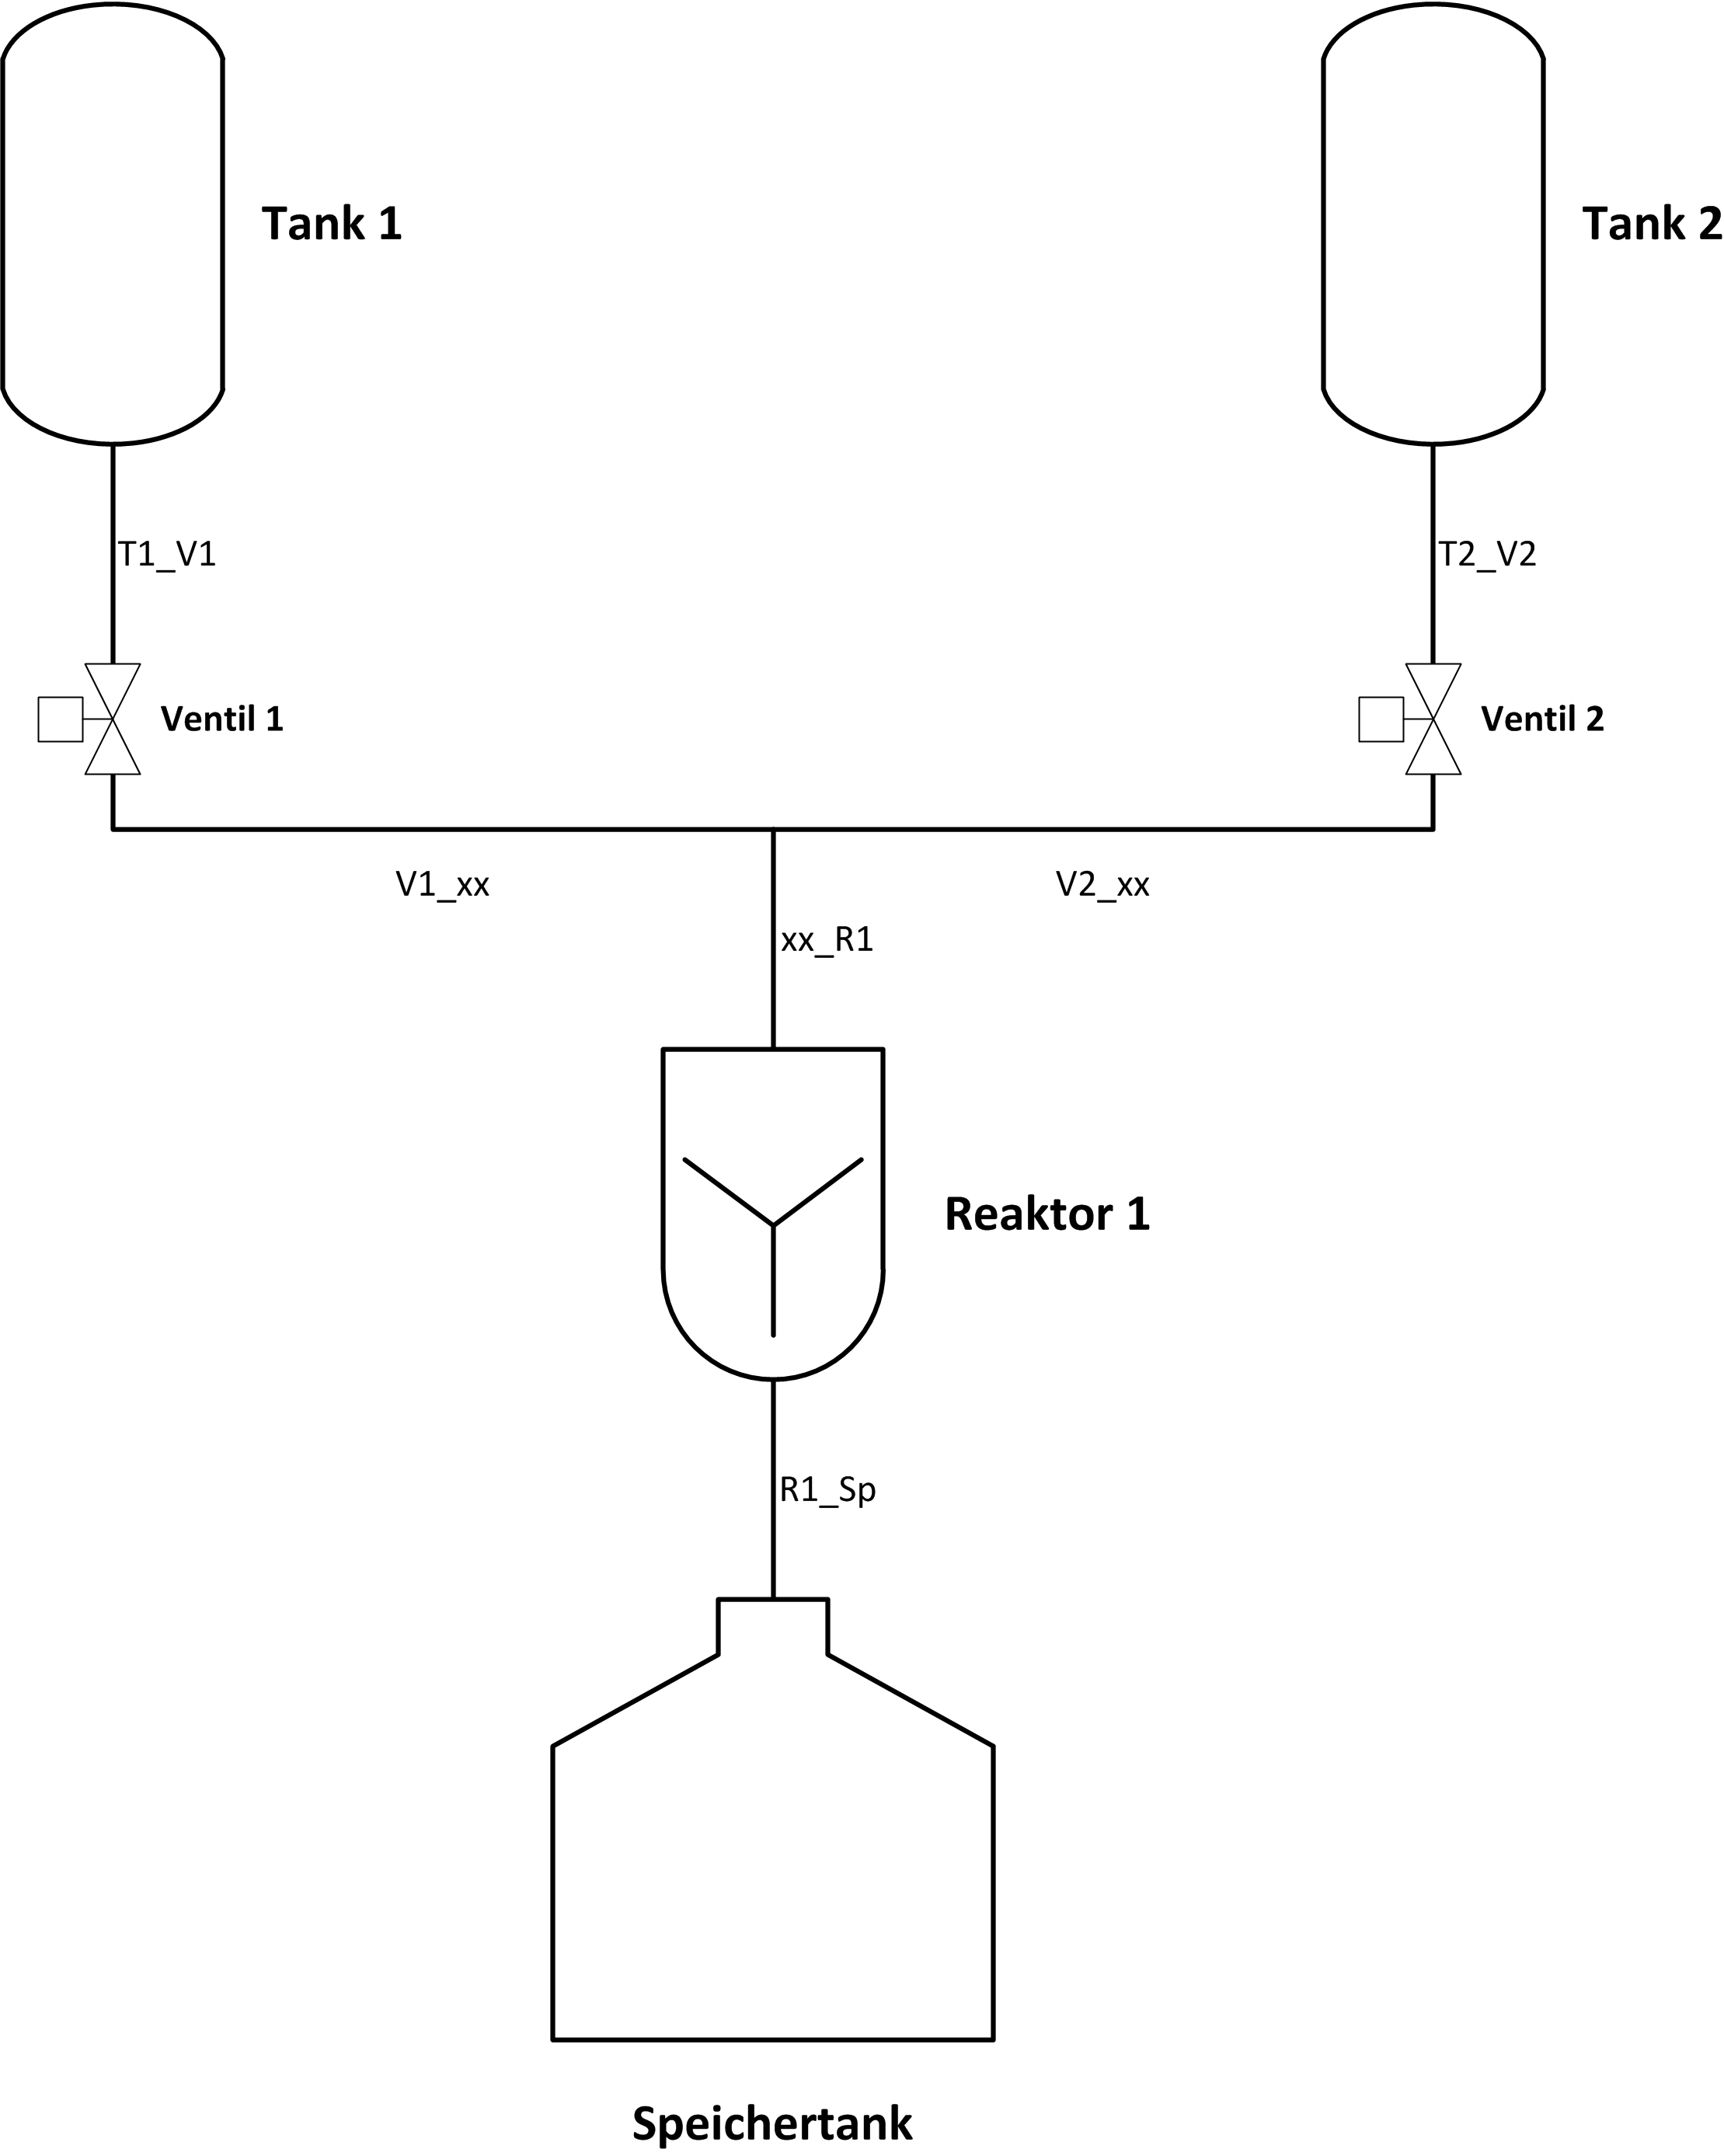
\includegraphics[height=0.7\textwidth]{graphics/stateoftheart/RI_SotA.jpg}
		\caption{Rohr- \& Instrumentenfließschema}
	\end{figure}

	\newpage
	\section{Definition eines Prozesses}
	Ein Prozess ist dadurch definiert, welche Arbeitsschritte bewerkstelligt werden müssen, um als Ergebnis das gewünschte Produkt zu erlangen. Die Anforderungen beziehungsweise das Zielprodukt formt somit den Arbeitsprozess.
	
	\begin{figure}[h!]
  		\centering
		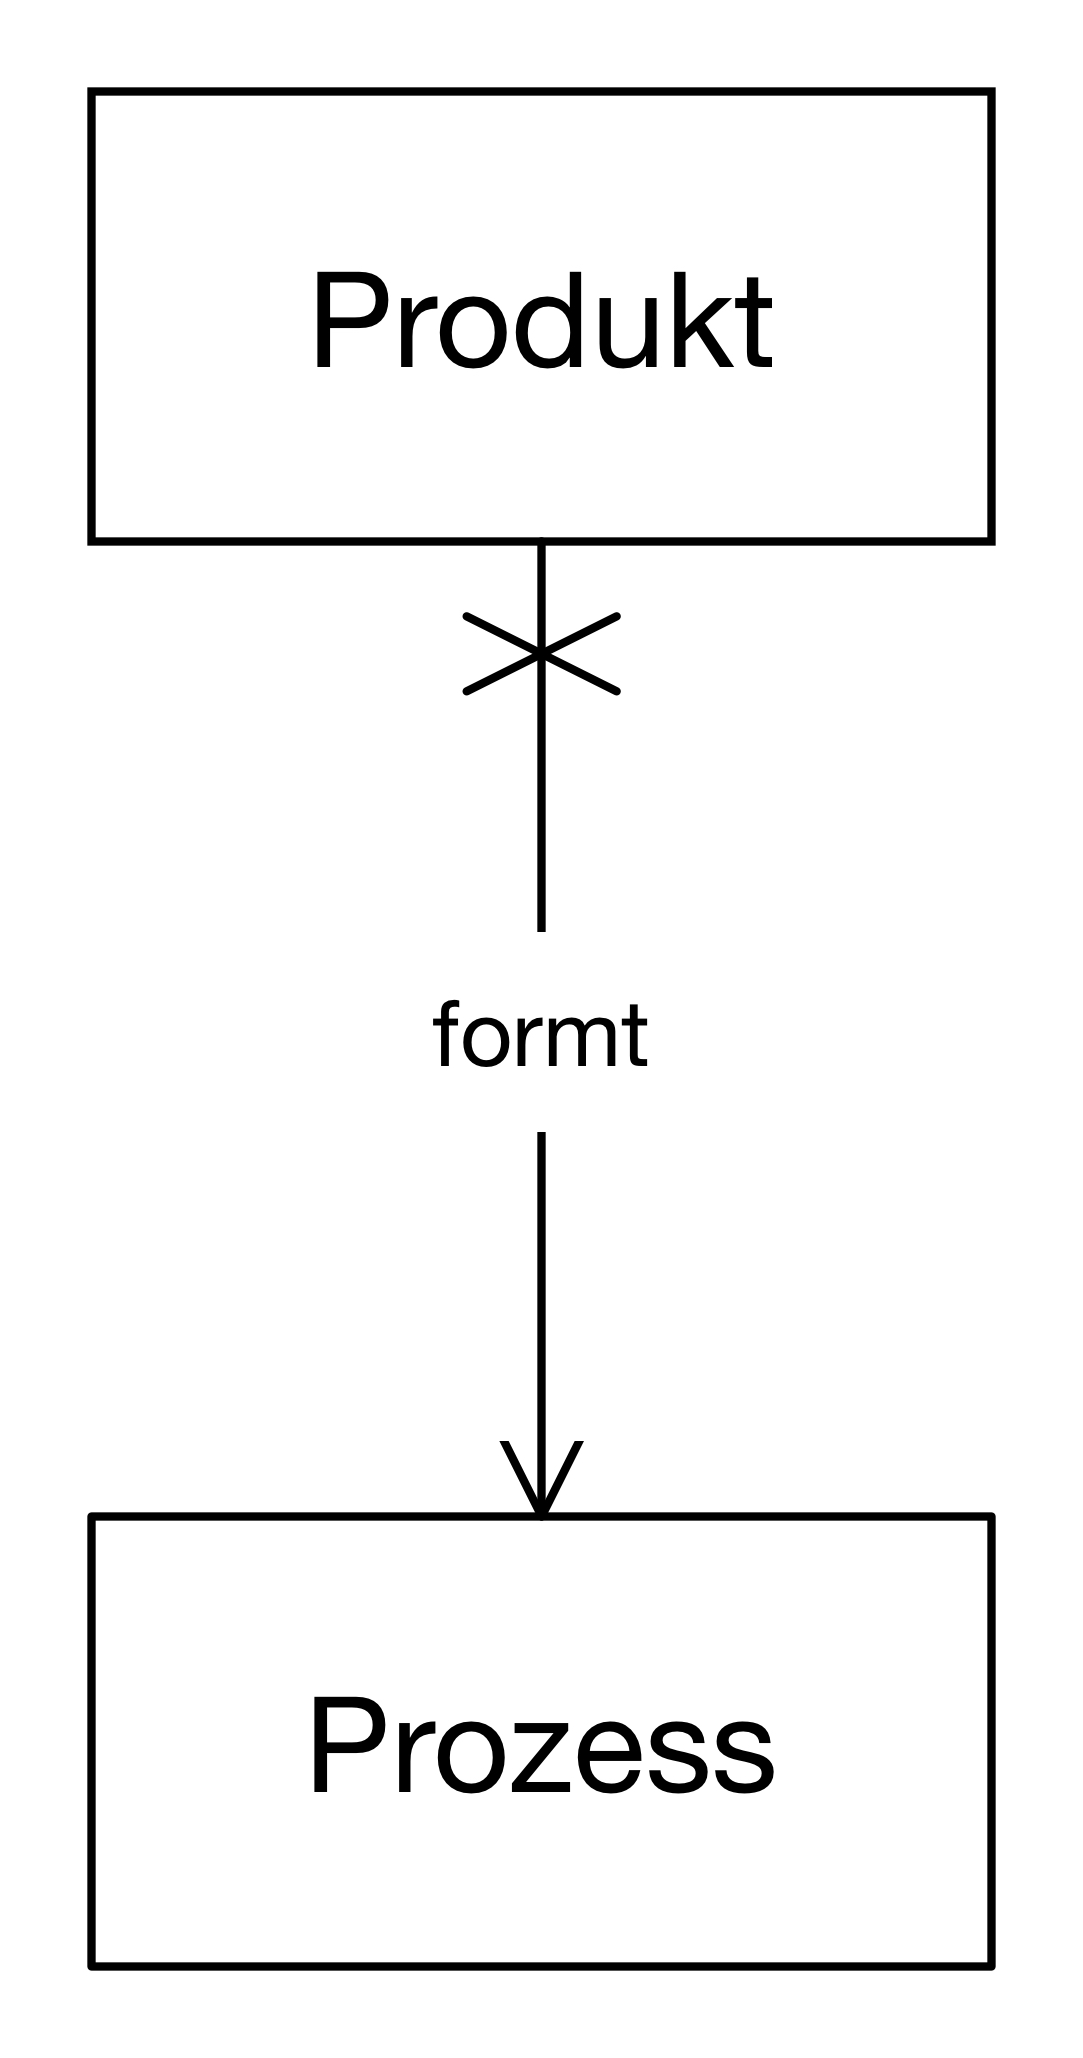
\includegraphics[height=0.5\textwidth]{graphics/stateoftheart/Prozess.jpg}
		\caption{Prozess}
	\end{figure}
	
	Laut der Norm DIN IEC 60050-351 ist ein Prozess wie folgt definiert:\\
		
	\textit{Ein Prozess repräsentiert einen Ablauf von sequentiell ausgeführten Aktivitäten innerhalb eines Systems zum Umwandeln, Lagern und Transportieren von Material, Energie oder Informationen.}\\

	Dabei ist wiederum tiefer ins Detail zu gehen, da es für technische Prozesse eine eigens entworfene, genauer spezifizierende Definition gibt.\\
	
	\textit{Ein technischer Prozess ist ein Prozess, dessen physikalische Werte gemessen, sowie mit technischen Mitteln beeinflusst werden.}\\
	
	Zu unterscheiden ist zwischen folgenden Prozessen:
	
	\begin{itemize}
		\item Diskreter Prozess
		\item Kontinuierlicher Prozess
		\item Chargenprozess
	\end{itemize}
	
	\subsection{Diskreter Prozess}
	Der diskrete Prozess wird häufig auch als \glqq Fertigungsprozess\grqq\space definiert, wobei es sich dabei im Grunde genommen um dasselbe handelt. Zu den Eigenschaften solch eines Prozesses gehört ein klar definierter Start- \& Endzeitpunkt. Der grundlegende Unterschied zu den noch folgenden ist jener, dass ausschließlich bei diskreten Prozessen die Formveränderung praktiziert wird, was wiederum bedeutet, dass es zu keiner stofflichen Strukturveränderung während des gesamten Ablaufs kommt. Zur Anwendung kommt diese Art in der Fertigung von mechanischen Produkten, wie etwa konkret in der Automobilindustrie.
	
	\subsection{Kontinuierliche Prozess}
	Konträr zum diskreten Prozess steht der häufig bei der Stromerzeugung zum Einsatz kommende kontinuierliche Prozess. Hierbei gibt es keinerlei festgeschriebenen Anfangs- \& Endzeitpunkt, was zur Folge hat, dass an jedem Ort immer die selben Zustände auftreten, wobei der Betrachtungszeitpunkt irrelevant ist. Bei diesen oft auch als stationär bezeichneten Prozessen wird etwa zu Beginn einer Produktionskette stets der selbe Zustand des Produkts auftreten. Dabei beschränkt sich die Verarbeitung auf formlose Stoffe, die da Sand, Flüssigkeiten oder Ähnliches sein können. Es kommt lediglich zu einer stofflichen Veränderung, wie einer chemischen Reaktion oder dem Aufheizen beziehungsweise Mischen mit einer anderen Substanz.
	
	\subsection{Chargenprozess}
	Bei der dritten und letzen Beschreibung handelt es sich um eine Art von Prozess, die teilweise Parallelen der diskreten und kontinuierlichen Prozesse aufweist. So wird abermals mit formlosen Materialien gearbeitet, welche ausschließlich stofflich verändert werden. Der ausschlaggebende Unterschied zu kontinuierlichen Prozessen ist jedoch, dass es klare Anfangs- \& Endzeitpunkte während des Prozesses gibt. So hat etwa das Füllen eines Tanks ein eindeutiges Endergebnis, über das nicht folgenlos hinausgegangen werden kann.\\

	Ableitbar aus den obigen Definitionen, müssen Anlagen auf Basis spezifischer Prozesse geplant und erbaut werden. Diese hat hingegen keinen Selbstzweck, sondern dient einzig und alleine nur dafür, einen oder mehrere Prozesse zu realisieren.\\

	% ##################################################################
	% Warum welche Hardware (Kriterien für unsere Nutzung, Umsetzbarkeit
	% ##################################################################
	\section{Hardwareaufbau einer SPS}
	
	Um die im späteren Verlauf aufbauende Hardware genauer beschreiben zu können, muss zu Beginn ein wenig thematisch ausgeholt werden. So hat der Begriff der Steuerung einen undenkbar hohen Stellenwert, welcher ebenso geklärt gehört.\\

	\todo{Ist die Abbildungsnummer 2.3 noch aktuell?}
	Unter einer Prozess - Steuerung versteht man nach der Norm DIN 19226, sowie in Abbildung 2.3 ersichtlich, einen Vorgang, bei dem durch Rückführen gemessener Prozesszustände, verglichen mit von der speicherprogrammierbaren Steuerung formulierten Parametern, Sollwerte zur Beeinflussung des gesamten Prozesses erzeugt werden. Im Gegensatz zu einer Regelung, muss der von einem Sensor ausgelesene Ist-Wert jedoch nicht zwanghaft rückgeführt werden.\\
	
	Der Steuerkreis besteht aus Sensoren, einem Steuerungsrechner, welcher meistens mittels einer SPS realisiert wird, sowie Aktoren. Die Steuerungseinheit selbst ist ein Rechner, mit dem Hauptaufgabenbereich, die programmierten, im Speicher abgelegten Anweisungen zyklisch auszuführen und über einfach anzusprechende Schnittstellen Daten einzulesen oder auszugeben. \cite{mseitz_sps} \\
	
	Der Begriff SPS wird in der Norm DIN EN 61131-1 (IEC 61131-1) wie folgt definiert:\\
	
	\glqq \textit{Ein digital arbeitendes elektronisches System für den Einsatz in industriellen Umgebungen mit einem programmierbaren Speicher zur internen Speicherung der anwenderorientierten Steuerungsanweisungen zur Implementierung spezifischer Funktionen wie z.B. Verknüpfungssteuerung, Ablaufsteuerung, Zeit-, Zähl- und arithmetische Funktionen, um durch digitale oder analoge Eingangs- und Ausgangssignale verschiedene Arten von Maschinen und Prozesse zu steuern. Die Speicherprogrammierbare Steuerung und die zugehörige Peripheriegerät (das SPS- System) sind so konzipiert, dass sie sich leicht in ein industrielles Steuerungssystem integrieren und in allen ihren beabsichtigten Funktionen einsetzen lassen.}\grqq \space \cite{sps_programmierung}\\
 
 	\begin{figure}[h!]
  		\centering
      	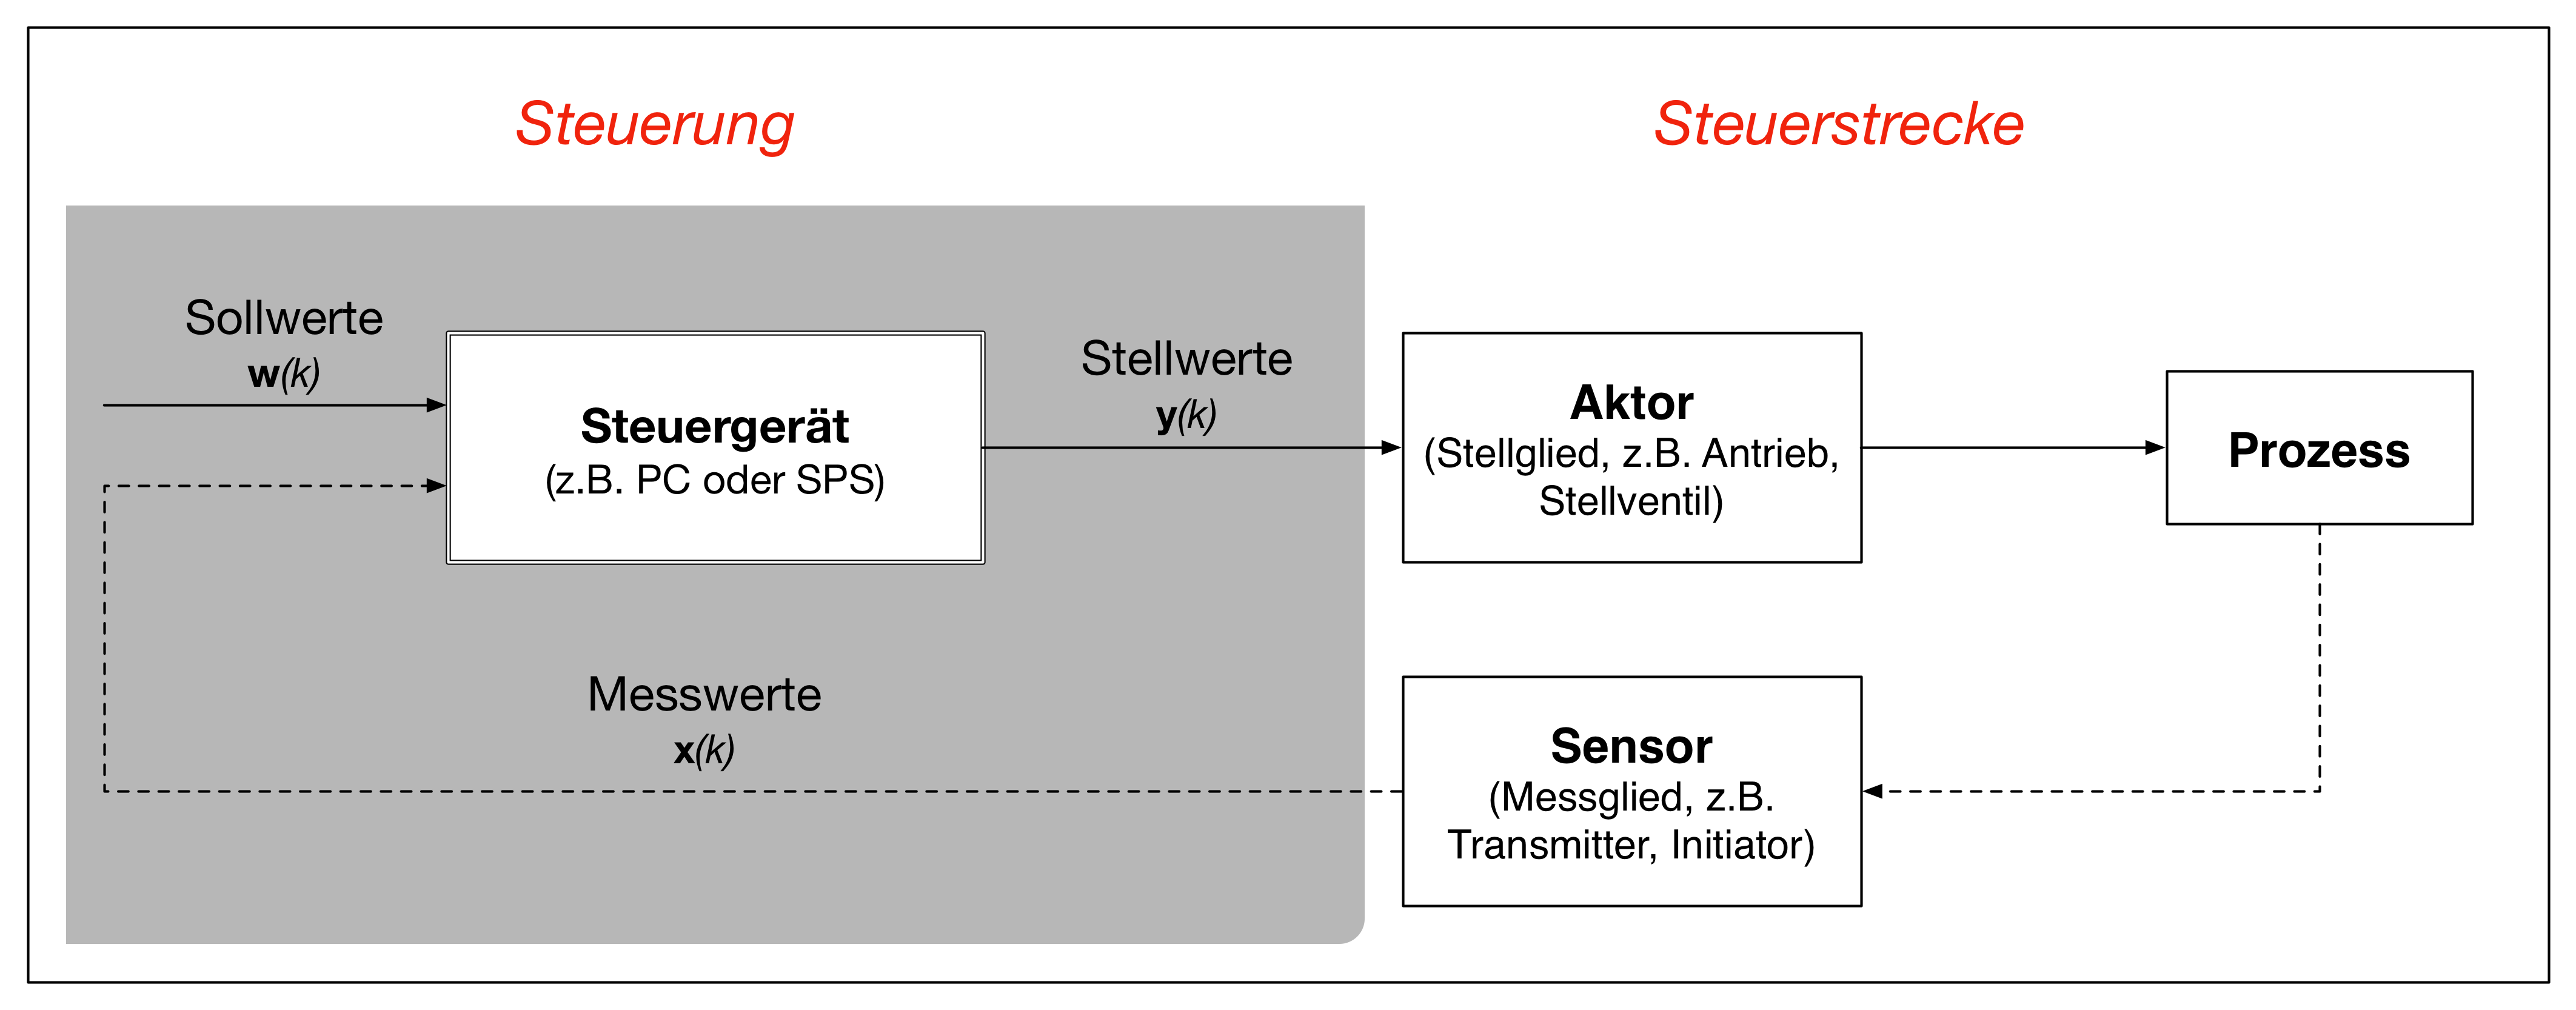
\includegraphics[width=1\textwidth]{graphics/stateoftheart/Aufbau_Steuerkreis_Selfmade.png}
  		\caption{Allgemeiner Aufbau eines Steuerkreises \cite{mseitz_sps}}
	\end{figure}	
 
 
 Im Detail gehört zum Aufbau einer SPS eine Stromversorgung, eine Verarbeitungseinheit (CPU), digitale, sowie analoge I/O Anschlüsse, eine Feldbusschnittstelle und das Programmiergerät, wobei es sich dabei heutzutage eigentlich ausschließlich um einen externen Computer handelt. Die Stromversorgung PS (\textbf{P}ower \textbf{S}upply) wandelt gleichzeitig die Netzspannung in eine 24-V-Gleichspannung um, mit der die Elektronik der SPS versorgt wird.\\
	
	Man unterscheidet mittlerweile drei verschiedene Aufbauarten bei SPSen
	
	\begin{enumerate}
  		\item Hardware - SPS
  		\item Slot - SPS
  		\item Soft - SPS
	\end{enumerate}

	\textbf{Hardware - SPS}\\\\
	Der im vorigen Abschnitt beschriebene Aufbau einer SPS bezieht sich auf die klassische Aufbauform einer \textit{Hardware - SPS}. Ihre Komponenten sind als gewöhnliche Einsteckkarten in einem Gehäuse oder Schaltschrank angeordnet und sind über einen Rückwandbus miteinander verbunden. Die Hardware - SPS benötigt einen externen PC als Programmiergerät.\\
	
	\textbf{Slot - SPS}\\\\
	Eine Slot - SPS ist eine Einsteckkarte für den PC, welche alle Module einer SPS enthält. Anstatt einer CPU befindet sich ein Co-Prozessor in ihr, auf dem ein eigenes multitaskingfähiges Betriebssystem läuft. Zusätzlich verfügt sie über einen sogenannten multi-ported RAM (ein geteilter Speicher, der sowohl für SPS, als auch für PC zugreifbar ist).\\
	
	\textbf{Soft - SPS}\\\\
	Zu guter Letzt gibt es die Soft - SPS, welche im Gegensatz zu den anderen Steuerungseinheiten eine reine Softwarelösung ist, die komplett auf der CPU des Host-PCs läuft und auch deren Hardware nutzt. Zur Ankopplung der Sensoren und Aktoren wäre eine Einsteckkarte zur Feldbuskopplung notwendig, die mit einem Prozessor zur Buskommunikation und einem dual-ported Ram ausgestattet ist.\\
	
	Die Vorteile der SPS im PC ergeben sich hauptsächlich dadurch, dass die rasante Entwicklung der PC-Leistungen für SPSen genau dafür genutzt werden kann.\\
	
	Die Informationsverarbeitung in einer SPS verläuft zyklisch. Die Verarbeitungsschritte lassen sich vereinfacht mit dem EVA - Prinzip beschreiben.
	
	\begin{itemize}
		\item \textbf{E}inlesen der Sensordaten
		\item \textbf{V}erarbeiten der Informationen im SPS-Programm
		\item \textbf{A}usgeben der Soll-Werte an die Aktoren
	\end{itemize}
	
	Die CPU fragt anfangs nacheinander alle Eingangskanäle ab und legt anschließend die Daten in den Arbeitsspeicher - es entsteht das sogenannte \glqq Eingangsabbild\grqq. Hierbei handelt es sich jedoch nicht um die aktuellen, sondern um die zum Abtastzeitpunkt ausgelesenen Werte. Die erstellten Programme werden ausschließlich von der CPU jeweils Schritt für Schritt abgearbeitet. Erst nach Abarbeitung \textbf{aller} Programme werden die im Ausgangsabbild abgelegten Sollwerte nacheinander an die Ausgangskanäle übertragen. \cite{mseitz_sps} \\ 
	
	Kleinere SPS - Hersteller versuchen ihre eigene spezifische Hardware möglichst kompatibel für fremde Software zu produzieren, um mit ihrem Produkt eine möglichst große Zielgruppe anzusprechen. Große Hersteller hingegen möchten ihr System eher geschlossen für den Zugriff mittels fremder Software halten, um die Kundenbindung auf den verschiedensten Ebenen der Automatisierungspyramide zu erhöhen.
	
	\begin{figure}[h!]
  		\centering
    	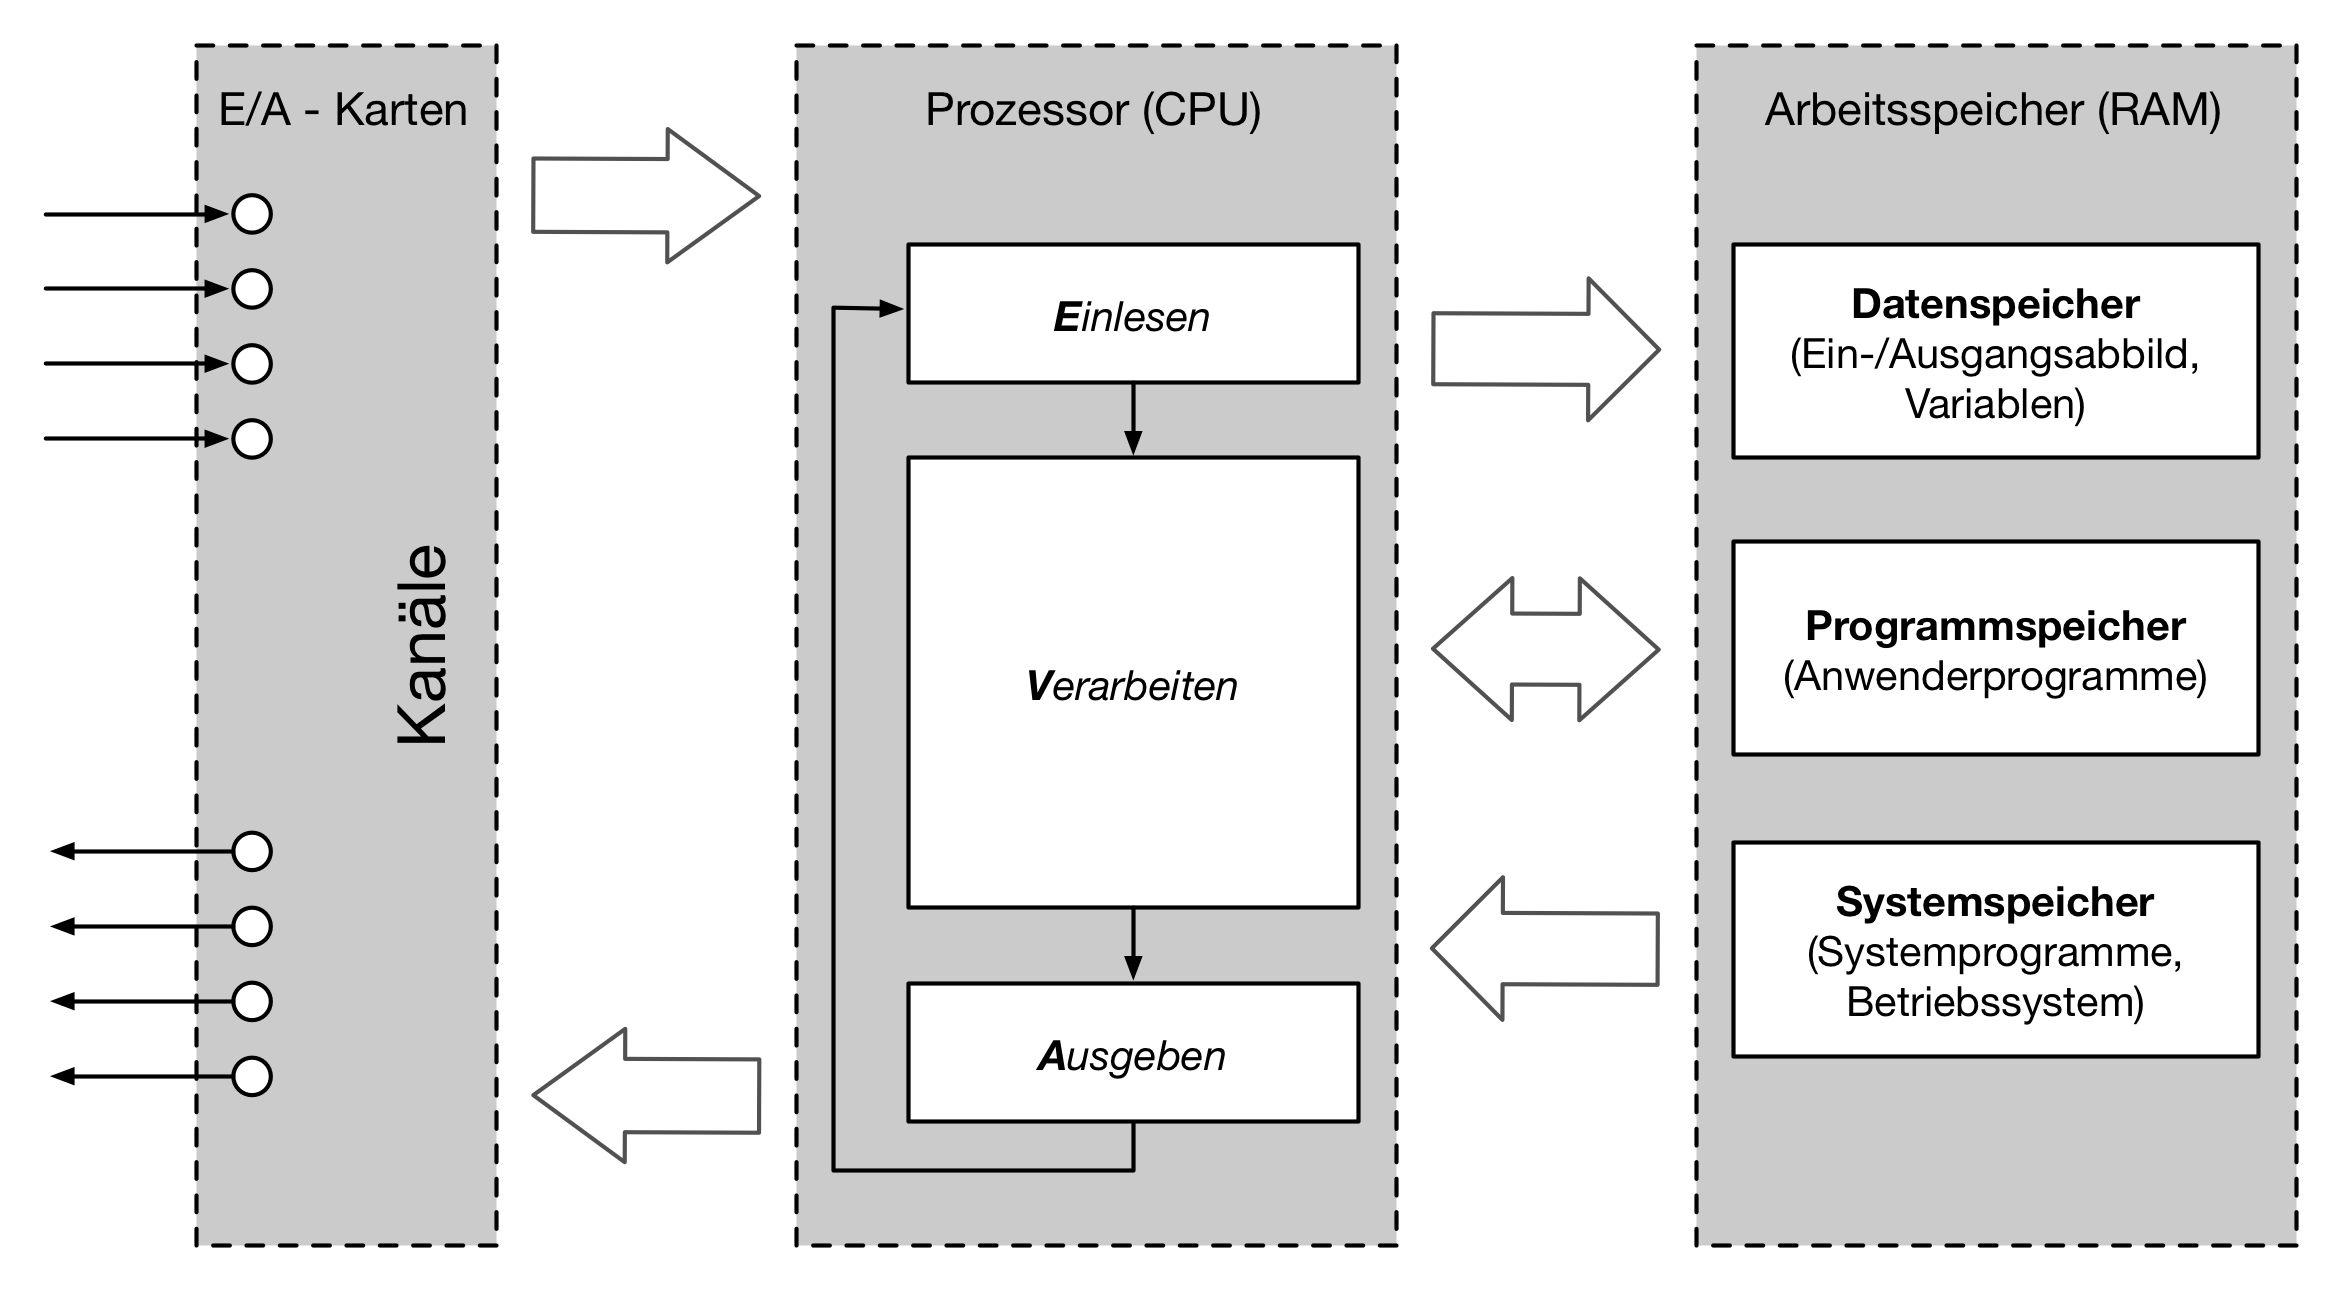
\includegraphics[width=1\textwidth]{graphics/stateoftheart/Signalverarbeitung_Selfmade.png}
  		\caption{Signalverarbeitung und Arbeitsweise einer SPS \cite{mseitz_sps}}
	\end{figure}
		
	% ##############################################################
	% Programmierung einer SPS - Wie funktioniert das grundsätzlich?
	% ##############################################################
	\section{Programmierung einer SPS}

	In der Automatisierungs- und Regelungstechnik gibt es zum Erfüllen der gegebenen Anforderung mehrere Wege um diese zu lösen. Genauer gesagt handelt es sich hierbei um ganze sechs verschiedene Programmiersprachen, um auf jede möglich auftretende, sowie spezifische Anforderung individuell eingehen zu können. Diese unterteilen sich wiederum in zwei differenzierbare Untergruppen. So gibt es zum einen die textbasierten Programmiersprachen
	
	\begin{itemize}
		\item[a)] Anweisungsliste (engl. \textit{Instruction List})
		\item[b)] Strukturierter Text (engl. \textit{Structured Text})
		\item[c)] Ablaufsprache (engl. \textit{Sequential Function Chart})
	\end{itemize}

	Im Gegensatz dazu gibt es noch die grafikbasierten Programmiersprachen
	
	\begin{itemize}
		\item[d)] Kontaktplan (engl. \textit{Ladder Diagram})
		\item[e)] Ablaufsprache (engl. \textit{Sequential Function Chart})
		\item[f)] Funktionsbausteinsprache (engl. \textit{Function Block Diagram})
	\end{itemize}
	
	Ziel dieser Vielfalt ist es, eine Vereinheitlichung der Programmierung von SPSen zu erreichen. Der Standard 61131 ist seit 1993 eingeführt und industriell etabliert. Mittlerweile schon in der dritten Edition verfügbar, und somit auch Objektorientierung unterstützend, sind die Programmiersprachen für zentrale \& eng gekoppelte Systeme ausgelegt.\\
	
	\textbf{a) Anweisungsliste}\\
	
	Diese textbasierte Programmiersprache nach der Norm IEC DIN EN 61131-3 ist sehr maschinennahe. Vergleicht man die Anweisungsliste aus Abbildung 2.5 \todo{Ist die Abbildungsnummer 2.5 noch aktuell?} mit höheren Programmiersprachen der Informatik, so ist es eine Art Assemblersprache, die normalerweise 1:1 den jeweiligen Maschinencode übersetzt. Es werden die einzelnen Anweisungen in der Reihenfolge geschrieben, wie sie die Maschine (CPU) abarbeiten soll (auch \glqq Stackorientierte Abarbeitung\grqq \space genannt). Ein großer Vorteil gegenüber allen graphischen Programmiersprachen ist die Tatsache, das AWL funktionell über diese hinausgeht, weil beispielsweise ein komplexer Zählvorgang mittels eines Kontaktplans nicht realisierbar sein könnte.	\cite{spslehrgang_struktur, egroetsch_sps}\\

	\begin{figure}[h!]
		\begin{framed}
			VAR\\
			s1: BOOL; \color{gray}//[input] Sensor Deklaration\\ \color{black}
			s2: BOOL; \color{gray}//[input] Sensor Deklaration\\ \color{black}
			s3: BOOL; \color{gray}//[input] Sensor Deklaration\\ \color{black}
			M: BOOL := 0; \color{gray}//[output] Motor Deklaration (muss initialisiert werden)\\ \color{black}
			END\_VAR\\\\
			LD s1; \color{gray}//[load] Lade den boolean-Wert ins Register\\ \color{black}
			OR s2; \color{gray}//Oder-Verknüpfung mit s1\\ \color{black}
			ANDN s3; \color{gray}//Und-Verknüpfung mit invertiertem Eingang\\ \color{black}
			ST \color{gray}//[store] Ergebnis wird in die Variable Motor geschrieben\\
		\end{framed}
		\caption{Beispiel einer Anweisungsliste}
	\end{figure}
	
	\color{black}
	\textbf{b) Strukturierter Text}\\
	
	Diese in Abbildung 2.6 \todo{Ist die Abbildungsnummer 2.6 noch aktuell?} angeführte Programmiersprache der Automatisierungstechnik orientiert sich an der Sprache Pascal, enthält aber neben dieser Sprache zugehörigen spezifischen Elementen aber auch noch SPS-typische Elemente. Geeignet ist ST am vorteilhaftesten für Aufgaben mit mathematischem Hintergrund, sowie zum Beschreiben komplexer Algorithmen. Auch für Rezept- und Datenverwaltung hebt sich diese Art der Programmierung durch enorme Vereinfachung vor. Typische Anweisungen für ST sind solche, die in höheren Sprachen durch Bedingungen oder Schleifen ausgeführt werden können \cite{grundlagen_automatisierungstechnik}
	\todo[inline]{Schauen ob die Figur \glqq Strukturierter Text\grqq \space an der richtigen Position ist.}
	
	\begin{figure}[h]
		\begin{framed}
		\color{black}
		VAR\\
		s1: BOOL; \color{gray}//[input] Sensor Deklaration\\ \color{black}
		s2: BOOL; \color{gray}//[input] Sensor Deklaration\\ \color{black}
		s3: BOOL; \color{gray}//[input] Sensor Deklaration\\ \color{black}
		M: BOOL := 0; \color{gray}//[output] Motor Deklaration ( muss initialisiert werden)\\ \color{black}
		END\_VAR\\
		M := (s1 OR s2) AND ( NOT (s3)); \color{gray}//ODER-Verknüpfung von s1 und s2, anschließendes UND-Verknüpfung von Ergebnis mit negiertem s3.\
		\end{framed}
		\caption{Beispiel eines strukturierten Textes}
	\end{figure}
	
	\color{black}
	\textbf{c, e) Ablaufsprache}\\
	
	Eine Sonderstellung unter den Sprachen zur Programmierung einer SPS nimmt die Ablaufsprache ein.
	\todo[inline]{Ablaufsprache noch genauer beschreiben!}
	\textbf{d) Kontaktplan}\\
	Die Darstellungsart des Kontaktplans ermöglicht SPS-Programmierern ein Programm auf graphischer Ebene zu erstellen und darzustellen. Ein KOP ist einem Stromlaufplan sehr ähnlich, um Programmieranfängern, die beispielsweise nur in der Elektronik tätig sind/waren und noch nie zuvor analytisch hinterfragten Code entwickelt haben, dein Einstieg zu erleichtern. Es werden Elemente wie Spulen, Öffner/Schließer, Eingänge/Ausgänge, usw... verwendet, die zu logischen Blöcken zusammengefasst werden können und so einen Teil des gesamten Programms ergeben. Ein Nachteil dieser standardisierten Programmiersprache ist jedoch, dass es nicht für alle möglichen Operationen auch ein einheitliches Symbol in einem Stromlaufplan gibt. Das wiederum bedeutet, dass bei komplexen Steuerungen oft eine Mischung aus KOP und der Funktionsbausteinsprache (FBS) verwendet wird.
	\todo[inline]{Schauen ob das Bild \glqq kop\_Selfmade\grqq \space an der richtigen Position ist.}
	\begin{figure}[h!]
  		\centering
    	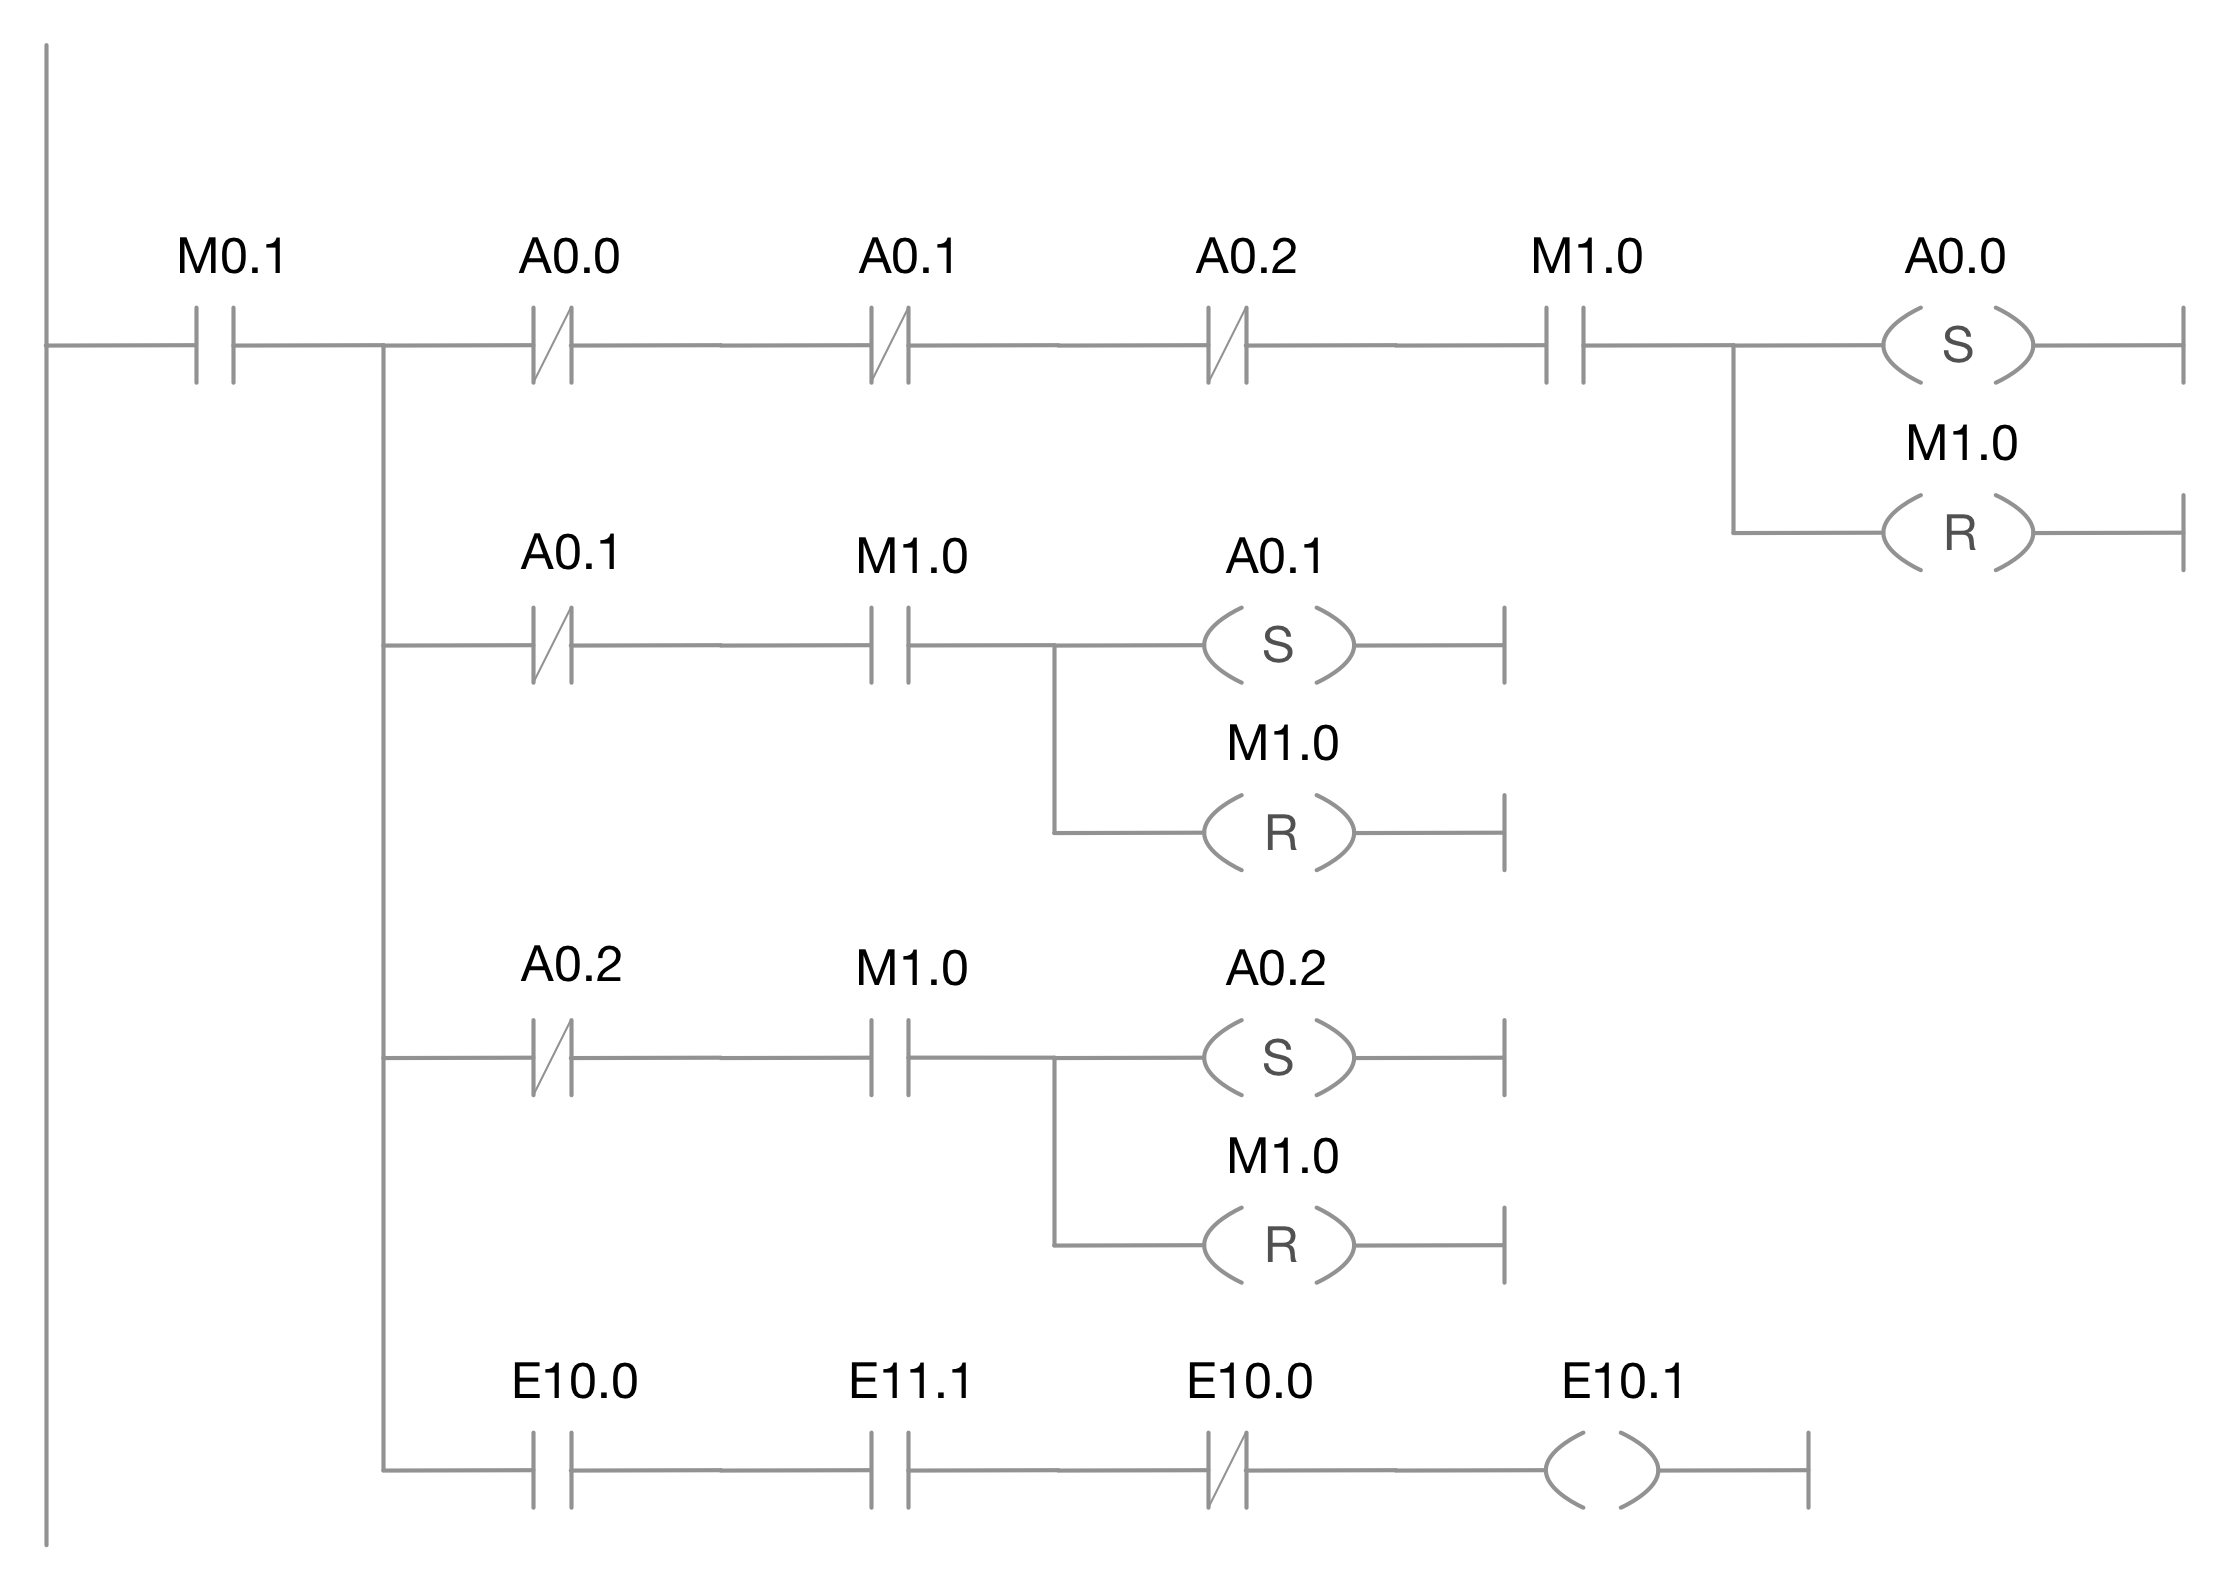
\includegraphics[width=0.8\textwidth]{graphics/stateoftheart/kop_Selfmade.png}
  		\caption{Beispiel eines Kontaktplans \cite{kontaktplan}}
	\end{figure}

	\newpage
	\textbf{f) Funktionsbausteinsprache}\\

	Diese graphische Programmiersprache verwendet für ihre Anweisungen logische Symbole der Boolschen Algebra. Diese Sprache ist insbesondere für Verknüpfungssteuerungen geeignet und deswegen bei Anfängern oder Programmier - Laien beliebt. Durch den einfachen graphischen Aufbau ist die Programmlogik relativ schnell zu erkennen und nachzuvollziehen.

	\begin{figure}[h!]
  		\centering
    	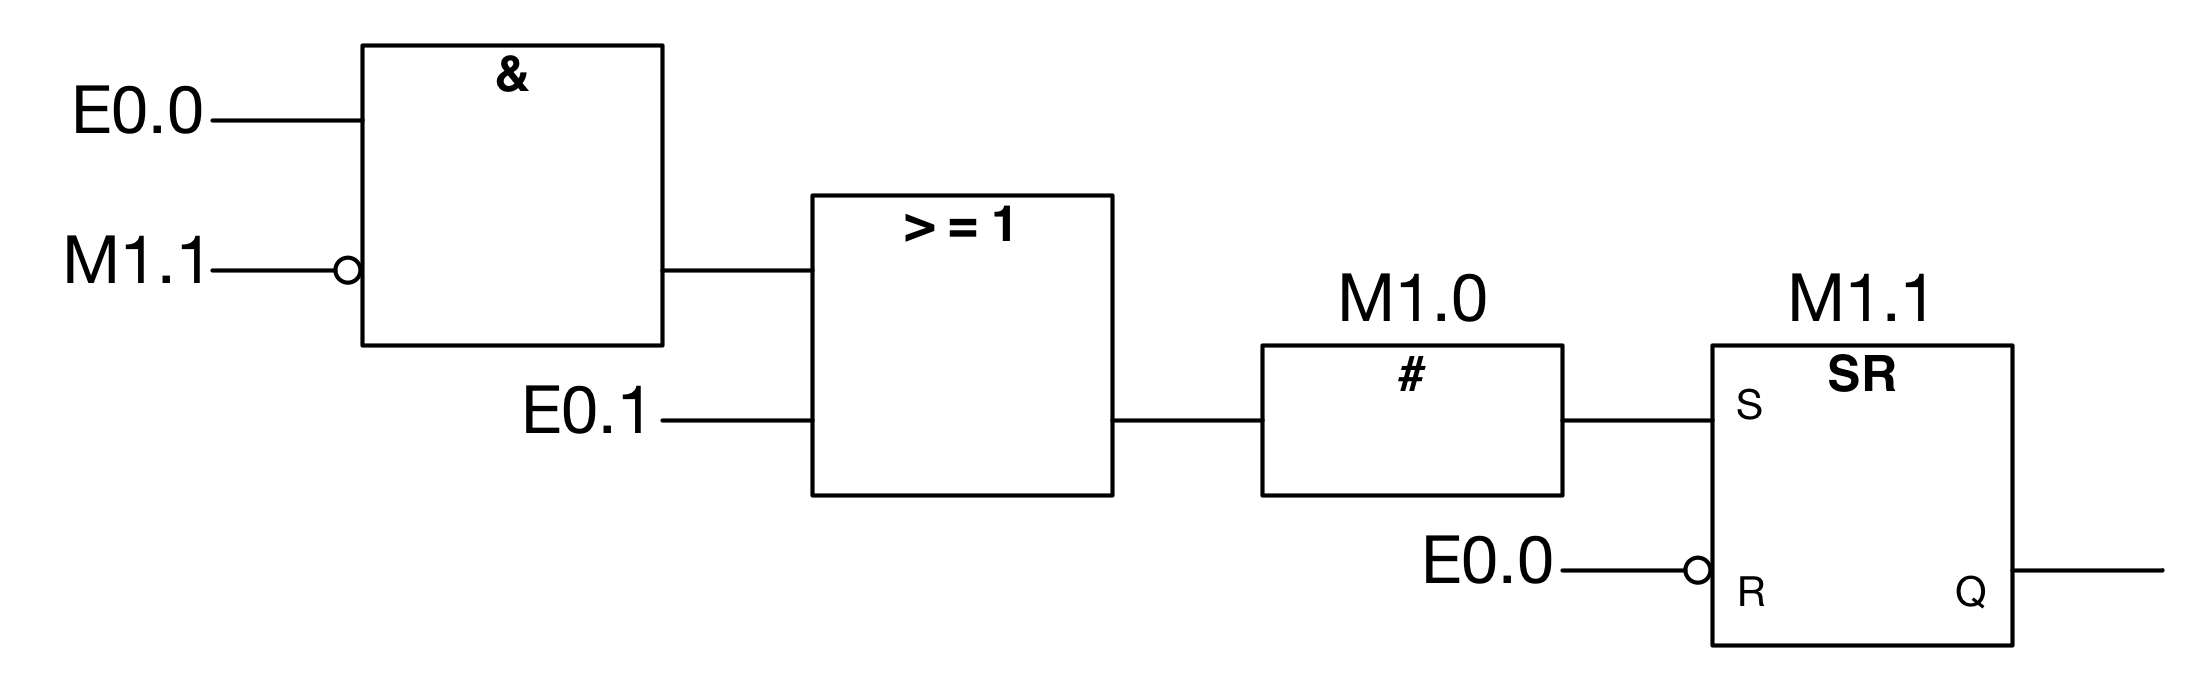
\includegraphics[width=0.8\textwidth]{graphics/stateoftheart/funktionsbausteinplan_Selfmade.png}
  		\caption{Beispiel eines Funktionsbausteinplans \cite{funktionsbausteinplan}}
	\end{figure}

\section{Prozeduren und Rezepte}
\subsection{Prozedur}
Die Prozedursteuerung bestimmt, daß einrichtungsorientierte Aktionen in einer geordneten Folge stattfinden, damit eine prozessorientierte Aufgabe ausgeführt wird. Prozedursteuerungen sind charakteristisch für chargenorientierte Prozesse. Sie sind die Art von Steuerung, die Einrichtungen in die Lage versetzt, einen Chargenprozess auszuführen.\\

%Quelle EN 61522
\begin{figure}[h!]
		\centering
		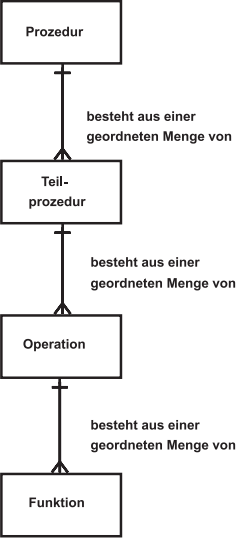
\includegraphics[width=0.4\textwidth]{graphics/stateoftheart/prozedursteuerung.png}
		\caption{Aufbau einer Prozedur}
\end{figure}
\newpage
\textbf{Prozedur}\\
Die Prozedur ist die höchste Stufe in der Hierarchie und legt die Strategie für die Ausführung einer umfassenden Verarbeitungsaktion, wie zum Beispiel der Herstellung einer Charge, fest. Sie wird durch eine geordnete Menge von Teilprozeduren bestimmt. Ein Beispiel für eine Prozedur ist „Produziere PVC“.\\

\textbf{Teilprozedur}\\
Eine Teilprozedur besteht aus einer geordneten Menge von Operationen, die bewirken, daß eine zusammenhängende Produktionssequenz in einer Teilanlage stattfindet. Es wird angenommen, daß zu jeder Zeit immer nur eine Operation in einer Teilanlage aktiv ist. Eine Operation wird in einer einzelnen Teilanlage vollständig ausgeführt. Gleichwohl können mehrere Teilprozeduren einer Prozedur konkurrierend ablaufen, jede in einer anderen Teilanlage.\\
Beispiele für Teilprozeduren sind:
\begin{itemize}
	\item Polymerisiere Vinylchlorid-Monomer.
	\item Gewinne Vinylchlorid-Rest zurück.
	\item Trockne PVC.
\end{itemize}
\textbf{Operation}\\
Eine Operation ist eine geordnete Menge von Funktionen, die eine größere Verarbeitungssequenz festlegt und die bewirkt, daß die verarbeiteten Stoffe von einem Zustand in einen anderen überführt werden, womit gewöhnlich eine chemische oder physikalische Umwandlung verbunden ist. Häufig ist es erwünscht, die Grenzen einer Operation auf Punkte in der Prozedur zu legen, wo die normale Verarbeitung sicher ausgesetzt werden kann.\\
Beispiele für Operationen sind:
\begin{itemize}
	\item Vorbereitung: Reaktor evakuieren und Reaktorwände mit Antifouling beschichten.
	\item Füllen: Destilliertes Wasser und Lösemittel hinzugeben.
	\item Reaktion: Vinylchlorid-Monomer und Katalysator zugeben, heizen und Absinken des Reaktordrucks abwarten.
\end{itemize}
\textbf{Funktion}\\
Das kleinste Element einer Prozedursteuerung, das eine prozessorientierte Aufgabe ausführen kann, ist eine Funktion. Eine Funktion kann in kleinere Teile unterteilt werden. Die Schritte und Übergänge, wie sie in der IEC 60848 beschrieben sind, dokumentieren eine Methode, um Unterteilungen einer Funktion zu definieren.\\
Ein Schritt kann eine oder mehrere Anweisungen ausgeben oder eine oder mehrere Maßnahmen bewirken, zum Beispiel:
\begin{itemize}
	\item Ein- und Ausschalten von Regelungen und zustandsorientierten Arten der Basisautomatisierung und Vorgeben ihrer Sollwerte und ihrer anfänglichen Ausgangswerte.
	\item Setzen, Löschen und Ändern von Alarmgrenzen und anderen Grenzwerten.
	\item Setzen und Ändern von Reglerkonstanten, Betriebsarten von Regelungen und Typen von Algorithmen.
	\item Lesen von Prozessvariablen, wie z. B. Gasdichte, Gastemperatur und Volumendurchfluß von einem Durchflußmesser, und Errechnen des Massendurchflusses durch den Durchflussmesser.
	\item Durchführen der Überprüfung der Bedienberechtigung.
\end{itemize}
Die Ausführung einer Funktion kann resultieren in:
\begin{itemize}
	\item Befehlen an die Basisautomatisierung.
	\item Befehlen an andere Funktionen (entweder in dem gleichen oder einem anderen Einrichtungsobjekt).
	\item der Erfassung von Daten.
\end{itemize}
Das Ziel einer Funktion ist es, eine prozessorientierte Aktion zu bewirken oder zu definieren, wogegen die Logik oder die Folge von Schritten, die die Funktion ausmachen, einrichtungsspezifisch ist.\\
Folgende Beispiele für Funktionen seien genannt:
\begin{itemize}
	\item Vinylchlorid-Monomer zugeben.
	\item Katalysator zugeben.
	\item Heizen.
\end{itemize}

\subsection{Rezept}
Rezepte sind Teil der Europäischen Norm EN 61512, welche den Aufbau bei der Chargenorientierten Fahrweise definiert.\\\\
„Ein Rezept ist eine Gesamtheit, die die Minimalmenge von Informationen enthält, die eindeutig die Herstellungsanforderungen für ein bestimmtes Produkt beschreibt. Rezepte bieten eine Methode, Produkte und die Art, wie diese Produkte hergestellt werden, zu beschreiben“.\\\\
In der Norm werden die vier Typen von Rezepten, die fünf Kategorien von Informationen, die ein Rezept enthält und wie sich diese Information bei den verschiedenen Rezepttypen verändert,  behandelt.\\\\
Es können Unternehmensintern noch eigene Rezepttypen verwendet werden, falls die definierten nicht alle benötigten Anforderungen abdeckt, ausserdem kann es sein, dass für ein Produkt mehrere Rezepte bestehen, wenn dieses zum Beispiel in verschiedenen Werken produziert wird und dadurch unterschiedliche Abläufe beinhaltet.\\

\subsubsection{Rezepttypen}
%Quelle EN 61522
\begin{figure}[h!]
		\centering
		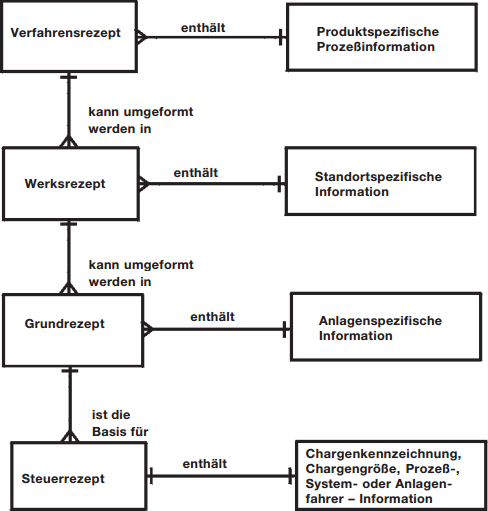
\includegraphics[width=0.6\textwidth]{graphics/stateoftheart/rezepttypen.png}
		\caption{Zusammenhang der Rezepttypen}
\end{figure}
„Verfahrens- und Werksrezept beschreiben die Vorgehensweise, also wie im Prinzip produziert wird. Grund- und Steuerrezept beschreiben die Aufgabe, also wie mit den tatsächlichen Betriebsmitteln zu produzieren ist.“
\\\\
\textbf{Verfahrensrezept}\\
Das Verfahrensrezept ist ein Rezept auf Unternehmensebene, das als Grundlage für Rezepte auf niedrigeren Ebenen dient. Das Verfahrensrezept wird ohne spezifische Kenntnis der Anlagenausrüstung erstellt, die zur Herstellung des Produktes benutzt werden wird. Es bestimmt die Rohstoffe, ihre relativen Mengen und die erforderliche Verarbeitung, allerdings ohne Bezug zu einem bestimmten Werk oder der in diesem Werk verfügbaren Ausrüstung. Es wird von Personen mit Kenntnissen der Chemie und den Verarbeitungsanforderungen erstellt, die für das betreffende Produkt typisch sind, und gibt deren Interessen und Überlegungen wieder.\\\\
Das Verfahrensrezept kann für die unternehmensweite Planung und für Investitionsentscheidungen benutzt werden. Es kann ein Teil von Produktionsvorgaben sein oder von solchen in Bezug genommen werden und kann als solches für die Produktionsplanung und zur Information von Kunden und Behörden verwendet werden.
\\\\
\textbf{Werksrezept}\\
Das Werksrezept ist spezifisch für ein bestimmtes Werk. Es ist eine Kombination von werksspezifischer Information und dem Verfahrensrezept. Es wird gewöhnlich aus einem Verfahrensrezept abgeleitet, um die Bedingungen einer bestimmten Produktionsstätte zu erfüllen, und bietet einen für werksbezogene, langfristige Produktionsplanung erforderlichen Detaillierungsgrad.
\\\\
\textbf{Grundrezept}\\
Das Grundrezept ist die Rezeptstufe, die auf eine Anlage oder eine Gruppe von Einrichtungen einer Anlage ausgerichtet ist. Ein Grundrezept kann vom Verfahrensrezept oder vom Werksrezept abgeleitet werden. Es kann mehrere von einem Werksrezept abgeleitete Grundrezepte geben, von denen jedes den Teil des Werksrezeptes abdeckt, der in einer Anlage ausgeführt werden kann. Das Grundrezept kann produktspezifische Informationen enthalten, wie sie zur detaillierten Produktionsplanung erforderlich sind, wie zum Beispiel Informationen über Prozesseinsätze oder Anforderungen an die Einrichtung.\\\\
Das Grundrezept ist eine unverzichtbare Rezeptstufe, da ohne es keine Steuerrezepte erzeugt und daher keine Chargen produziert werden können.
\\\\
\textbf{Steuerrezept}\\
Das Steuerrezept entsteht als eine Kopie einer bestimmten Version des Grundrezeptes und wird anschliessend wie erforderlich durch Informationen für Dispositionsplanung und Ausführung verändert, um spezifisch für eine einzelne Charge zu sein. Es enthält produktspezifische Prozessinformationen, wie sie zur Produktion einer bestimmten Charge erforderlich sind. Es bietet den Detaillierungsgrad, wie er zum Start und zur Überwachung der Einrichtungsprozedurobjekte einer Anlage erforderlich ist. Es kann verändert worden sein, um die tatsächlichen RohstoffQualitäten und die tatsächlich eingesetzte Ausrüstung zu berücksichtigen. Die Auswahl von Teilanlagen und entsprechende Skalierung kann jederzeit durchgeführt werden, bevor diese Information benötigt wird.
\subsubsection{Bestandteile des Rezeptes}

\textbf{Rezeptkopf}\\
Die organisatorische Information im Rezept wird als Rezeptkopf bezeichnet. Typische Informationen im Rezeptkopf kann die Rezept- und Produktidentifikation, die Versionsnummer, den Rezeptersteller, das Ausgabedatum, Freigaben, Status und andere organisatorische Angaben enthalten.
\\\\
\textbf{Stoff- und Produktionsdaten}\\
Die Stoff- und Produktionsdaten sind eine Kategorie von Rezeptinformation, die Prozesseinsätze, Prozessparameter und Prozessausstöße umfasst.
Ein Prozesseinsatz besteht aus Bezeichnung und Menge eines Rohstoffs oder eines anderen Betriebsmittels, das zur Herstellung des Produktes erforderlich ist.
Ein Prozessparameter enthält detaillierte Information wie zum Beispiel Temperatur, Druck und Zeit, die wesentlich für das jeweilige Produkt ist.  Prozessparameter können als Sollwerte, Vergleichswerte oder in logischen Bedingungen verwendet werden.
Ein Prozessausstoß besteht aus Bezeichnung und Menge eines Stoffs, die als Ergebnis einer Ausführung des Rezeptes erwartet wird.
\\\\
\textbf{Anforderungen an die Einrichtung}\\
Anforderungen an die Einrichtung schränken die Auswahl der Einrichtungen ein, die schließlich eingesetzt werden, um einen bestimmten Teil der Prozedur durchzuführen. Im Verfahrens- und im Werksrezept werden die Anforderungen an die Einrichtung typischerweise in allgemeiner Weise, wie zum Beispiel zulässigen Werkstoffen und erforderlichen Verarbeitungscharakteristika angegeben.
\\\\
\textbf{Rezeptprozedur}\\
Die Rezeptprozedur beschreibt die Strategie, um einen Prozess durchzuführen. Verfahrensrezeptprozeduren und Werksrezeptprozeduren sind unter Benutzung der im Prozessmodell beschriebenen Ebenen strukturiert, da diese Ebenen es gestatten, den Prozess in einrichtungsunabhängiger Art zu beschreiben. Grundrezeptprozeduren und Steuerrezeptprozeduren werden unter Benutzung der Prozedurelemente des Prozedurmodells beschrieben, da diese Prozedurelemente einrichtungsbezogen sind.

\subsubsection{Einrichtungssteuerung}
Das Steuerrezept selbst enthält nicht genügend Information, um die Anlage zu betreiben. Daher wird es mit der Einrichtungssteuerung, die tatsächlich die Einrichtungen zum Betrieb und zur Produktion von Chargen veranlasst, verknüpft. Die Einrichtungssteuerung wird nicht als Teil des Rezeptes angesehen.
%Quelle EN 61522
\begin{figure}[h!]
		\centering
		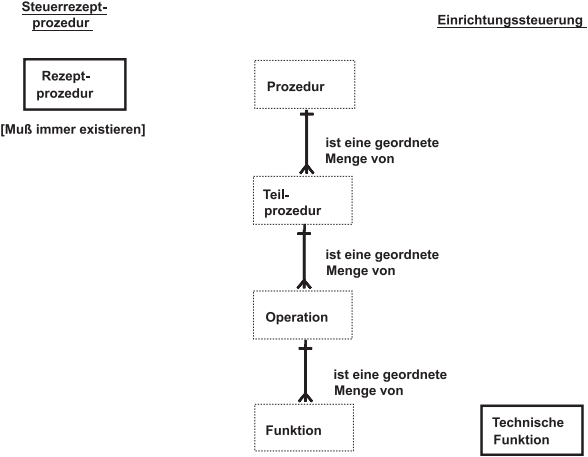
\includegraphics[width=0.8\textwidth]{graphics/stateoftheart/steuerrezeptprozedur_einrichtungssteuerung.png}
		\caption{Abgrenzung von Steuerrezeptprozedur und Einrichtungssteuerung}
\end{figure}
\\

\section{Visualisierung von Produktionsanlagen}
\subsection{SCADA}
(Supervisory Control And Data Acquisition)\\
Ein SCADA System ist im Allgemeinen eine Sammelstelle für alle aus der Anlagen generierten Werte. Diese Daten müssen dann weiterverarbeitet werden um aus ihnen Analysen zu erstellen.\\
Zu den Elemente eines SCADA Systems gehören:\\
\\
%todo Quelle Scada
%http://www.engineersgarage.com/articles/scada-systems?page=1
%10 März 2015
\textbf{SCADA Master Station Computer Systems}\\
Sammelstelle für Echtzeitdaten die von RTUs generiert werden. Meist herkömmliche Computer Hardware.\\
\\
\textbf{Human-Machine Interface}\\
Aus den gesammelten Daten Analysen (Prognosen, Diagnosen) so aufbereiten das sie für den Menschen leicht verständlich dargestellt werden.\\
\\
\textbf{Remote Terminal Units (RTUs)}\\
Sensoren die Physikalische Änderungen in der Anlage mit einem Signalumformer in Elektrische Werte umwandelt. Je nachdem was gemessen werden soll, entstehen Analoge (Füllstand, Helligkeit, Druck, ...) oder Digitale (z.B. Status eines Geräts) Werte.

\subsection{HMI}
Die Visualisierung einer Produktionsanlage ist ein wesentlicher Punkt der Datenverarbeitung und wird oft als Benachrichtigungszentrale benutzt. Meist werden in diesen in Echzeit aktualisierte Statuswerte sowie Benachrichtigungen zu unerwarteten Ereignissen angezeigt. Die hierfür benötigten Daten müssen von der SPS in die Visualisierungssoftware übermittelt werden. Da dies ein sehr aufwendiger Prozess ist, gibt es SCADA-Systeme die all diese Funktionen vereinen.\\
\\
Für dieses Projekt wurde eine Umsetzung in der SCADA Software zenon verlangt, daher wird im weiteren nur noch über die Visualisierung in zenon's HMI System (zenon Supervisor) gesprochen.\\
\\

%Quelle http://www.protec.at/dienstleistungen/visualisierung
%Quelle http://www.protec.at/tl_files/protec/uploads/Bilder_Logos/Visualisierung/visualisierung2.jpg
\begin{figure}[hbt!]
 \centering
  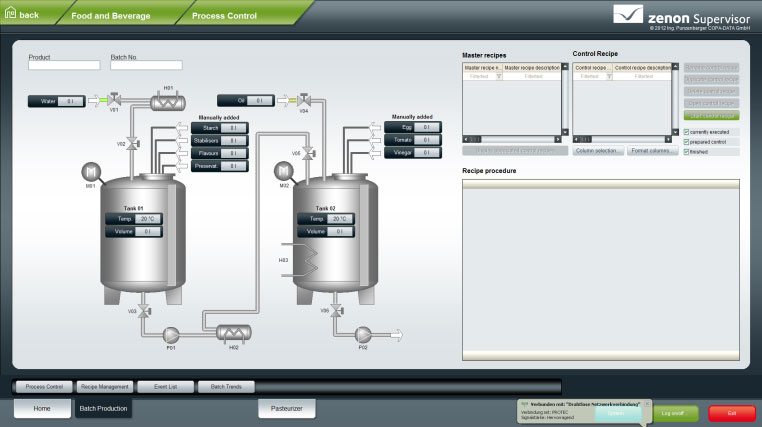
\includegraphics[width=1\textwidth]{graphics/stateoftheart/zenon_visualisierung}
  \caption{Beispiel Visualisierung in Zenon Supervisor}
\end{figure}


\newpage

\section{Modellbasierte Entwicklung der Steuerung}
Das Gebiet der Modellbasierten Entwicklung bzw. der automatisierten Codegenerierung aus einem Modell als ganzes kann man nicht wirklich als State of the Art erklären.\\

Wenn man sich jedoch die Gebiete als einzelnes anschaut, erkennt man das diese im heutigem Betrieb eingesetzt werden.
\subsection{Modell}
Ein Modell der gesamten Anlage wird schon im frühen Stadium der Entwicklung in Form eines RI-Fließschemas hergestellt um klar zu definieren welche Bauteile benötigt werden und welches mit welchem Bauteil verbunden ist. Dies ist nur das erste Modell das in der Industrie eingesetzt wird.\\
\\
Oft werden aber mehr Informationen benötigt als im RI-Fließschema ersichtlich sind, weswegen man auf eine andere Methode umsteigen muss ein Modell abzubilden.\\
Auf die gängigsten Methoden (XML, Ontologie, UML) wird in den nächsten Punkten genauer eingegangen.
\subsection{XML}
XML ist ein Textbasiertes Dateiformat das, obwohl es für Dokumente gedacht ist, oft für das Abbilden von Daten Strukturen verwendet wird.
\\
Ähnlich wie in HTML verwendet auch XML Tags, der unterschied besteht darin das XML keine vorgefertigten Tags besitzt und der Benutzer diese erstellt. Genau diese Benutzerdefinierten Tags ergeben die XML Struktur welche, was essentiell ist, von alleine nur ein Textfile ist und keine Funktionen besitzt.
\\
\lstinputlisting[language=XML,belowcaptionskip=5pt,caption=XML Sample Code]{extra/sample.xml}
Der Aufbau einer XML Datei ist leicht zu erklären: Es gibt 1 rootElement das den Anfang und das Ende des Inhaltes markiert, zwischen dem Start- und Endtag befinden sich weitere Tags die das Dokument oder die Struktur genauer beschreiben. Jeder Tag kann Attribute besitzen die es weiter definieren. Zwischen einem Start- und Endtag können sich entweder weitere Tags oder einfacher Text befinden.
\\
Einsatz findet XML meist in Programmen oder Webseiten die größere Mengen an Daten bzw. Befehle Systemunabhängig übertragen sollen. Grund dafür ist unter anderem die Tatsache dass Mensch und Maschine die Datei ohne Übersetzung/Kompilieren lesen und verstehen kann.\\
Doch auch wenn ein Mensch XML-Dateien lesen kann, dauert es länger die Struktur eines Textes, im vergleich zu einer Grafischen Darstellung, zu verstehen.\\ 
Dafür gibt es andere Werkzeuge, die auf XML basieren aber eine Grafische Darstellung erzeugen.
\subsection{Ontologie}
%todo Quelle Ontologie
%http://plato.stanford.edu/entries/logic-ontology/
\begin{displayquote}... we have at least two parts to the overall philosophical project of ontology: first, say what there is, what exists, what the stuff is reality is made out off, secondly, say what the most general features and relations of these things are.
\end{displayquote}
Eine Ontologie ist ein auf XML basierendes Konstrukt das einem das Abbilden von Dingen und deren Relationen ermöglicht. Um solch Komplexe Zustände darzustellen stehen einem neben einfachen Entitäten(Dinge) auch Eigenschaften zur verfügen.\\
\\
\textbf{Allgemeiner Aufbau einer Ontologie}\\
Das Modell an sich ohne zusätzliche Attribute oder Eigenschaften ist vom Aufbau her so zu erklären: Es gibt ein 'Thing' von dem alles aus geht (das root Element bei XML). Von diesem Punkt aus können weitere Entitäten abgeleitet werden (Eine Vererbung, vergleichbar mit einem Stammbaum). Die neu erstellte Entität ist immer noch ein Thing, jedoch genauer definiert. Es gibt keine Grenzen oder Vorschriften in welche Tiefe diese Definition gehen muss und kann daher für sehr Komplexe aber auch Simple Modelle eingesetzt werden.\\

\begin{figure}[hbt!]
 \centering
  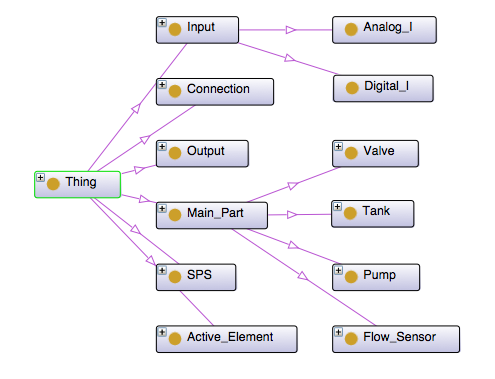
\includegraphics[width=1\textwidth]{graphics/stateoftheart/Ontology_Aufbau}
  \caption{Aufbau einer Ontologie}
\end{figure}

Wie in Abbildung 1 zu erkennen erhält man so die Struktur des Modells, jedoch werden oft weitere Informationen zu den einzelnen Objekten/Entitäten benötigt welche als Eigenschaften abgespeichert werden.\\
Dies ermöglicht ein Modell aufzubauen das nicht nur die Struktur abbilden kann, sondern komplexe Netzwerke zu konstruieren.\\
\\
\noindent \textbf{Objekt Eigenschaften}\\
Objekt Eigenschaften werden benötigt um Relationen zwischen den einzelnen Objekten genauer zu beschreiben.\\ 
Wie kann man einen Tank mit einer Pumpe verbinden? Genau dafür gibt es Objekt Eigenschaften. Für diesen zweck kann man eine Eigenschaft mit dem Namen 'verbunden\_mit' erstellen, und diese dann dem Tank beifügen. So ergibt sich die Relation: Tank verbunden\_mit Pumpe.\\
\\
\textbf{Daten Eigenschaften}\\
Daten Eigenschaften werden benötigt um Objekte genauer zu beschreiben. 
\\
Beispiel für ein Modell einer Produktionsanlage ist es etwaigen Sensoren im Modell einen Wertebereich festzulegen in welchem dieser arbeitet bzw. was für Werte dieser sammelt/zurückgibt: Ein Füllstandsensor mit einem Wertebereich von 4-20V, wobei 4V=Leer und 20V=Voll bedeutet, kann in einer Ontologie mit wenigen Data Properties abgebildet werden.

\subsection{UML}
UML ist, wie eine Ontologie, eine auf XML basierte Modellierungssprache.
%TODO Quelle UML
%Quelle OMG Unified Modeling LanguageTM (OMG UML), Infrastructure
Das Ziel von UML ist es, System Architekten, Software Ingenieuren und Software Entwicklern ein Werkzeug zur Analyse, Design, Implementation von Softwarebasierenden Systemen, sowie für Modell Entwicklung und ähnliche Prozesse zu bieten.\\
\\
Mit Hilfe von UML können viele verschiedene Arten von Diagrammen erstellt werden, für dieses Projekt relevant ist jedoch nur das Klassendiagramm und das Aktivitätsdiagramm, daher wird im weiteren nur auf diese 2 Arten genauer eingegangen.\\
\\
\textbf{Klassendiagramm}\\
\\
Neben einer einfachen Abbildung der Anlage kann man ein Activity Diagram verwenden um beispielsweise einzelne Phasen oder ganze Rezepte abzubilden.\\
\\
\textbf{Aktivität}\\
%TODO Quelle Activity
%Quelle http://timpt.de/topic35.html
Ein Aktivitätsdiagramm beschreibt das Verhalten von Systemen auf Grundlage von vorgegebenen Regeln. 

\begin{figure}[hbt!]
 \centering
  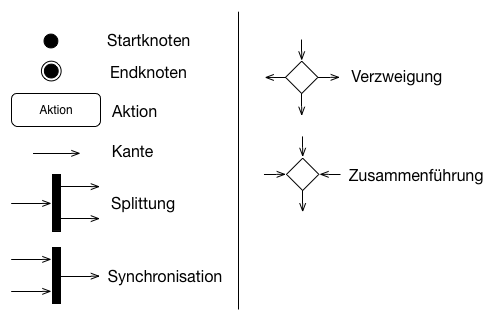
\includegraphics[width=1\textwidth]{graphics/stateoftheart/Activity_Elemente}
  \caption{Basis Elemente eines Aktivitätsdiagramm}
\end{figure}
%Quelle OMG Unified Modeling LanguageTM (OMG UML), Version 2.5
An Activity is a kind of Behavior (see sub clause 13.2) that is specified as a graph of nodes interconnected by edges. A subset of the nodes are executable nodes that embody lower-level steps in the overall Activity. Object nodes hold data that is input to and output from executable nodes, and moves across object flow edges. Control nodes specify sequencing of executable nodes via control flow edges. Activities are essentially what are commonly called “control and data flow” models. Such models of computation are inherently concurrent, as any sequencing of activity node execution is modeled explicitly by activity edges, and no ordering is mandated for any computation not explicitly sequenced.\\
Activities may describe procedural computation, forming hierarchies of Activities invoking other Activities, or, in an object- oriented model, they may be invoked indirectly as methods bound to Operations that are directly invoked. Activities may be applied to organizational modeling for business process engineering and workflow. In this context, events often originate from inside the system, such as the finishing of a task, but also from outside the system, such as a customer call. Activities can also be used for information system modeling to specify system level processes.\\
\\
Activity Nodes\\
ActivityNodes are used to model the individual steps in the behavior specified by an Activity.\\
\\
Activity Edges\\
An ActivityEdge is a directed connection between two ActivityNodes along which tokens may flow, from the source ActivityNode to the target ActivityNod.\\

%Quelle http://www.uml-diagrams.org/shopping-process-order-uml-activity-diagram-example.html?context=activity-examples
\begin{figure}[hbt!]
 \centering
  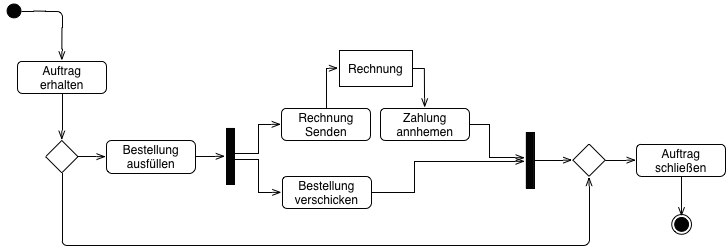
\includegraphics[width=1\textwidth]{graphics/stateoftheart/Activity_bsp}
  \caption{Beispiel für ein Aktivitätsdiagramm}
\end{figure}

\subsection{OPC}
OLE for Process Control\\
Object Linking and Embedding for Process Control (OPC)\\
%TODO OPC
XML, nur für Industrie.
\section{Fazit}
%
% Chapter3

\chapter{Konzept} \label{chapter:architecture}
Die Abfolge der Arbeitsschritte für die modellbasierte Entwicklung der Steuerung einer Chargenprozessanlage sieht wie folgt aus.
\begin{figure}[h!]
		\centering
		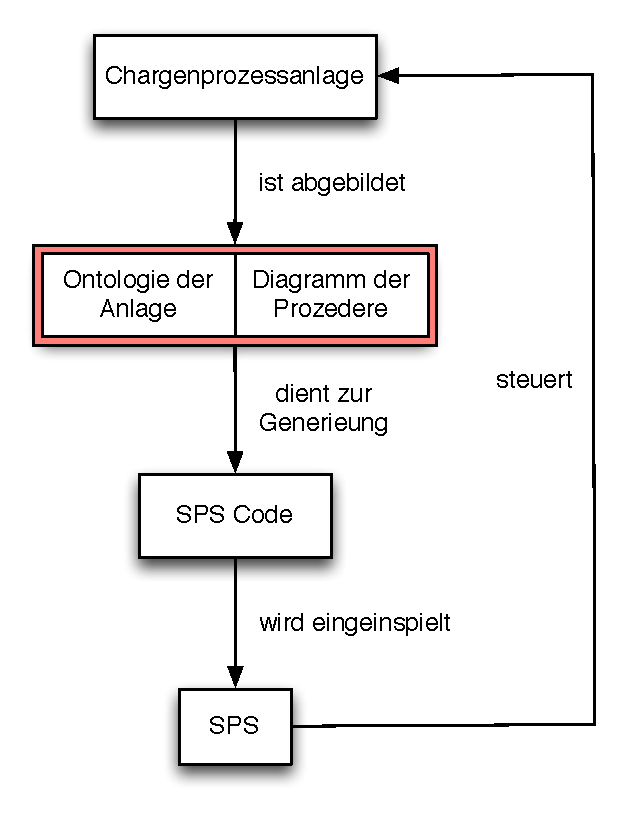
\includegraphics[width=0.37\textwidth]{graphics/konzept/konzept_new.pdf}
		\caption{Konzept für die modellbasierte Entwicklung der Steuerung}
		\label{fig:konz_konzept_new}
\end{figure} \\
\todo{modellbasierte entwicklung bei austausch/erweiterung}
Es beginnt mit einer Produktionsanlage, wobei es sich um eine Chargenprozessanlage handelt, die in einer Ontologie abgebildet wird. Die Ontologie und das Diagramm der Prozeduren beinhalten die nötigen Daten, die gebraucht werden, um im weiteren Schritt den Code für die SPS zu generieren. Dieser Code ist nach dem IEC 61512 Standard genormt. Nachdem der Code in die SPS eingespielt wird, kann die Chargenprozessanlage gesteuert werden. 
In diesem Kapitel wird jeder Schritt, der im Kreislauf von Abbildung~\ref{fig:konz_konzept_new} enthalten ist, genauer elaboriert und in Perspektive zu dem entwickelten Konzept gebracht.
\section{Produktionsanlage}
Für eine Anlage gibt es gewisse Parameter, die beim konzeptionellen Entwurf beachtet werden müssen. Für die gestellten Anforderungen sowie für die zukünftig darauf aufbauenden Projekte ist es unentbehrlich, dass diverse Redundanzen vorhanden sind. Eine Voraussetzung ist jedenfalls eine Vielzahl an Hauptleitungen. Durch diese kann erst ermöglicht werden, zwei Arbeitsschritte parallel auszuführen. Das noch folgende Vorhaben, einen Wegfindungsalgorithmus zu integrieren, ist obendrein nur nutzbringend, wenn mehrere, durch die Redundanz gebotene Wege zur Auswahl stehen. Ebenso ist die Disponibilität von mehr als einer Pumpe eine essentielle Bedingung. Dadurch kann die Anlage bei der Eventualität eines Ausfalls einer Pumpe diese vollständig kompensieren. Die Ansteuerung jeder einzelnen Funktion muss somit stets von geringstenfalls einer anderen Pumpe durchführbar sein. Zudem ist es vorgesehen, auf ausgewählten Routen die Steuerung mit Hilfe der Schwerkraft durchzuführen.\\

%Ein Ziel der Anlage muss sein, eine möglichst hohe Effizienz mit der modellbasierten Entwicklung zu erreichen.\\


\begin{figure}[h!]
		\centering
		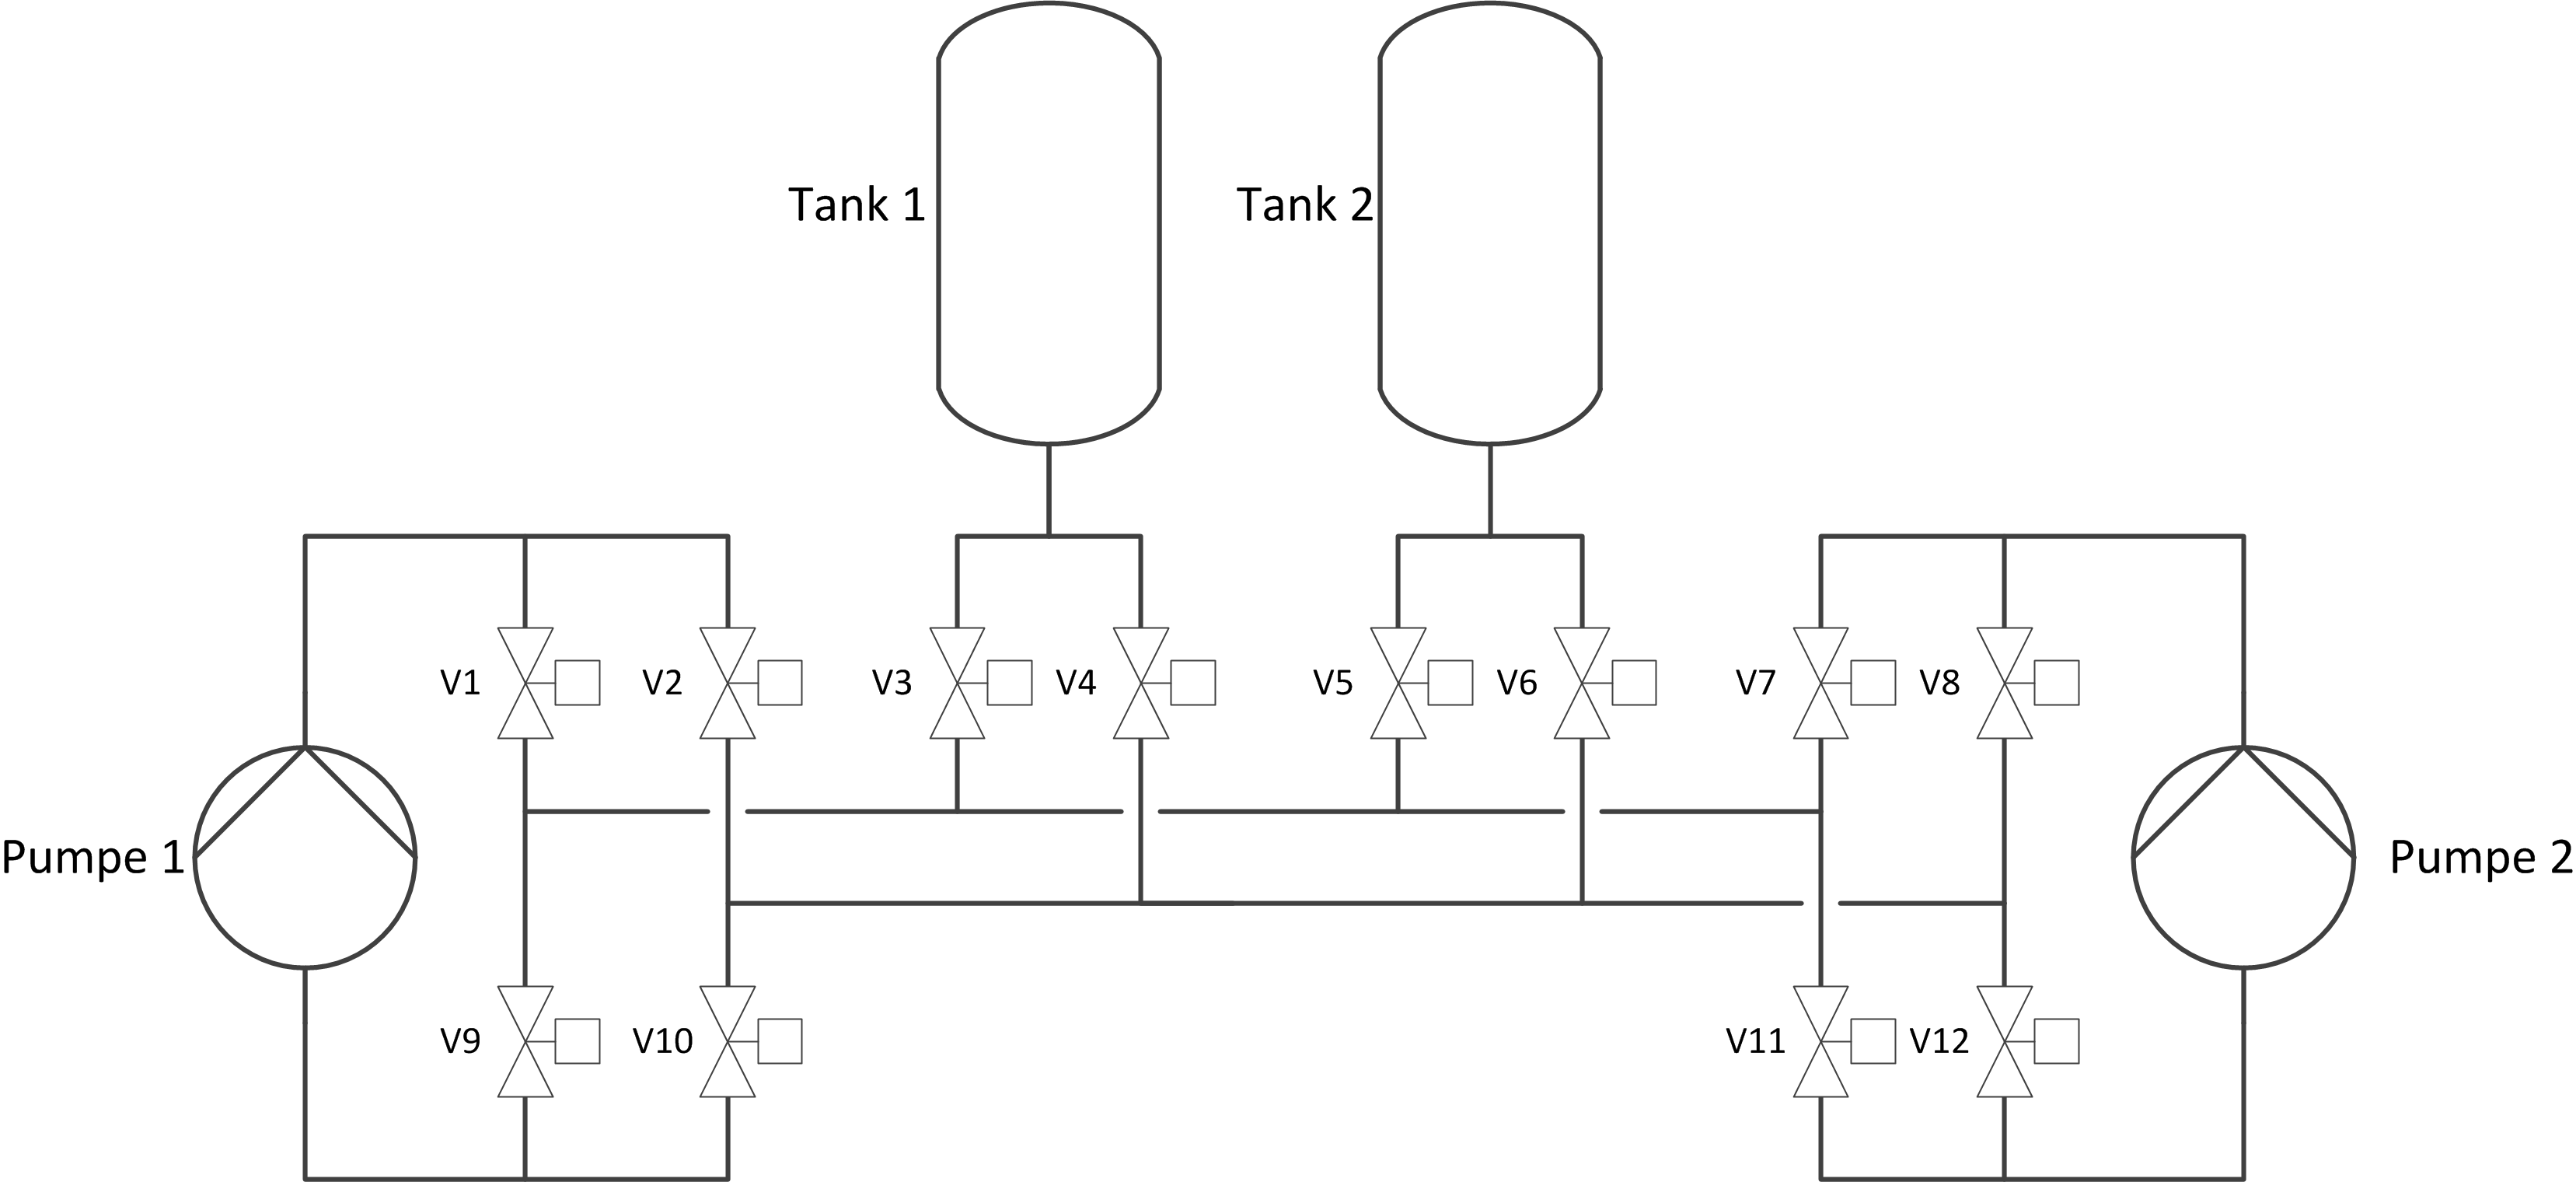
\includegraphics[width=1\textwidth]{graphics/konzept/RI_K.png}
		\caption{Konzept einer Anlage mit Redundanzen}
\end{figure}
\section{Informationskonzept}
Die Informationen für die Codegenerierung benötigen einerseits einen Ontologie, zur Speicherung der Informationen der Produktionsanlagen, und andererseits ein Aktivitätsdiagramm. In diesem werden die gewünschten Prozeduren dargestellt, die später generiert werden sollen.
Die beiden sind von einander abhängig, denn die Namen, der von in der Ontologie erstellen Identitäten (Datensätze), werden den Namen des Aktivitätsdiagramms zugeordnet.
Mithilfe der Ontologie und des Aktivitätsdiagramms können die Informationen bereitgestellt werden, die für die Codegenerierung nötige sind.  

\subsection{Ontologie der Chargenprozessanlage}
Hierbei handelt es sich um die Speicherung der Daten der Produktionsanlage in einer Ontologie. Je genauer diese abgebildet ist, desto mehr kann automatisch generiert werden. Wenn zum Beispiel Maximal- und Minimalwerte einfließen, können diese berücksichtigt werden.
Eine Ontologie, die eine Chargenprozessanlage abbildet, kann folgendermaßen aussehen. 
\begin{figure}[hbt!]
 \centering
  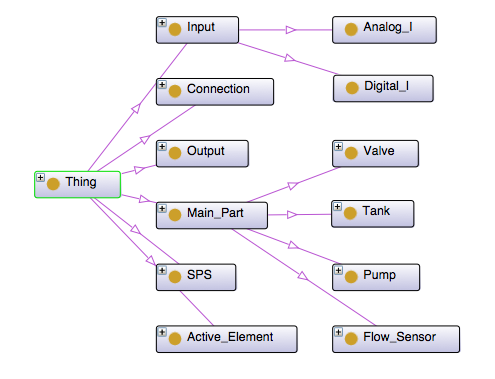
\includegraphics[width=0.6\textwidth]{graphics/stateoftheart/Ontology_Aufbau}
  \caption{Aufbau einer Ontologie}
\end{figure}\\
%Die Verbindungen zwischen den Klassen (In Abbildung 3.2. die Vierecke)
\todo{Referenz rausnehmen?}
Damit bei der Codegenerierung ein hoher Automatisierungsgrad  erreicht werden kann, müssen möglichst viele Daten abgespeichert werden. In einer Ontologie können unteranderem Klassen (Classes), Eigenschaften von Klassen (Object Properties) und Verbindungen zwischen Klassen (Data Properties) definiert werden. Für genauere Erklärung einer Ontologie siehe Kapitel 2.3 \glqq Modellbasierte Entwicklung der Steuerung\grqq. Dies wird sich zu Nutze gemacht um die Produktionsanlagen sehr genau abzubilden. Damit die Codegenerierung best möglich umgesetzt werden kann, werden folgende Daten einer Chargenprozessanlage gebraucht:

\begin{itemize}
  \item Elektrische Elemente (Pumpe, Ventil, SPS)
  \item Nicht- Elektrische Elemente (Tank, Reaktor)
  \item Eigenschaften der Elemente (Maximal- Minimalwert, Analog/Digital)
  \item Verbindung zwischen den Elementen (Eins-zu-Eins, Kreuzung)
\end{itemize}

\textbf{Elektrische Elemente}\\
Diese Kategorie beinhaltet alle Elemente die einen I/O Port in einer SPS brauchen, um mit Strom versorgt und angesprochen zu werden. Darunter können zum Beispiel eine Pumpe, ein Ventil, jegliche Art von Sensor aber auch ein Rührstab oder ein Heizelement fallen. \\\\
\textbf{Nicht- Elektrische Elemente}\\
Hierbei werden alle Elemente beschrieben, die keinen I/0 Port in der SPS haben, aber wichtig für die Chargenprozessanlage sind. Somit fällt zum Beispiel ein Tank und Reaktor in diese Gruppe. Zusätzlich könnten auch die Rohrleitung abgebildet werden.\\\\
\textbf{Eigenschaften der Elemente}  \\
Diese Kategorie kann beliebig genau behandelt werden, wobei ein gutes Mittelmaß gefunden werden sollte. Grundsätzlich ist jede zusätzliche Information eines Elements wertvoll für die Codegenerierung, allerdings kann eine zu detailreiche Beschreibung umständlich bzw. aufwändig auszuwerten sein und keinen wirklichen Nutzen bringen.
So sind zum Beispiel Maximal- und Minimalwerte sehr sinnvoll, aber die Abmessung der jeweiligen Elemente überflüssig. Weitere wertvolle Eigenschaften sind die Übertragungsarten (Analog oder Digital) und der Standard Zustand von elektronische Elementen, ob z.B. das Ventil offen oder zu ist wenn kein Strom fließt.   \\\\
\textbf{Verbindung zwischen den Elementen}  \\
Dabei werden die Verbindungen (z.B. mit Rohren) der Chargenprozessanlage zwischen den Elementen beschrieben. 
%Es kann sich entweder um eine Element zu Element (Eins-zu-eins) Verbindung handeln oder einen Kreuzung, also mehr als zwei Elemente miteinander.
%Es kann entweder eine Eins-zu-eins Verbindung sein oder eine Kreuzung, das heißt es sind mehr als zwei Elemente miteinander verbunden. Eine wichtige Zusatzinformation ist die Richtung der Verbindung.
Hierbei kann es sich entweder um einen Eins-zu-eins Verbindung handeln oder um eine Kreuzung. Das heißt es sind mehr als zwei Elemente an einer Stelle miteinander verbunden. Eine wichtige Zusatzinformation ist die Richtung der Verbindung.

%3.32 Weg (Strom) (en: path, stream): Die Reihenfolge der Einrichtungen innerhalb einer Anlage, die zur Herstellung einer bestimmten Charge genutzt wird oder genutzt werden soll.

%3.37 Prozedur (en: procedure): Die Strategie, nach der ein Prozeß durchgeführt wird.
%ANMERKUNG: Im allgemeinen bezieht sich der Begriff auf die Strategie, nach der eine Charge in einer Anlage hergestellt wird. Er kann sich auch auf einen Prozeß beziehen, der nicht zur Herstellung eines Produkts dient, wie z. B. ein Reinigungsvorgang.

\subsection{Diagramm der Prozeduren}
Die Abbildung der Prozeduren ist die zweite Komponente der benötigten Informationen für die Codegenerierung. Es wird in einem Aktivitätsdiagramm nach der UML Norm erstellt. Dieses enthält die Prozedere, die später codegeneriert und im weiteren Schritt in der Chargenprozessanlage verwendet werden. \\\\
Jede Prozedur wird durch einen Start- und Endpunkt definiert. Dazwischen werden die Namen der Stationen geschrieben und diese mit Pfeilen verbunden. Das Diagramm für zwei Prozeduren könnte folgendermaßen aussehen: 
\begin{figure}[h!]
		\centering
		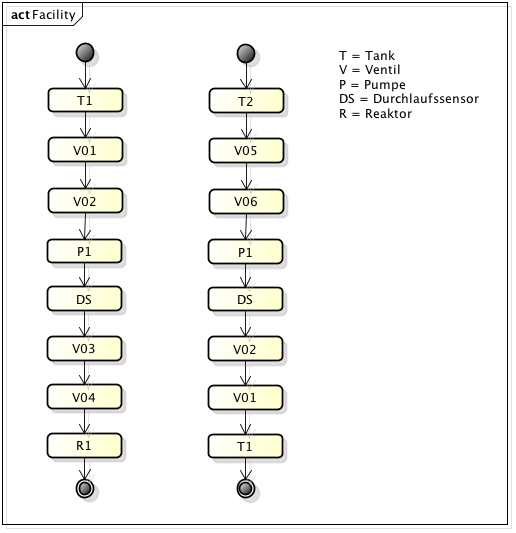
\includegraphics[width=0.7\textwidth]{graphics/konzept/UML_Activity.png}
		\caption{Abbildung der Wege mittels Aktivitätsdiagramm}
		\label{fig:konz_UML_Activity}
\end{figure}\\
In Abbildung~\ref{fig:konz_UML_Activity} ist das erste Element der „Prozedur 1“ ein Tank (T1), gefolgt von der Öffnung zweier Ventile (V1, V2) und der Inbetriebnahme der Pumpe (P1). Danach ist die Messung des Durchflusssensor (DS1) gefolgt von der Öffnung weiterer Ventile (V3, V4) mit dem Ziel im Reaktor (R1). 
Mithilfe einer solchen Folge kann der Ablauf einer Prozedur genau bestimmt werden, um bei der Codegenerierung diese erstellen zu können. 
\section{Codegenerierung}
\subsection{Phasen}
\subsection{Rezepte}

%
% Chapter4
\chapter{Implementierung} \label{chapter:thevetestcase}
\section{Modellierung der Anlage}
Für das Aufbauen einer Anlage, ist ein vorab überlegtes Konzept von großer Bedeutung. Mittels des Rohr- und Instrumentenfließschemas wird ein später noch des öfteren abgeändertes Abbild erstellt. Die in der Anfangsphase aufkommenden Änderungen ergeben sich angesichts der nur partiellen Implementierung der Anforderungen. Initial wird hoher Wert auf Redundanzen gelegt. Erst eine größere Anzahl an Bauteilen kann einen parallelen Ablauf mehrerer Arbeitsschritte ermöglichen. Durch die drei eingebauten Tanks und zwei Reaktoren, die mittels der drei Hauptleitungen verbunden sind, ist das Umfüllen zwischen zwei Tanks, sowie das gleichzeitige Befördern von Flüssigkeit vom dritten Tank in einen der Reaktoren möglich.\\

Die zwei Pumpen sind so platziert, dass bei einem eventuell auftretenden Defekt die andere Pumpe deren Aufgabe übernehmen kann. Arbeitsschritte können dadurch zwar nur noch sequentiell abgearbeitet werden, jedoch kommt es nicht gleich zu einem totalen Ausfall der Funktionalität der Anlage. Eine weitere Absicherung gegen möglich aufkommende Störfälle ist die Position der Tanks. Durch ihre Lokalisation an der höchsten Stelle der Apparatur besteht die Opportunität die Schwerkraft zu nutzen.\\

\begin{figure}[h!]
  \centering
  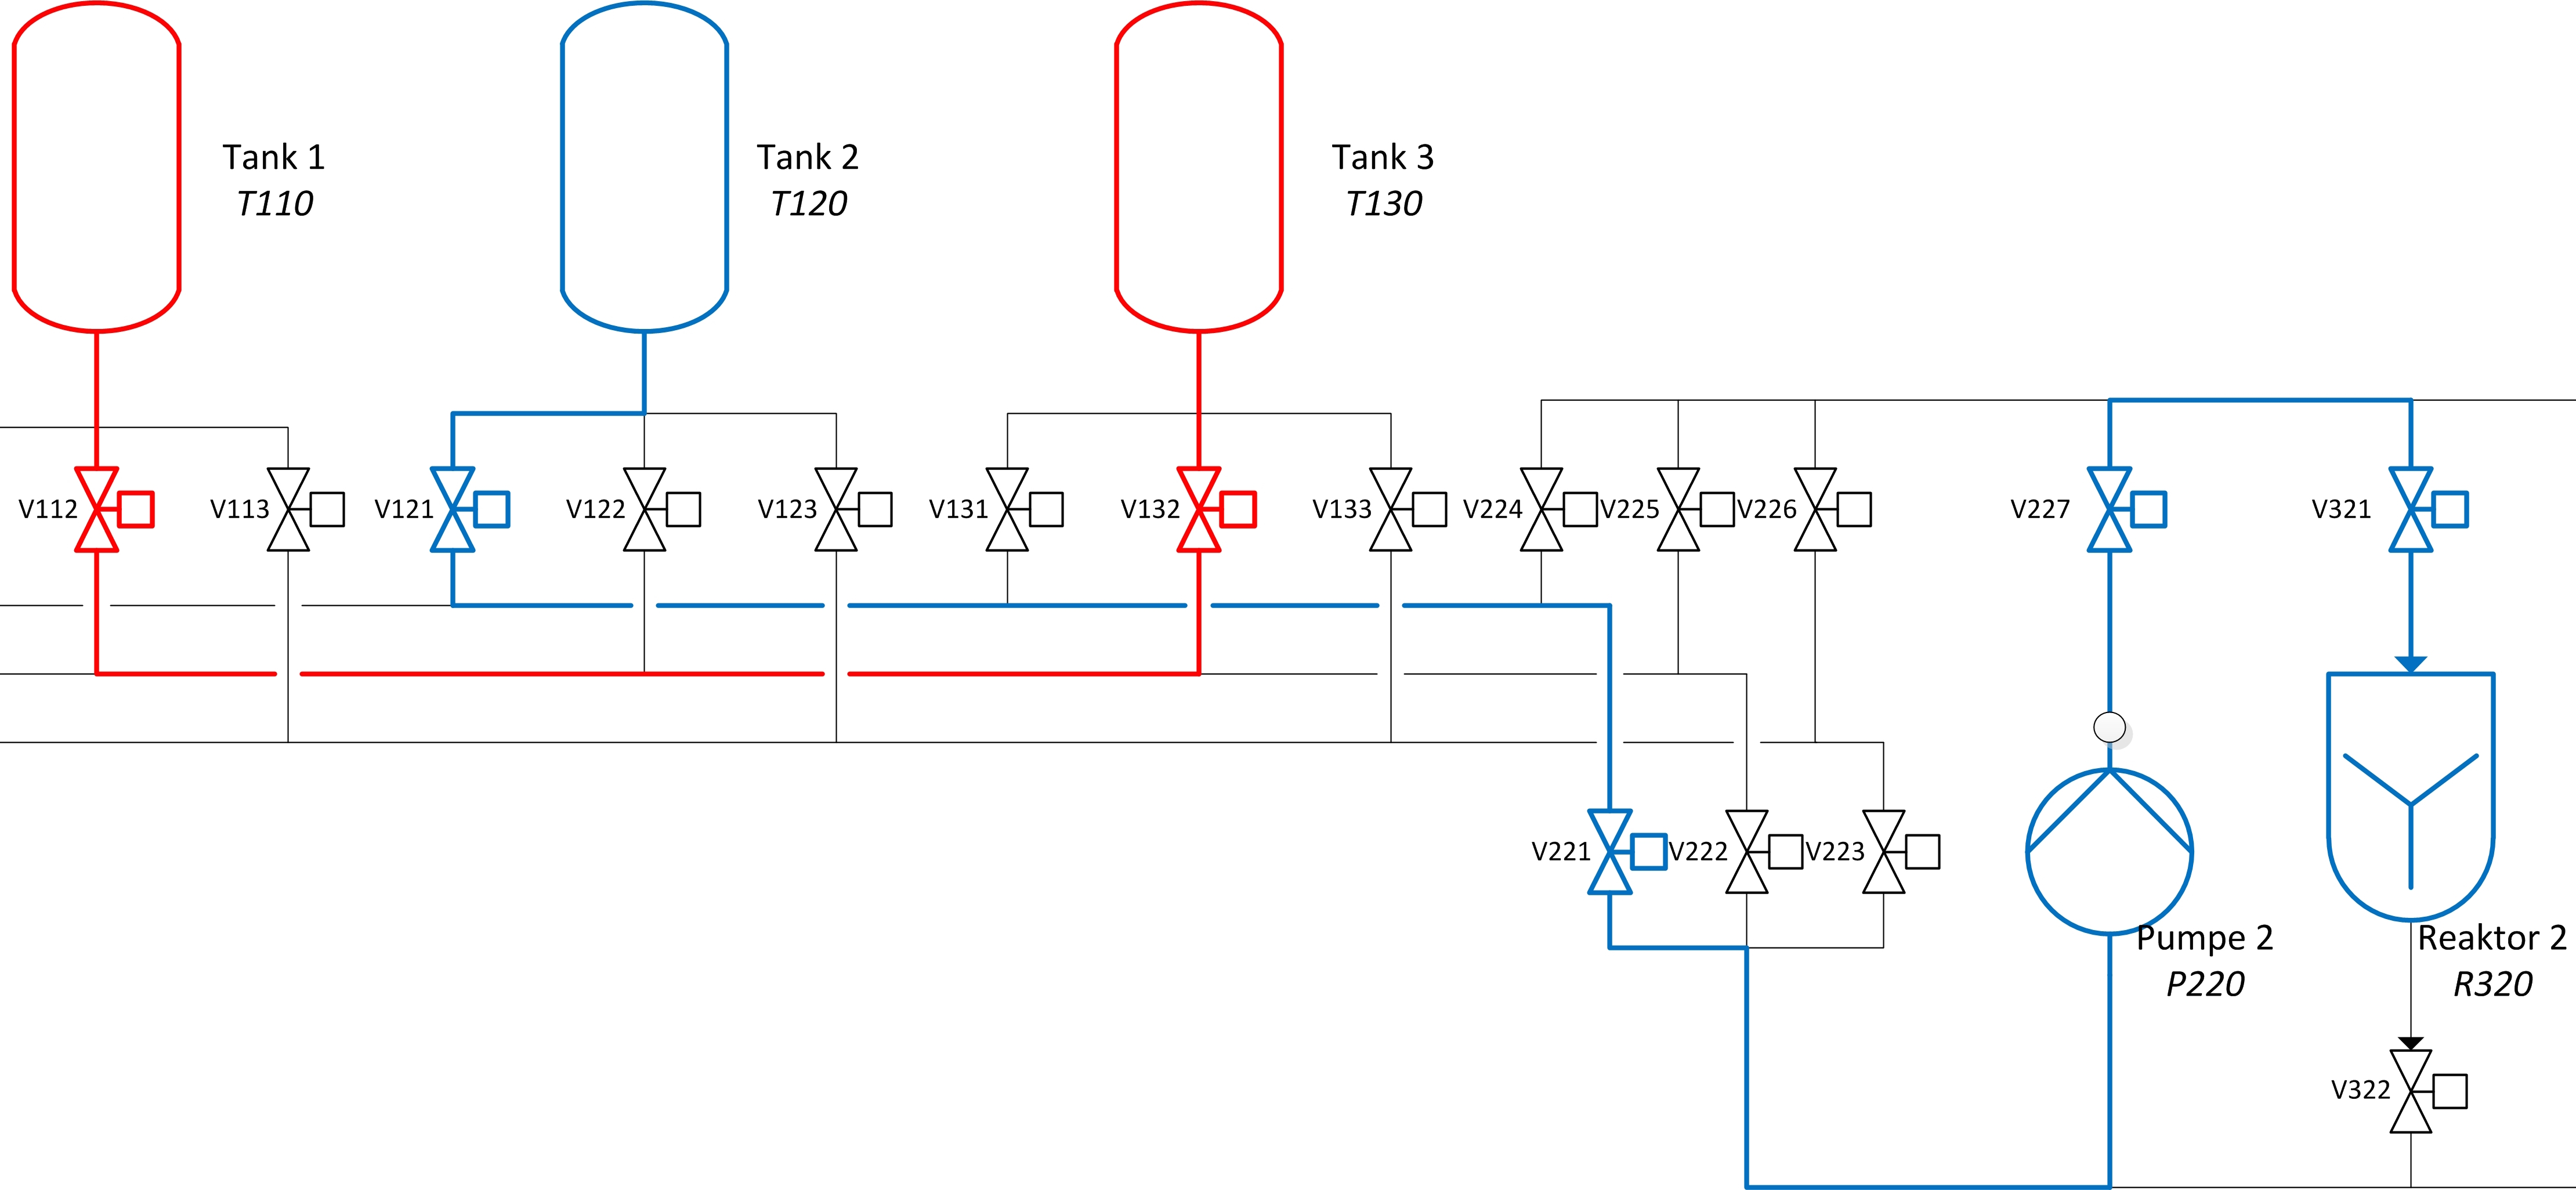
\includegraphics[width=1\textwidth]{graphics/implementation/RI_Impl_cropped.jpg}
  \caption{Mögliche Parallelität im RI ersichtlich}
\end{figure}

Jedes Ventil hat eine vorteilhafte Durchflussrichtung, die meistens mit einem Pfeil direkt auf dem Bauteil gekennzeichnet ist. Ganz abgesehen davon, ob es sich um ein Ventil handelt, welches im stromlosen Zustand geschlossen ist oder ob es ein schließendes Ventil ist, diese Vorgabe sollte stets eingehalten werden. Aspekte wie dieser haben in die Modellierung der Anlage selbstverständlich eingebaut zu werden.\\

\todo[inline]{BILD EINFÜGEN}

\begin{figure}[h!]
  \centering
  %\includegraphics[width=0.7\textwidth]{graphics/implementation/BILD}
  \caption{Ventil mit vorteilhafter Fließrichtung}
\end{figure}

Um in der Anlage befindliche Flüssigkeiten zu entfernen, muss ein eigens für den Auslass vorgesehenes Ventil installiert werden. Vorteilhafterweise handelt es sich bei der Position dieses Bauteils um den tiefsten Punkt der Apperetur. Alternativ dazu kann dieses auch direkt nach einer Pumpe montiert werden.

\section{Aufbau der Anlage}
Auf Basis des Rohr- und Instrumentenfließschemas kristallisiert sich eine exakte Anzahl an benötigten Bauteilen heraus. Für den noch bevorstehenden Aufbau der Anlage ist zu beachten, dass beim Auswählen der Einzelteile alles kompatibel sein muss. Nicht vorhandene Vereinbarkeit kann vor allem für diesen speziellen Anwendungszweck zu katastrophalen Auswirkungen führen, da einerseits mit Flüssigkeiten gearbeitet wird, sowie gleichzeitig stromdurchflossene Leitungen existieren. Eine Verbindung dieser genannten Komponenten hätte irreparable Schäden zur Folge. Im Rahmen einer übergeordneten Forschungsarbeit wurde diesem Projekt ein Budget von 6000 \todo{Euro} \euro \space zugesprochen. Die Auswahl der benötigten Teile hat verständlicherweise im Rahmen dieser beschränkten Geldmittel zu geschehen.\\
	
	Für einige verwendete Element gibt es spezifische Parameter, die auf jeden Fall einzuhalten sind:\\
	
	\textbf{Ventile:}\\
	Ein ausschlaggebendes Kriterium der verwendeten Ventile ist, dass sie in stromlosem Zustand geschlossen sind. Im Falle eines Ausfalls der Energieversorgung kann somit sichergestellt werden, dass sich alle Verbindungen aus Schutz vor Flüssigkeitsverlust schließen. Für die Funktion der Nutzung der Schwerkraft zum Umleiten von Flüssigkeiten ist auch relevant Ventile zu haben, die keinerlei Vordruck benötigen um den Durchfluss zu gewähren.\\

	\textbf{Tanks:}\\
	Abgesehen von einem für Testzwecke vernünftigen Füllvolumen ist es erforderlich einen Tank zu wählen, dessen Ausgang sich am niedrigsten Punkt befindet. Andernfalls kann man nur bedingt Nutzen aus der Schwerkraftsteuerung ziehen.\\
	
	\textbf{Pumpen:}\\
	Mit Hilfe eines Gleichstrom - Wandlers muss es möglich sein, die Pumpen mit dem zur Verfügung stehenden Ausgangstrom der SPS von 0 bis 10 Volt zu betreiben.\\
	
	\textbf{Rohre:}\\
	Die Rohre müssen jedenfalls dem Druck der Pumpen standhalten können. Desweiteren ist das exakt abzustimmende Einpassen in die Ventile, um Dichte gewährleisten zu können, ein wichtiger Parameter.\\

	Die bereits bei der Bestellung bekannten, tatsächlichen Maße der Bauteile, haben einen relevanten Einfluss auf den finalen Aufbau. Da es auch bei der Profilplatte physikalische Grenzen gibt, muss die endgültige Positionierung genauestens überlegt ausfallen. Der zukünftigen Vereinfachung des Aufbaus der Produktionsanlage halber, wurde daher projektintern beschlossen, ein kleines Modell der Apparatur zu erstellen. Da aus dem Rohr- \& Instrumentenfließschema keinerlei Information zur endgültigen Lokalisation der Bauteile ersichtlich ist, wird ein erster physikalischer Entwurf konstruiert. Mit Hilfe diesem können Abstände zueinander stehender Elemente deutlich gemacht werden. Realisiert wird der genannte Prototyp mit leicht zugänglichen Arbeitsmaterialien wie etwa Trinkhalme, Papier und Klebeband.\\
	
		\todo {Bild des Miniaturmodells}

	Für den tatsächlichen Aufbau ergibt sich günstigerweise die Möglichkeit, mechanische Anforderungen mit Hilfe der technischen Werkstätte abzuwickeln. Profilschienen, die als stabilisierendes Gerüst dienen, werden penibelst mit der Aluminiumsäge auf das gewünschte Maß geschnitten. Im späteren Verlauf werden diese samt den Tanks zum ersten aufgebauten Teil der Anlage. Für die Verbindung der Tanks, Pumpen, Ventile und Reaktoren dienen undurchsichtige Kunststoffrohre. Um gewährleisten zu können, dass die Verbindung absolute dicht ist, müssen die Rohre unbedingt gerade geschnitten sein. Abermals dürfen dafür Maschinen der mechanischen Werkstatt verwendet werden. Erst mit einer Bandsäge grob vorgeschnittene Rohrstücke werden in eine konventionelle Drehmaschine eingespannt. Mit einem scharf angeschliffenen Drehstahl ist es möglich, den unsauberen Schnitt absolut plan zu gestalten. Nachdem abschließend einzelne Komponenten noch entgratet werden, ist die Arbeit an den Rohren zur Verbindung getan.\\
	
	Verbundungen mit den ersten neun Ventilen der Hauptleitungen und den Tanks können ab sofort verlegt werden.\\
	
		\todo[inline]{Bild: Erster Aufbau (Tanks, Hauptpipes)}
		
	Das Einbauen der bestellten Pumpen gestaltet sich komplizierter als gedacht, da die ursprüngliche Bestellung einen Fehler beinhaltet. Nur eines der beiden gelieferten Modelle entspricht der gestellten Anforderung, was einschließlich der Rücksendung weitere wertvolle Zeit kostet. Unterdessen kann die zweite Pumpe verbaut werden. Funktionale Bauteile dieser Art sind bei der zeitgemäßen verfügbaren Leistung gut gedämpft. Angesichts der Tatsache, dass man mit dieser bis zu 30 Meter hoch pumpen könnte, befindet sich auf der Unterseite ein gummiertes Verbindungsstück, um bei Inbetriebnahme die stärksten Vibrationen abfangen zu können. Mit vom Profilschienen Schneiden übergebliebenen Reststücken wird eine Konstruktion gebaut, um die Höhe der Pumpe mit der der Rohre gleichzusetzen. Unmittelbar nach der Pumpe wird ein Durchflusssensor angebracht, der im späteren Verlauf des Projekts zur automatischen Steuerung beitragen soll.
	
	Abermals in der Werkstatt genauest zugeschnittene Profilschienen ergeben eine Konstruktion zur Aufhängung der Reaktoren. Das beste Beispiel der Bauteil-Positionsuntreue eines Rohr- \& Instrumentenfließschemas ist anhand des aufkommenden Arbeitsschritts zu sehen. Ursprünglich sind die beiden Reaktoren seitlich der restlichen Anlage platziert. Da es die Profilplatte aber nicht zulässt, da sie nur eine gewisse Breite hat, müssen diese in den Vordergrund geholt werden. Bei der Bauart der Reaktoraufhängung ist zu beachten, dass das größt möglich aufkommende Gewicht ausschließlich dort zustande kommen kann, da Reaktoren zum Mischen mehrerer Tankinhalte verwendet werden können. Diese Überlegung muss jedenfalls dazu beitragen, ausreichend Stabilität und Belastungsfähigkeit zu erlangen.\\
	
	Die bereits eingebauten Ventile besitzen jeweils zwei Phasen und eine Masse. Die Verkabelung selbst wird mit einem starren 3-Phasen-Kabel umgesetzt, da über eine flexibles Litzenverbindung nicht so viel Strom geleitet \todo{Stimmt das?}  werden sollte. Aus Gründen der Übersichtlichkeit wird jedes Kabel sowie Ventil beschriftet, um eventuell aufkommende Komplikationen zu unterbinden. In den Rillen der Profilschienen verlegt, werden alle mit Kabelbindern verbundene Leiter zur SPS zurückgeführt. Im späteren Verlauf eines Folgeprojekts soll eine Verlegung der SPS an die Unterseite des Tisches geschehen, weshalb es ausschlaggebend ist, alle Kabel mit einem deutlichen Übermaß zu schneiden. Die deutlich beschrifteten Kabel können anschließend der Funktionalität des jeweiligen Bauteils entsprechend in den dafür konzipierten SPS-Slot eingebaut werden.\\
	
	Mit dem Einbau der Füllstandssensoren in den drei Tanks sind die letzten Arbeitsschritte des physikalischen Aufbaus der Anlage getan.

\section{Phasen und Rezepte}
	Der Begriff Prozedur beschreibt das Zusammenfassen mehrerer Grundfunktionen einer Anlage, um einen Ablauf zu automatisieren. Das Gegenspiel zwischen der Software zenon und der SPS kann als sogenannte \glqq State-Machine \grqq \space betrachtet werden. Da eine SPS dem zyklischen Abarbeiten programmierter Funktionen unterliegt, ist es ein ständiges Nachfragen ob ein jeweiliger Zustand schon erreicht wurde. Durch global gesetzte Status kann so ein automatischer Wechsel der ausgeführten Funktionen erfolgen. Als Rezept wird das Aneinanderreihen mehrerer Prozeduren bezeichnet, um einen weiteren Schritt der Automatisierung zu gehen.\\

\begin{figure}[h!]
  \centering
  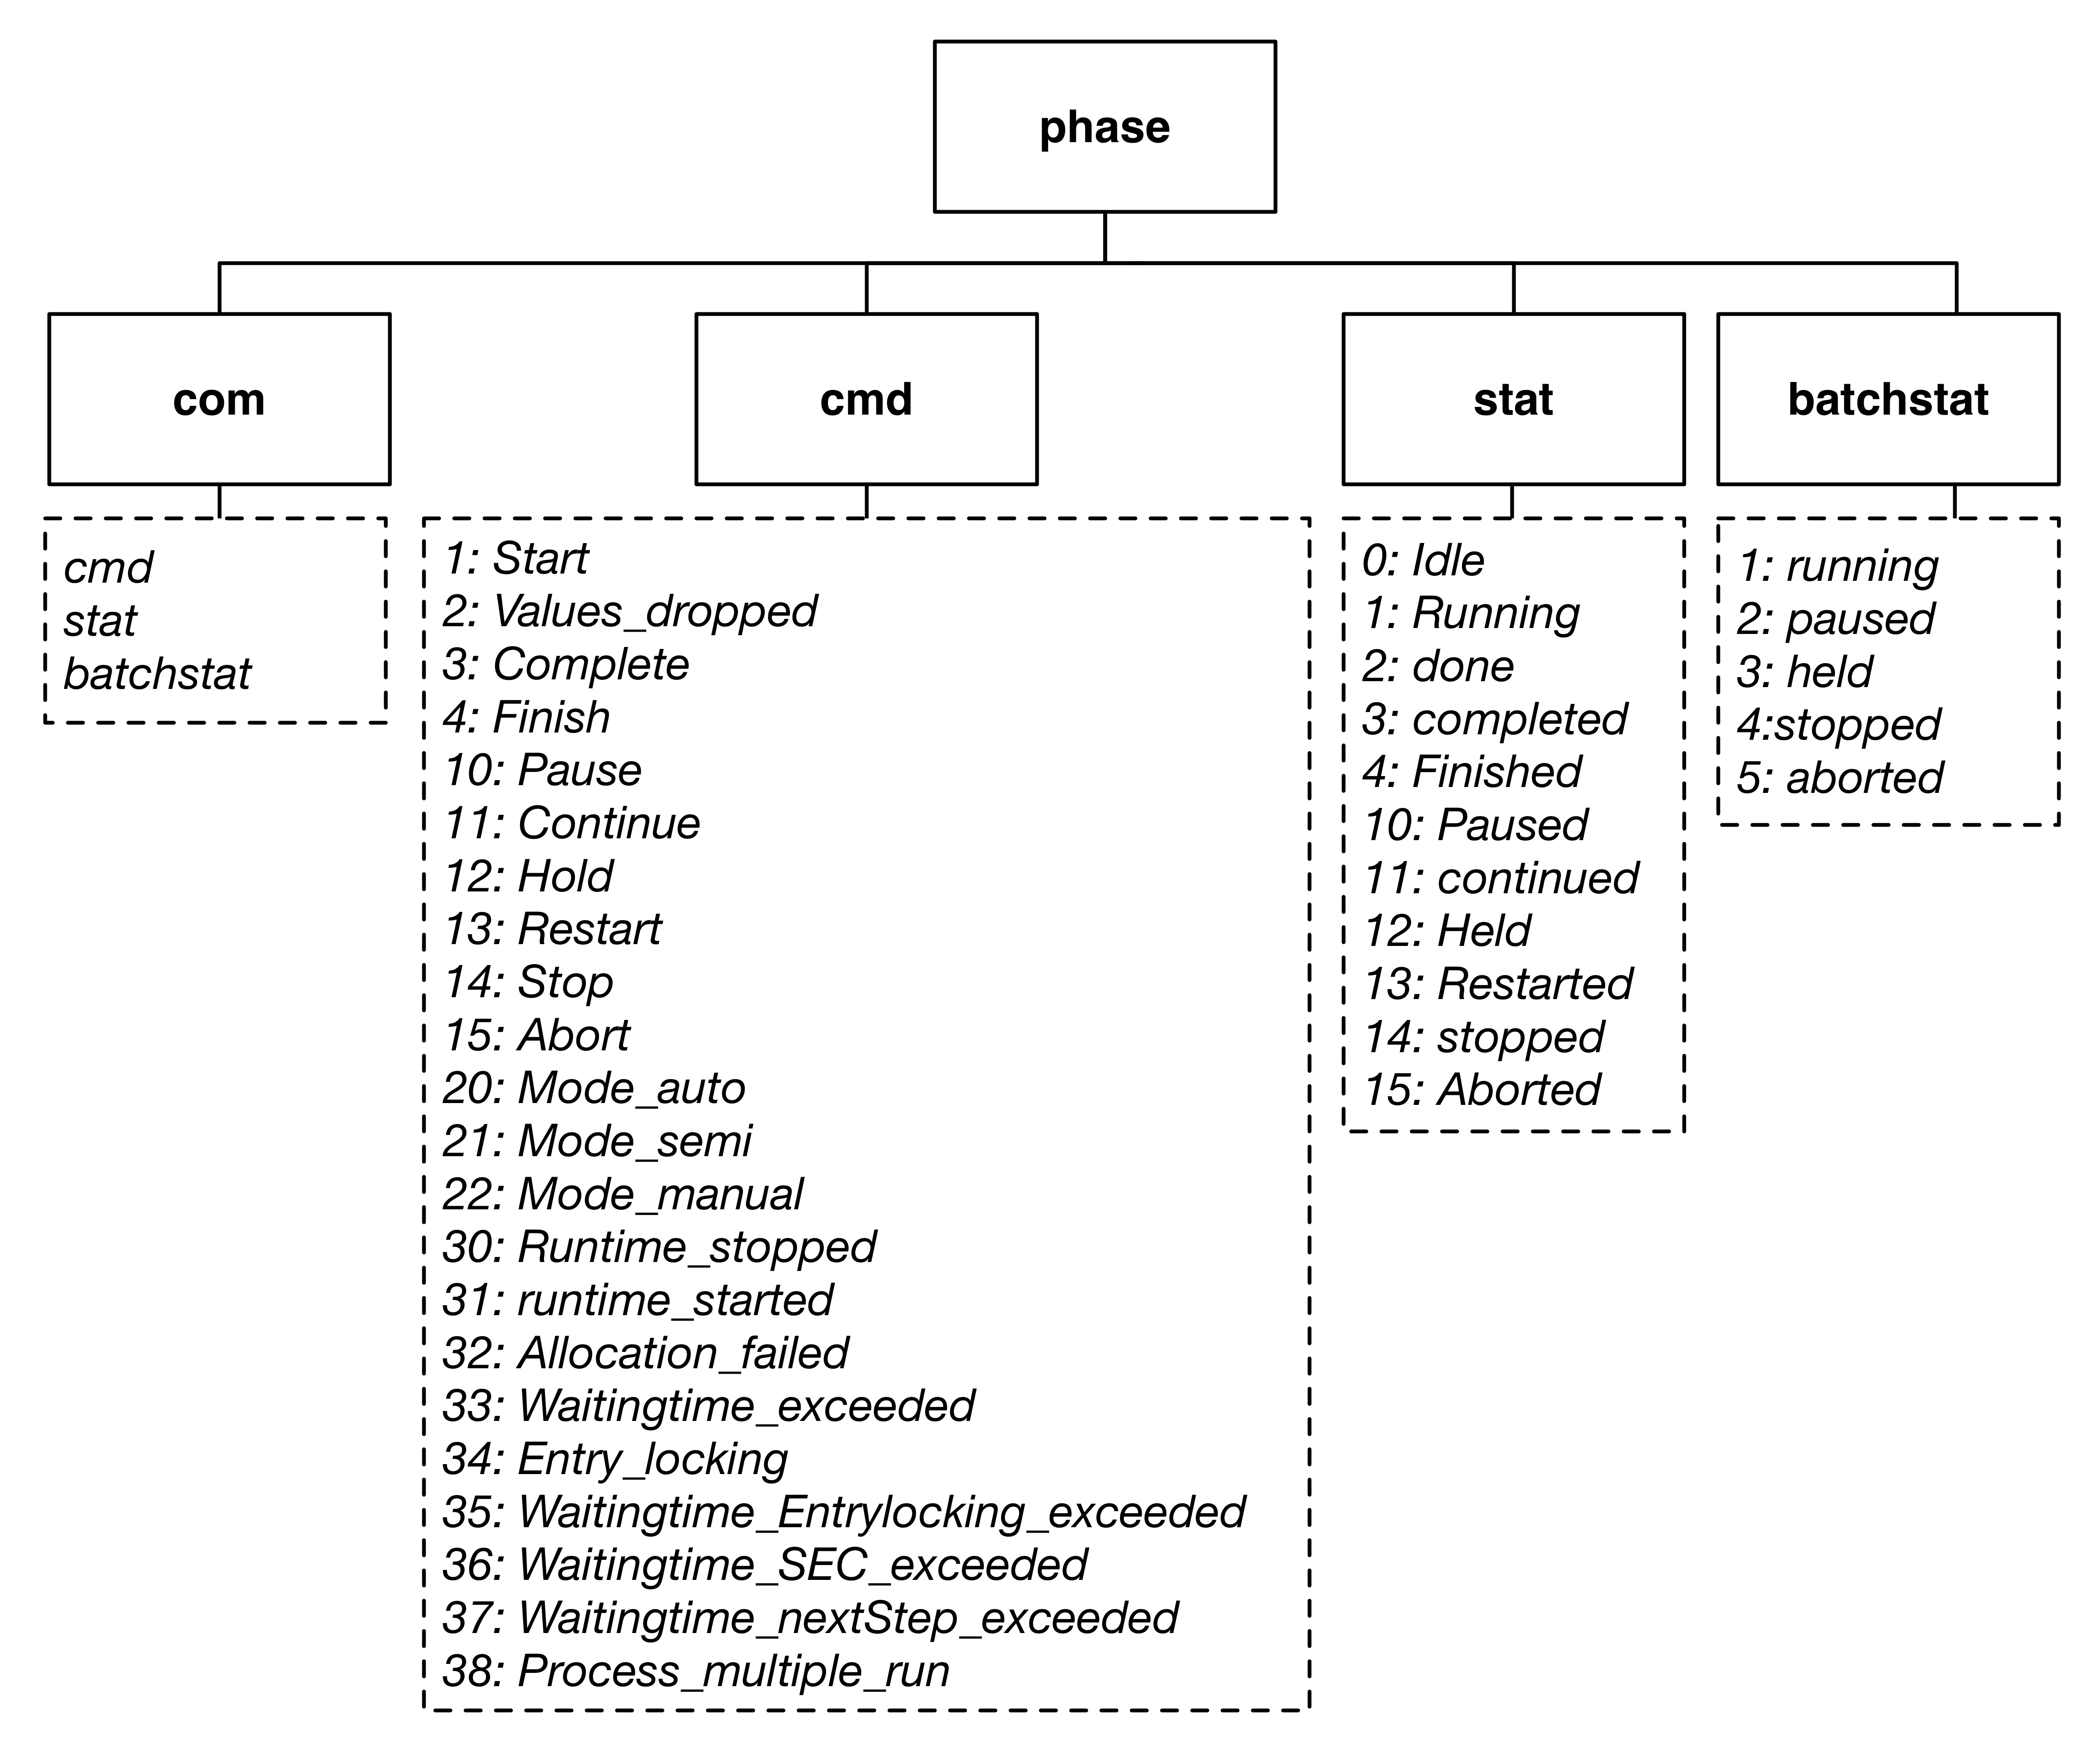
\includegraphics[height=0.6\textwidth]{graphics/implementation/Datentyp_Phase.jpg}
  \caption{Aufbau der Strukturvariable \glqq \textit{phase}\grqq}
\end{figure}
	
	Für die Kommunikation zwischen einer Prozedur bzw. eines Rezepts und der SPS stehen drei Variablen zur Verfügung
	
	\begin{itemize}
		\item Kommando: Sendet Befehle an SPS-Grundfunktion
		\item Status: Empfängt internen Status der SPS-Grundfunktion
		\item Batchstatus: Sendet internen Status des Rezepts zur SPS
	\end{itemize}

	Kommando trägt der SPS auf, was getan werden muss. Mit dem Status wird der Software zenon mitgeteilt, in welchem Stadium sich die Prozedur gerade befindet. Die Variable Batchstatus teilt mit, wo im gesamt abzulaufenden Programmcode sich die SPS gerade befindet.\\
	
	Um eine Prozedur in zenon zu konfigurieren, benötigt es eine ganze Anzahl an zu erledigenden Arbeitsschritten, die da wären:\\

	Initialisierend wird im Unterpunkt Batch Control ein neues Aggregat mit einer sich darin befindlichen neuen Grundfunktion (Prozedur) angelegt. Die Prozedur benötigt nun die zuvor erwähnten Kommunikationsvariablen Status, Command und BatchCommand. Zu beachten ist allerdings, dass es diese Strukturvariable bereits in der Form \glqq \textbf{name}.com.* \grqq \space gibt. Abermals untergeordnete Reaktionen werden mit den gewünschten Ereignissen befüllt, wobei wiederum zu beachten ist, dass diese den richtigen Variablen zugeordnet sein müssen.\\

	Weitere Arbeitsschritte werden mit mittels Zenon Logic abgearbeitet. Ein Hauptprogramm, welches zum Ausführen aller anderen Funktionen dient, wird angelegt. Aufgerufene Unterprogramme sind get\_cmd(), get\_batchstat(), die auszuführende(n) Prozedure(n) und send\_state() und müssen vor dem ersten Durchlauf des Hauptprogramms angelegt sein.\\
	
	\textbf{get\_cmd()}\\
	Null setzen (\glqq false\grqq \space setzen) aller Boolean-Werte, die einen Status repräsentieren, um alles zurückzusetzen, sowie durchgehen aller zur Auswahl stehenden Kommandos und setzen der Variable des zutreffenden Kommandos (\glqq true\grqq \space setzen).\\

	\textbf{get\_batchstat()}\\
		Zutreffender aktueller Status der Grundfunktion wird gesetzt.\\

	\textbf{Prozedur}\\
		Variablen bis zur Abbruchbedingung setzen\\

	\textbf{send\_state()}\\
		Globales Setzen des aktuellen Status
		
\begin{figure}[h!]
  \centering
  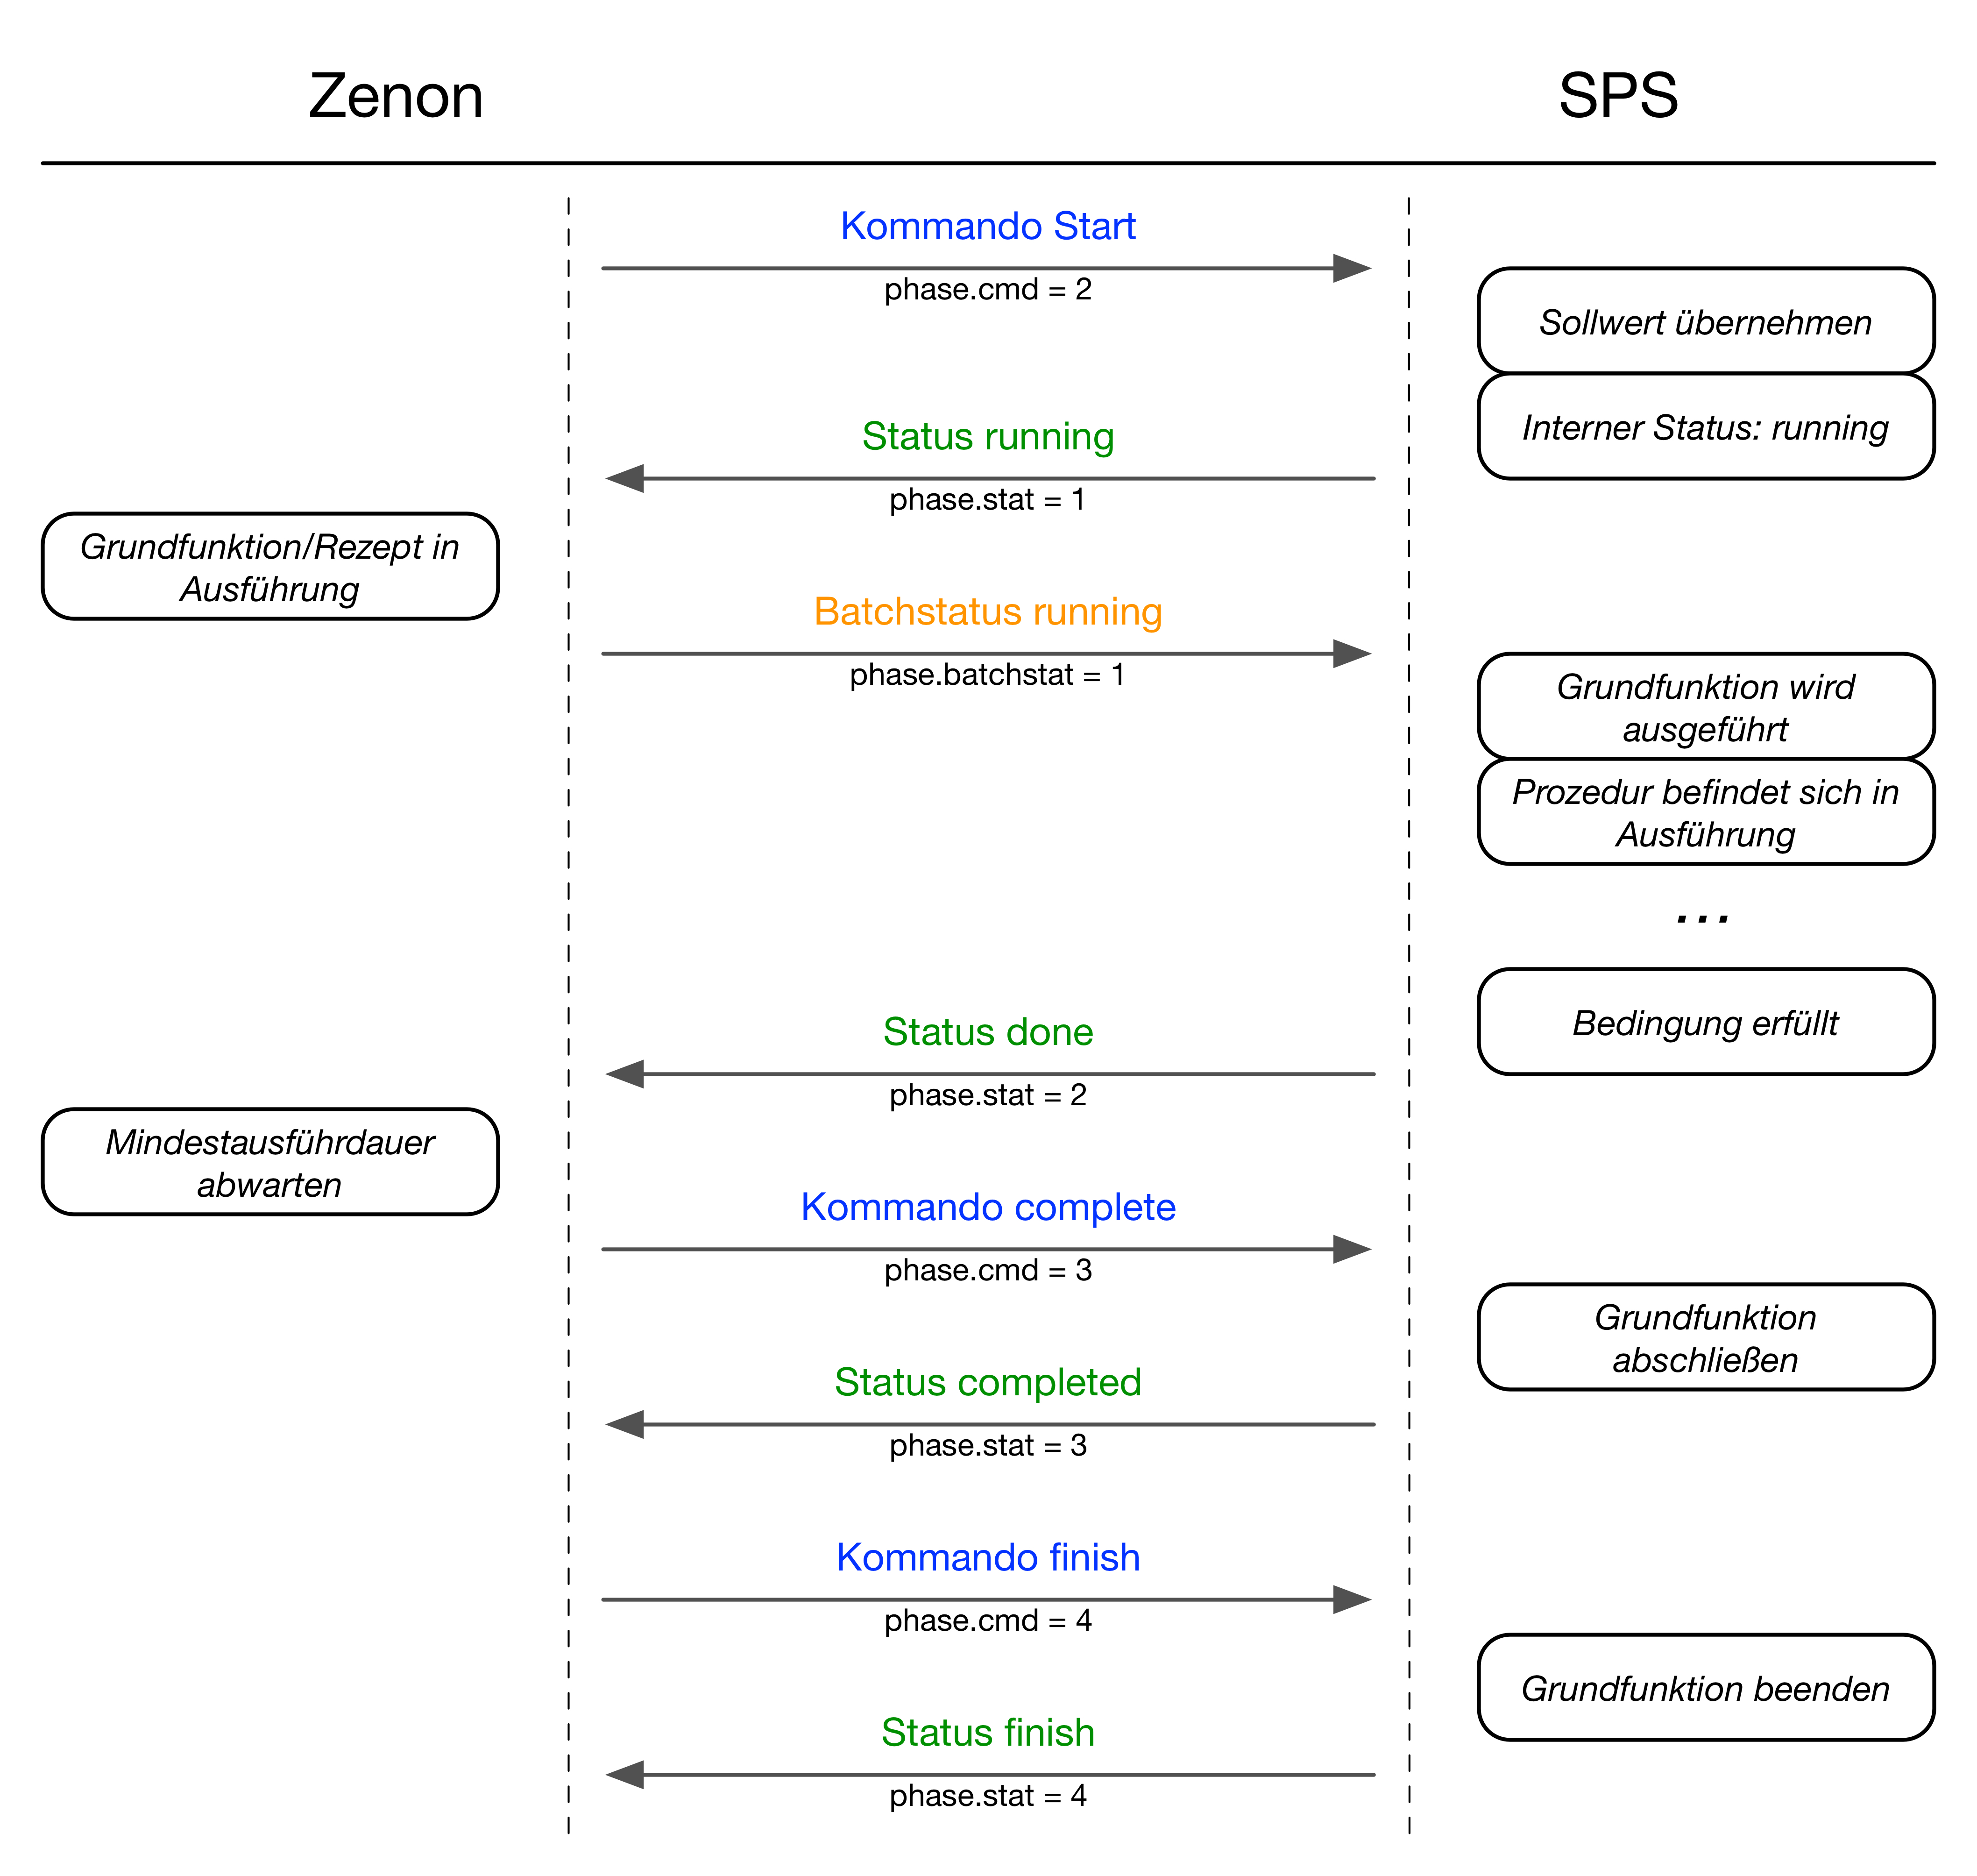
\includegraphics[height=0.95\textwidth]{graphics/implementation/StateMachine.jpg}
  \caption{Kommunikationsmodell von zenon und SPS}
\end{figure}

\section{HMI}
Für dieses Projekt wurde als SCADA System die Software zenon vorgegeben, daher wird das HMI in zenon Supervisor (zenons HMI Programm) umgesetzt.\\
\\
\textbf{Visualisierung}\\
In zenon wird eine Visualisierung \glqq Bild\grqq\space  gennant. Dieses kann mit vorgefertigten Elementen erweitert werden. 

Als Ausgangspunkt für die Visualisierung wurde das RI-Fließeschema zur Hand genommen. Aus diesem wurde die Anzahl der Elemente und die Grundstruktur übernommen. Als nächsten Schritt musste evaluiert werden, welche Inhalte des RI-Fließschemas für die Visualisierung relevant und welche Informationen nicht vorhanden waren.\\
\\
\textbf{Feldbuskonfiguration}\\
Um eine Visualisierung mit aktuellen Sensorwerten zu befüllen, wird eine Verbindung zur SPS benötigt. Diese Verbindung wird über das Teilprogramm zenon Logic (im weiteren nur noch Logic genannt) hergestellt.\\
\\
Als ersten Schritt, um in Logic eine SPS hinzuzufügen, muss im Unterpunkt \glqq Feldbuskonfiguration\grqq\space die Treibersoftware für die ADAM5550 SPS hinzugefügt werden. Daraufhin müssen alle Module, die an der SPS angebracht sind, in die Konfiguration hinzugefügt werden.\\%todo Position
\begin{figure}[h!]
  \centering
  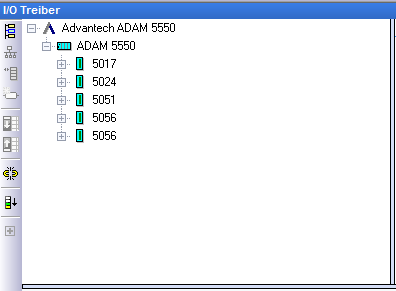
\includegraphics[width=0.7\textwidth]{graphics/implementation/Feldbuskonfiguration}
  \caption{Feldbuskonfiguration}%todo Grafik name
\end{figure}
\\
\textbf{Variablen}\\
In zenon können auf mehrere Arten Variablen erstellt werden. Damit diese für die Visualisierung und von Logic sichtbar sind, müssen sie als Globale Variable definiert werden. Der einfachste Weg dafür ist es, im Logic Variablenfenster, über den Reiter  \glqq Globale Variablen\grqq, die Funktion \glqq Variable hinzufügen\grqq\space aufzurufen.\\%todo Position
\begin{figure}[h!]
  \centering
  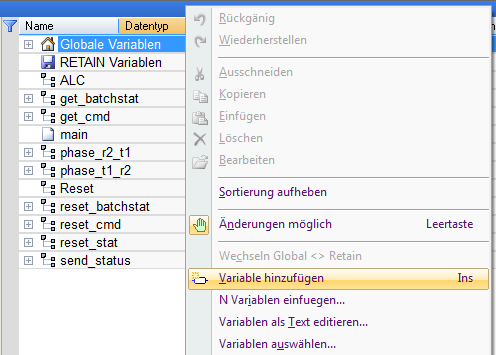
\includegraphics[width=0.7\textwidth]{graphics/implementation/Variablen}
  \caption{Variablen}%todo Grafik name
\end{figure}\\
Sobald alle Variablen erstellt sind, werden diese mit der Feldbuskonfiguration verknüpft. Durch diesen Schritt erhält man Zugang zu den an der SPS angeschlossenen Bauteilen.\\
\\

%Umrechnen von Sensorwerten: 
%Durchflusssensor Digital -> etwa 900 ticks pro Liter -> Timer bid 900 ticks -> Liter/min
%Füllstandsensor 4-20mA -> 4=voll, 20=leer -> Variablen/Tank Konfiguration -> Umrechnung 4=100, 20=0
%Ventilstatus 0/1 -> Variablen Konfiguration -> Extremwerte farblich markieren -> Ventil Elementfarbe nach Variablen Farbe
\textbf{Steuerung}\\
\\
Phase 1 Steuerung mittels Buttons\\
	Der erste Versuch war es die Steuerung mittels einfachen Buttons umzusetzen. Diese haben meist die in zenon vorhandene Funktion  \glqq Sollwert absetzen\grqq\space  verwendet, welche den Wert einer Variable ändert.\\
	So konnten alle Funktionen umgesetzt werden, dadurch erhielt das  \glqq Bild\grqq\space  jedoch viele Elemente die von der Eigentlichen Visualisierung ablenkten.\\
\\
Phase 2 Versteckte Buttons\\
	Um den Element-Overload zu verringern war der nächste Schritt die Button zu  \glqq verstecken\grqq\space  indem sie Transparent über die eigentlichen Elementen (beispielsweise ein Ventil) verschoben wurden.\\
	In der Visualisierung wurden nun weniger  \glqq unwichtige\grqq\space  Bausteine angezeigt, die Elemente waren jedoch immer noch da, wodurch die Größe (MB) der Visualisierung deutlich anstieg.\\
\\
Phase 3 Funktionale Elemente\\
	Der nächste schritt war es die nicht funktionalen Grafikelemente durch Buttons in Form der gewünschten Elemente zu ersetzten.\\
\\
\textbf{Rezepterstellung}\\
%todo Rezeperstellung

\section{Ontology}
Nachdem die Evaluierung der wichtigsten Aspekte im Kapitel Ontologie der Chargenprozessanlage in Hinsicht auf eine automatisierte Codegenerierung durchgeführt wurden, behandelt dieses Kapitel den Werdegang der Ontologie vom Ersten bis hin zum Finalem Design.\\
\\
Das Ziel der Ontologie ist es, die im laufe dieses Projekts aufgebaute Anlage in einer Art und Weise abbilden zu können, die es erlaubt daraus eine automatisierte Codegenerierung durchzuführen und dabei auf einem Abstraktionslevel zu bleiben um einen Großteil an in der Industrie vorkommenden Produktionsanlagen abbilden zu können.\\
\\
Da es den Rahmen dieser Arbeit sprengen würde, auf jeden einzelnen Gedankengang in der Erstellung der Ontologie einzugehen, werden nur die großen Revisionen der Ontologie genauer beschrieben.\\
\\
Zu aller erste werden alle Bauteile der Anlage in Kategorien eingeteilt.\\
Tanks, Reaktoren und Pumpen sind die Hauptelemente dieser Anlage und werden deswegen auch in einer Gruppe zusammengefasst. Neben ihnen gibt es eine Gruppe an Bauteilen die etwas tun, hierzu gehören die Ventile, Sensoren, Heiz- und Rührstäbe. Die restlichen Elemente der Anlage sind Statische Objekte die einen Nutzen besitzen, jedoch keine Arbeit erledigen, daher fallen diese zusammen unter die Kategorie von Passiven Elementen. Zu diesem Zeitpunkt sind dies nur die Rohre.\\
Eine Ausnahme dieser Gruppen ist die SPS welche etwas tut, daher an sich in Kategorie 2 Fallen würde, aber nicht direkt Teil der Anlage ist und daher auch als einzelstehendes Objekt einen Platz in der Ontologie findet.

\begin{figure}[hbt!]
  \centering
  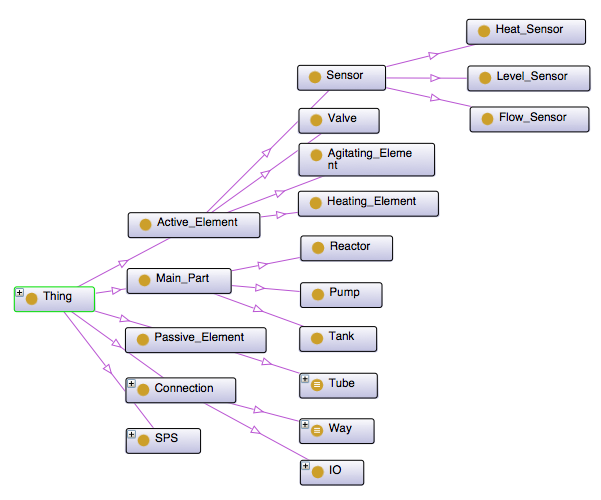
\includegraphics[width=0.6\textwidth]{graphics/implementation/Ontology_v1}
  \caption{Erste Version der Ontologie}
\end{figure}

Verbindungen zwischen 2 Klassen werden normalerweise mit einer Objekt Eigenschaft dargestellt, da eine Verbindung zwischen 2 Bauteilen aber eine andere Information als die Verbindung zwischen einer SPS und einem Bauteil enthält, gibt es die Kategorie Connections mit den Klassen “Weg” und “IO”.

Kurz zusammengefasst können die Kategorien wie folgt beschreiben werden\\
Main\_Part:\\
	Dies sind alle Elemente die subjektiv als Hauptelemente bezeichnet werden.\\
Active\_Element:\\
	Jene Bauteile die etwas tun - Aktuatoren, Sensoren\\
Passive\_Elements:\\
	In der Anlage verbaute teile die keine Arbeit verrichten.\\ 
Connection:\\
	Verbindungsarten zwischen den einzelnen Bauteilen\\
\\
Mit dieser Ontologie ist es grundsätzlich möglich die Anlage aus Kapitel 4.2 abzubilden, jedoch finden sich einige Inkonsistenzen die die automatisierte Codegenerierung erschweren wenn nicht sogar unmöglich machen würden.\\
\\
Nun wird die erste Version der Ontologie, in Hinsicht einer automatisierten Codegenerierung, evaluiert und dementsprechend umgebaut.\\
Die Kategorien werden im nächsten Schritt genauer definiert um eine Konsistenz in die Ontologie zu bringen.\\
\\
Die definition von \glqq Active\_Element\grqq\space ist in Grunde richtig, nur beinhaltet diese die SPS was nicht der Fall sein soll. Daher wird die Definition auf \glqq Elemente die mit einer SPS (I/O) verbunden sind\grqq\space geändert. In diese Kategorie fallen nun die Elemente der Ersten Version ohne SPS und auch die Pumpe hinein.\\
\\
Die nächste Kategorie die bearbeitet wird ist \glqq Main Part\grqq\space. Die Definition in dieser Gruppe ist noch sehr grob definiert und lässt eine Subjektive Gruppierung zu, daher muss die Definition von Grund auf geändert werden ohne Bauteile die zurzeit Enthalten sind auszuschließen. Die passende Interpretation ist \glqq Elemente mit mindestens 2 Ein bzw. Ausgängen\grqq\space. Durch diese Änderung fallen nun auch die Ventile in die Gruppe \glqq Main Part\grqq\space.\\
\\
Um Ein-/Ausgänge besser zu definieren wird die Gruppe \glqq Connection\grqq\space verändert. Die Klasse \glqq I/O\grqq\space wird heraus genommen da man diese genauer beschreiben muss. Dadurch enthält \glqq Connection\grqq\space nur noch Verbindungen zwischen Bauteilen, welche nur noch Ein-/Ausgänge sein können.\\
\\
Die Kategorie \glqq Passive Element\grqq\space wird komplett entfernt da sie keine Relevanten Information enthält.

\begin{figure}[hbt!]
  \centering
  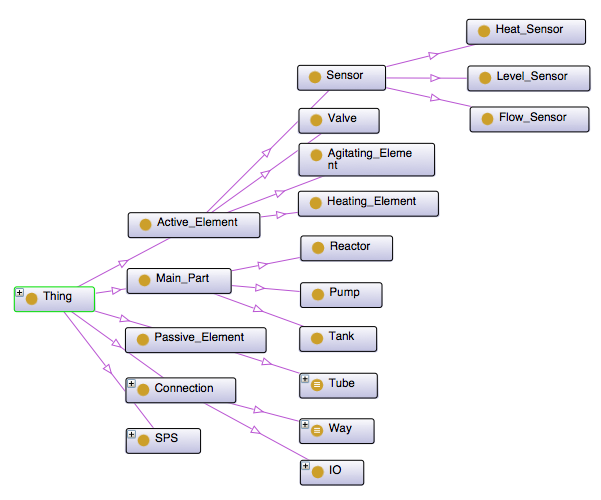
\includegraphics[width=0.6\textwidth]{graphics/implementation/Ontology_v2}
  \caption{Erste Überarbeitung der Ontologie}
\end{figure}

Von diesem Punkt aus wird die Ontologie nur noch verfeinert und nicht mehr großartig an der Struktur gearbeitet.\\
Die Klasse SPS wird, um Konsistenz in die Namen zu bringen, in die Englische Bezeichnung PCL umbenannt. 

\begin{figure}[hbt!]
  \centering
  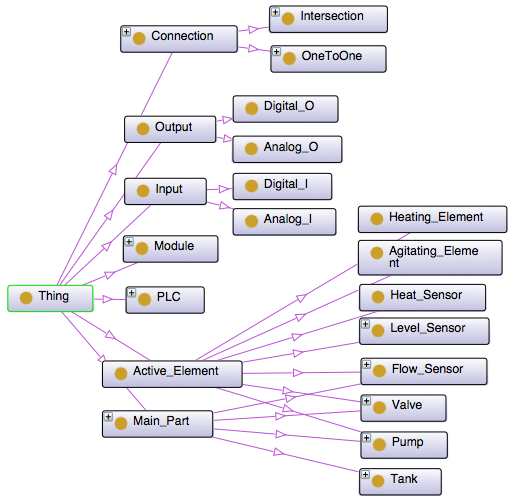
\includegraphics[width=0.6\textwidth]{graphics/implementation/Ontology_final}
  \caption{Finale Version der Ontologie}
\end{figure}

\textbf{Object Properties}\\
\\
Nachdem die Klassenstruktur feststeht, müssen als nächstes die Relationen bestimmt werden.
\begin{table}[h]
\centering
\begin{tabular}{l|l|l}
\textbf{Name} & \textbf{Domain} & \textbf{Range} \\ \hline
hasActiveE    & Input, Output   & Active\_Element \\ \hline
hasConnection & MainPart        & Connection      \\ \hline
hasIO         & Module          & Input, Output   \\ \hline
hasModule     & PLC             & Module          \\ \hline
isIncludedTo  & Tank            & Active\_Element \\ \hline
isConnectedTo & Connection      & Connection                            
\end{tabular}
\end{table}
\\
\textbf{Data Properties}\\
TODO
\section{Aktivitätsdiagramm}
TODO
\section{Codegenerierung}

TODO%
% Chapter5

\chapter{Evaluation} \label{chapter:evaluation}

%Einleitung + Aufgabenstellung
%3 Absätze mit länge halbe - 1 1/2 Seiten 
%Fragen werden beantwortet
%warum hats funktioniert oder warum hat es nicht funktioniert-> Begründung


%Mit welchen Technologien ist die Implementierung von Code einer SPS einer Chargenprozessanlage automatisierbar?

%Wie genau muss die Chargenprozessanlage abgebildet werden um einen Codegenerierung zu ermöglichen? 

%Welche Funktionalität kann durch die modellbasierte Entwicklung der Steuerung abgedeckt werden?

%Wie ausführlich funktioniert die Integrierung der Codegenerierung in die Software „zenon“ von COPA- DATA? 

Das Projekt Batch\_it hat sich zum Ziel gesetzt eine modellbasierte Entwicklung der Steuerung umzusetzen, wobei der erste Schritt die Konzeptionierung und der Aufbau einer Laboranlage war. Als weiteres sollte für diese eine Steuerungsapplikation mit Visualisierung mithilfe der Software zenon erstellt werden. Im letzten Schritt sollte die modellbasierte Entwicklung der Steuerung umgesetzt werden. Hierzu wurde eine Ontologie benötigt, welche die Laboranlage abbildet, und ein Aktivitätsdiagramm, welches die Prozeduren definiert. Anhand dieser Daten sollte eine Codegenerierung für die Steuerung der Anlage implementiert werden. \\\\
Die Modellierung der Chargenprozessanlage wurde mit Redundanzen versehen, um weiterführende Projekte zu unterstützen, und in einem Umfang erstellt, der die zu Verfügung gestellten Geldmittel nicht übertraf. 
%Die Modellierung der Chargenprozessanlage wurde mit Redundanzen versehen, um eine Laboranlage zu schaffen, die es ermöglicht moderne Ansätze in der Anlagen- und Verfahrenstechnik zu testen.
Die Auswahl der Bauteile war kein einfacher Prozess, da einige Parameter wie das Budget, die Kompatibilität und Verfügbarkeit beachtet werden mussten. So wurden die Rühr- und Heizelemente, die für die Reaktoren geplant waren, weggelassen, da diese zu teuere gewesen wären. Auch bei den Füllstandssensoren mussten Abstriche gemacht werden, da diese für alle Reaktoren und Tanks das Budget gesprengt hätten.
Der Aufbau der Anlage war eine langwieriger Aufgabe, die allerdings durch das Miniaturmodell beschleunigen werden konnte, da die Platzierung der Teile schon im Vorhinein überlegt werden konnte. Das Zuschneiden der Rohre musste sehr genau durchgeführt werden, da bei kleinen Abweichungen die Verbindungen schief gewesen wären. Schlussendlich konnte der Aufbau allerdings vollständig und erfolgreich abgeschlossen werden. \\\\
Die Visualisierung mithilfe von zenon konnte unproblematisch umgesetzt werden, da Vorkenntnisse mit der Software vorhanden waren. Bei dem Verbinden von \ac{SPS} und zenon stand der benötigte Treiber nicht zur Verfügung. Nachdem mit dem Hersteller der \ac{SPS} Kontakt aufgenommen wurde, konnte diese Problem gelöst werden. Das Einfließen lassen der Daten sowie die Steuerung über die Visualisierung funktionierte auf anhieb. Bei dem Erstellen von Prozeduren und Rezepten war ein umfangreiches Einlesen in die Thematik erforderlich.\\\\
%1. Frage
%Wie genau muss die Chargenprozessanlage abgebildet werden um eine Codegenerierung zu ermöglichen?
Die Genauigkeit der Abbildung der Chargenprozessanlage in der Ontologie ist hoch ausgefallen, allerdings sind für die automatische Entwicklung der Steuerung nicht alle Informationen verwendet worden. Zu den benötigten Daten haben die Elemente der Anlage (z.B. Tank, Sensor) sowie deren Attribute gehört. Dabei sind bei den Tanks Attribute wie z.B. Volumen verwendet worden und bei den elektrischen Elementen Maximum- und Minimumwerte sowie der Standard Zustand, ob z.B. das Ventil offen oder zu ist wenn kein Strom fließt. Da ein Aktivitätsdiagramm die Prozeduren definiert hat, wurde die Verbindungen, die abgebildet sind, nicht verwendet.
Die Ontologie ist detaillierter geworden als sie die Codegenerierung benötigt hätte, allerdings ist sie somit für Erweiterungen der Automatisierung in Zukunft vorbereitet. 
\\\\
%2. Frage
%Welche Funktionalität der Steuerung kann durch die modellbasierte Entwicklung der Steuerung abgedeckt werden?
Die Funktionalitäten der Steuerung konnten nicht alle vollkommen abgedeckt werden. Die Prozeduren wurden generiert und konnten in die Chargenprozessanlage steuern, aber  die Prozeduren abgedeckt werden. Das automatisierte Erstellen von Rezepten ist nicht erfolgreich gewesen, da das Integrieren in Batch Control nicht unterstützt wird. \todo{Beantworten}
\\\\
%3. Frage
%Wie ausführlich funktioniert die Integrierung der Codegenerierung in die Software zenon von COPA- DATA? 
Die modellbasierte Entwicklung der Steuerung wurde erfolgreich abgeschlossen. Es konnten aus der Ontologie und dem Aktivitätsdiagramm der Code für Prozeduren generiert und damit die Chargenprozessanlage gesteuert werden. Um den Code der Prozeduren in zenon zu integrieren ist allerdings eine Benutzerinteraktion benötig, weil das automatische Hinzufügen nicht möglich war. Zusätzlich gelang das Anlegen von Variablen inklusive Datentypen für die Elemente der Anlage in zenon. In zenon Logic können die Werte von Variablen mittels eines Scripts, welches beim Start ausgeführt wird, gesetzt werden. 
Die automatische Integrierung in Batch Control zum Erstellen der Rezepten wird von zenon nicht unterstützt und konnte deswegen nicht umgesetzt werden. 

%Das Erstellen der Ontologie für Chargenprozessanlagen war eine    

%Prozeduren generierbar durch Benuttzeraktion eingespielt werden 
%Für die abgebildenten Klassen kännen Datentypen erstellt werden. 
%Für die Elemente i der Anlage können Variablen mit entsprechenden Datentypen angelegt werden.
%Die automatische INtergrierung in Batch Control (GUI) zum Erstellen der Rezepte ist nicht unterstützt. 
%In Zenon Logic können von Variablen mittels einenm Sciripts beim start, mit ihnen im Modell abgebildetten Werte initialisiert werden.















%


\chapter{Zusammenfassung und Ausblick} \label{chapter:conclusion}
%was wurde in der Arbeit gemacht`? 
%Zusammenfassung was gemacht wurde, 1 Seite min
%was ist übrig geblieben ? -> Ausblick 
%Das wäre toll gewesen wenn man es lösen hätte können --> aus welchen gründen. 
%Wir haben nicht den wirtschaftlichen Aspekt 

%Das Diplomprojekt hat sich zur Aufgabe gemacht, diesen Implementierungsschritt zu untersuchen und zu klären, in welchem Ausmaß und in welcher Art und Weise sich dieser Schritt anhand einer Implementierung auf einer Laboranlage automatisieren lässt. 
Im Projekt Batch\_it wurden die Möglichkeit untersucht die Entwicklung der Steuerung einer Chargenprozessanlage mittels einem modellbasierten Ansatz zu automatisieren. Das Ziel war es zu klären in welchem Ausmaß und in welcher Art und Weise sich dieser Schritt auf einer Laboranlage automatisieren lässt. Dazu wurde eine Chargenprozessanlage geplant und aufgebaut sowie eine Steuerungsapplikation mit Visualisierung mittels zenon implementiert. 
Mit der Abbildung der Anlage in einer Ontologie und dem definieren der Prozeduren in einem Aktivitätsdiagramm konnten der Code für die Steuerung generiert werden. \\\\
Die vollkommenen Automatisierung ist nicht gelungen, da der zenon Wizard nicht alle Funktionalitäten unterstützte. So müssen manuell die Prozeduren in zenon hinzugefügt werden und die generierten Variablen mit der Visualisierung verknüpft werden. Das automatisierte Erstellen von Rezepten ist nicht erfolgreich gewesen, da das Integrieren in Batch Control nicht unterstützt wird. Ob das entwickelte Konzept der modellbasierten Entwicklung der Steuerung wirtschaftliche Vorteile bringt, ist nicht untersucht worden. \\\\
Das Diplomprojekt wurde im Rahmen des Vereins PRIA in Beziehung mit dem Projekt „Batch Process Automation with an On\-to\-lo\-gy-driven Multi-Agent System“ (BatMAS) durchgeführt. Dieses forscht an einem ontologiebasierten Informationsmodell um die Konzepte von Produktionssystemen zu beschreiben. Dabei sollen intelligente Softwarekomponenten (Agenten) eingesetzt werden, die Aufträge dynamische zuteilen um die Produktionsdauer zu verringern und damit den Durchsatz des Systems zu erhöhen. Batch\_it konnte den Grundstein für die Validierung und Evaluierung des vorgestellten Ansatzes legen und erste Ergebnisse liefern.\\\\
%Dies repräsentiert die Basis für die Handlungsfähigkeit von intelligenten Softwarekomponenten (Agenten), die für die dynamische Zuteilung von Aufträgen genutzt werden, um die Produktionsdauer zu reduzieren und damit den Durchsatz des Systems zu erhöhen. Die Validierung und Evaluierung des vorgestellten Ansatzes ist anhand einer Demoimplementierung auf einer Laboranlage geplant.
Weiterführend wäre die Integrierung eines Routingalgorithmus für die Wegfindung eine sinnvolle Erweiterung. Dadurch könnte das Definieren der Prozeduren im Aktivitätsdiagramm hinfällig werden und allein anhand der Ontologie alle möglichen Prozeduren automatisiert generiert werden. Die Information, die für diesen Ansatz benötigt werden, sind jetzt schon in der Ontologie abgebildet. Es ist mögliche jede Verbindung zwischen Elementen inklusive der Richtung auszulesen. Der Algorithmus könnte im Betrieb auf alle Prozeduren zurück greifen und die bestmögliche Strecke finden.
Somit wäre die Anlage im Stande die redundanten Wege auszunutzen, indem mehrere Rezepte ohne sich in die quere zu kommen gleichzeitig laufen.

%


\addcontentsline{toc}{chapter}{Glossar} 
\printglossary[type=\acronymtype]
\glsaddall

\printglossary[type=\acronymtype]
%\printglossary[type=\acronymtype,style=listwithwidth]


%% include appendix
\begin{appendix}
\chapter{Appendix}
	\label{appendix}
	
	TODO%
\end{appendix}

% Use of the sorted IEEE style, with changes:
% "dashification" was disabled


\cleardoublepage

% IEEE Style
\bibliographystyle{sty/IEEEtranS}

% GATHER
%\input "bib_file.bib"
\phantomsection{}
\addcontentsline{toc}{chapter}{\bibname}
\pagestyle{myheadings}\markboth{\bibname}{\bibname}
\bibliography{tex/bib_file}

%%% generate index
%\clearpage%
%\markboth{\indexname}{\indexname}%
%\printindex%
%\addcontentsline{toc}{chapter}{\numberline{}\indexname}%

%% include affidavit
\thispagestyle{empty}
\vspace*{2cm}
\begin{center}
{\bf \sf \huge Erkl{\"a}rung}
\end{center}
{\sf \vspace{1cm} Hiermit erkl{\"a}ren wir, dass die vorliegende
Arbeit ohne unzul{\"a}ssige Hilfe Dritter und ohne Benutzung
anderer als der angegebenen Hilfsmittel angefertigt wurde. Die aus
anderen Quellen oder indirekt übernommenen Daten und Konzepte sind
unter Angabe der Quelle gekennzeichnet.

Die Arbeit wurde bisher weder im In- noch im Ausland in gleicher
oder in {\"a}hnlicher Form in anderen Pr{\"u}fungsverfahren
vorgelegt.
\\[1.5cm]
Wien, im \monthdis
\\[2cm]
Name1
\\[2cm]
Name2
\\[2cm]
Name3
\\[2cm]
Name4
\\[2cm]
}%end sf
%



\end{document}
%%%%%%%%%%%%%%%%%%%%%%%%%%%%%%%%%%%%%%%%%%%%%%%%%%%%%%%%%%%%%%%%%%%%%%%%%%%%%%%%%%%%%%%%%%%%%%%%%%%
%%%%%%%%%%%%%%%%%%%%%%%%%%%%%%%%%%%%%%%%%% End Dokument %%%%%%%%%%%%%%%%%%%%%%%%%%%%%%%%%%%%%%%%%%%
%%%%%%%%%%%%%%%%%%%%%%%%%%%%%%%%%%%%%%%%%%%%%%%%%%%%%%%%%%%%%%%%%%%%%%%%%%%%%%%%%%%%%%%%%%%%%%%%%%%
